%%%%%%%%%%%%%%%%%%%%%%%%%%%%%%%%%%%%%%
% Basic configuration
%%%%%%%%%%%%%%%%%%%%%%%%%%%%%%%%%%%%%%
\documentclass[a4paper, 10pt, oneside, fleqn, openright]{report}
\usepackage[no-math]{fontspec}

\usepackage{polyglossia}
\setdefaultlanguage{french}
\setotherlanguages{english}



%%%%%%%%%%%%%%%%%%%%%%%%%%%%%%%%%%%%%%
% Various packages
%%%%%%%%%%%%%%%%%%%%%%%%%%%%%%%%%%%%%%
\usepackage{metalogo} % typeset xelatex!
\usepackage{microtype}
\usepackage{graphicx}
\usepackage{subfig}
\usepackage{wrapfig}
\usepackage{float}
\usepackage[german=swiss]{csquotes}
\usepackage{calc}
\usepackage[usenames,dvipsnames,svgnames,table]{xcolor}
\usepackage{pdfpages}
% \usepackage{fancyhdr}
\usepackage{amsmath, amsfonts, amssymb}
\usepackage{setspace}
\usepackage{appendix}
\usepackage{siunitx}
\usepackage{nameref} % pour pouvoir citer le titre des chapitres avec \nameref{ref}
\usepackage{floatpag}

\usepackage{mdframed}
\usepackage{listings}

% My packages
\usepackage{infoBulle}


%%%%%%%%%%%%%%%%%%%%%%%%%%%%%%%%%%%%%%
% Colors
%%%%%%%%%%%%%%%%%%%%%%%%%%%%%%%%%%%%%%
%\definecolor{mainColor}{RGB}{150, 150, 150} % a sort of light gray
\definecolor{mainColor}{RGB}{211, 47, 47} % some dark red



%%%%%%%%%%%%%%%%%%%%%%%%%%%%%%%%%%%%%%
% Font
%%%%%%%%%%%%%%%%%%%%%%%%%%%%%%%%%%%%%%
\defaultfontfeatures{Ligatures=TeX}
\frenchspacing
% For source code
\setmonofont{Source Code Pro Light}[
	BoldFont=Source Code Pro,
]
% Normal font
\setsansfont{Lato Light}[
	Numbers=OldStyle,
	BoldFont=Lato Regular,
	ItalicFont=Lato Light Italic,
	BoldItalicFont=Lato Italic
]
% Normal font
\setmainfont{Lato Light}[
	Numbers=OldStyle,
	BoldFont=Lato Regular,
	ItalicFont=Lato Light Italic,
	BoldItalicFont=Lato Italic
]
% Font for section, subsection, subsubsection, etc
\newfontfamily{\titlefont}{Lato Light}[
	Numbers=OldStyle,
	BoldFont=Lato Regular,
	ItalicFont=Lato Light Italic,
	BoldItalicFont=Lato Italic
]
% Font for chapter number
\newfontfamily{\upperNumber}{Lato Light}[
	BoldFont=Lato Regular,
	ItalicFont=Lato Light Italic,
	BoldItalicFont=Lato Italic
]
% Font for chapter title
\newfontfamily{\chapterfont}{BIRTH OF A HERO}



%%%%%%%%%%%%%%%%%%%%%%%%%%%%%%%%%%%%%%
% Layout
%%%%%%%%%%%%%%%%%%%%%%%%%%%%%%%%%%%%%%
\usepackage[
	xetex,
	a4paper,
	ignoreheadfoot,
	left=3.5cm,
	right=2.7cm,
	top=3cm,
	bottom=3.5cm,
	nohead,
	marginparwidth=0cm,
	marginparsep=0mm
]{geometry}
\setlength{\skip\footins}{1cm}
\setlength{\footnotesep}{2mm}
\setlength{\parskip}{1ex}
\setlength{\parindent}{0ex}



%%%%%%%%%%%%%%%%%%%%%%%%%%%%%%%%%%%%%%
% Titling
%%%%%%%%%%%%%%%%%%%%%%%%%%%%%%%%%%%%%%
\usepackage{titlesec}
% Tiltling format (font size)
\titleformat{\chapter}[display]
{}
{\titleBackground\thispagestyle{empty}\parbox{4cm}{\hfill\huge \chaptertitlename \hspace*{2mm}}}
{4pt}
{
	\begin{minipage}[t]{4.7cm}
		\mbox{}\\
		\null\hfill\fontsize{6.5cm}{1ex}\selectfont\upperNumber{\color{White}\thechapter}
	\end{minipage}
	\hspace*{-5mm}
	\begin{minipage}[t]{\textwidth-4cm}
		\mbox{}\\
		\vspace*{-1.1cm}
		\begin{flushleft}
			\begin{spacing}{5}
				\fontsize{2cm}{1em}\selectfont\chapterfont
}
[\end{spacing}\end{flushleft}\end{minipage}]

\titleformat{name=\chapter, numberless}[display]
{}
{\titleBackground\thispagestyle{empty}}
{0pt}
{
	\fontsize{2cm}{1em}\selectfont\chapterfont
}


\titleformat*{\section}{\Huge\titlefont}
\titleformat*{\subsection}{\huge\titlefont}
\titleformat*{\subsubsection}{\LARGE\titlefont}

%Titling spacing
\titlespacing*{\chapter}{0mm}{0pt}{10pt}
\titlespacing*{name=\chapter,numberless}{0pt}{10pt}{2mm} %starred version of chapter default: 0pt, 50pt, 40pt
\titlespacing*{\section}{0mm}{4mm}{3mm}
\titlespacing*{\subsection}{0mm}{3mm}{2mm}
\titlespacing*{\subsubsection}{0mm}{2mm}{1.5mm}

% Title number in margin
\makeatletter
\def\@seccntformat#1{\llap{\csname the#1\endcsname\hspace{3mm}}\hspace*{-2pt}}
\makeatother



%%%%%%%%%%%%%%%%%%%%%%%%%%%%%%%%%%%%%%
% ToC and Mini-ToC
%%%%%%%%%%%%%%%%%%%%%%%%%%%%%%%%%%%%%%
\usepackage{titletoc}
\usepackage{framed}

% ToC
%%%%%%%%%%%%%%%%%%%%%%%%%%%%%%%%%%%%%%
\newenvironment{tocChapterText}{
	\def\FrameCommand{
		\hspace*{5cm}
	}
	\MakeFramed{
		\parshape 1 0cm .75\textwidth \relax\FrameRestore
	}
}{\endMakeFramed}
\titlecontents{chapter}[0em]{\vspace*{1\baselineskip}}{
	\parbox{4.1cm}{\hfill{\hypersetup{linkcolor=white}\fontsize{2.3cm}{1ex}\selectfont\color{White}\upperNumber\thecontentspage}\hspace*{3mm}}
	\vspace*{-1.7cm}\tocChapterText{\large\chaptertitlename~\thecontentslabel}\\
	\huge
}{}{\endtocChapterText\vskip-5mm}

% Mini-ToC
%%%%%%%%%%%%%%%%%%%%%%%%%%%%%%%%%%%%%%
\makeatletter
\newcommand{\printMiniToc}{
	\vfill
	\hspace*{3.3cm}\parbox[t]{\textwidth-4cm}{
		\hspace*{-5mm}\raisebox{-1.5mm}{\includegraphics[width=.75cm]{\pathToInfoBulleImages tocInverted.png}}
		\hspace*{5.5mm} {\huge{Sommaire}}
		\vspace*{2mm}
		\startcontents[chapters]
		\hypersetup{linkcolor=black}
		\begin{spacing}{1}
			\printcontents[chapters]{p}{1}{\setcounter{tocdepth}{2}}
		\end{spacing}
	}
	\vfill
	\newpage
}
\makeatother

%Redefining toc style so that it dont get indented in partialTocs
\titlecontents{psection}[3em]
{} {\large{\color{White}\upperNumber\bfseries\contentslabel{3.5em}}} {} {, \thecontentspage}

\titlecontents{psubsection}[3em]
{} {\large{\color{White}\bfseries\upperNumber\contentslabel{3.5em}}} {} {, \thecontentspage} %\contentslabel{4.2em} to right-align



\newcommand{\titleBackground}{
	\begin{tikzpicture}[remember picture, overlay]
	\fill[fill=mainColor] (current page.south west) rectangle ++(7.5cm, \paperheight);
	\end{tikzpicture}
}



%%%%%%%%%%%%%%%%%%%%%%%%%%%%%%%%%%%%%%
% TikZ
%%%%%%%%%%%%%%%%%%%%%%%%%%%%%%%%%%%%%%
\usepackage{tikz}
\usetikzlibrary{fit,positioning,decorations.pathreplacing,matrix} % Graph at beginning of chapter Realisation technique
\usetikzlibrary{arrows}
\usetikzlibrary{shapes}
% 3d with tikz (\begin{tikzpicture}[x={(\xx cm,\xy cm)},y={(\yx cm,\yy cm)},z={(\zx cm,\zy cm)},])
\newcommand{\xangle}{0}
\newcommand{\yangle}{90}
\newcommand{\zangle}{225}
\newcommand{\xlength}{1}
\newcommand{\ylength}{1}
\newcommand{\zlength}{.5}
\pgfmathsetmacro{\xx}{\xlength*cos(\xangle)}
\pgfmathsetmacro{\xy}{\xlength*sin(\xangle)}
\pgfmathsetmacro{\yx}{\ylength*cos(\yangle)}
\pgfmathsetmacro{\yy}{\ylength*sin(\yangle)}
\pgfmathsetmacro{\zx}{\zlength*cos(\zangle)}
\pgfmathsetmacro{\zy}{\zlength*sin(\zangle)}



%%%%%%%%%%%%%%%%%%%%%%%%%%%%%%%%%%%%%%
% Coding environment (redefining lstlisting)
%%%%%%%%%%%%%%%%%%%%%%%%%%%%%%%%%%%%%%
\renewcommand{\codeTitle}[2]{Code}
\renewcommand{\codeTitleContent}{\hspace*{3mm}\begin{minipage}{.75cm}
		\includegraphics[width=\linewidth]{\pathToInfoBulleImages code2.png}
	\end{minipage}\hspace*{1mm}\begin{minipage}{\textwidth-1.05cm}
	{\sffamily\Large \codeTitle}
\end{minipage}}

\renewcommand*{\lstlistlistingname}{Liste des codes}
\BeforeBeginEnvironment{lstlisting}{ %ce code met tous les lstlistings dans un mdframed
	\begin{mdframed}[
		linecolor=Gray,
		backgroundcolor=light-gray,
		skipabove=4mm,
		skipbelow=0mm,
		innertopmargin=2mm,
		innerbottommargin=0mm,
		innerleftmargin=0mm,
		innerrightmargin=10pt,
		leftmargin=0mm,
		rightline=false,
		topline=false,
		bottomline=false,
		linewidth=1mm
		]
		\codeTitleContent
		\vspace*{-2mm}
	}
	\AfterEndEnvironment{lstlisting}{
	\end{mdframed}
}

\renewcommand\lstlistingname{Code}
\lstset{
	language=Python,
	numbers=left,
	numbersep= 7mm,
	numberstyle=\color{Black},
	stepnumber=1,
	tabsize=3,
	breakatwhitespace=false,
	breaklines=true,
	captionpos=b,
	basicstyle=\color{Black}\ttfamily,
	commentstyle=\color{LimeGreen},
	keywordstyle=\color{BurntOrange}\bfseries,
	stringstyle=\color{WildStrawberry},
	keywords={var, func, extends},
	frame=leftline,
	framesep=0mm,
	xleftmargin=3mm,% marge ajouté à gauche du tableau (à configurer en dernier pour l'alignement global du tableau)
	framesep=2mm, %distance texte bord du cadre (limite de la background color)
	framerule=0mm,
	abovecaptionskip=5mm,
	aboveskip=\baselineskip,
	belowskip=\baselineskip
}



%%%%%%%%%%%%%%%%%%%%%%%%%%%%%%%%%%%%%%
% Tables and Captions
%%%%%%%%%%%%%%%%%%%%%%%%%%%%%%%%%%%%%%

% Captions
%%%%%%%%%%%%%%%%%%%%%%%%%%%%%%%%%%%%%%
\usepackage{caption}
\usepackage{varwidth} %pour pouvoir faire des captions centrées avec retour à la ligne
\DeclareCaptionFormat{myformat}{
	\begin{varwidth}{\linewidth}%
		\centering
		#1#2#3
	\end{varwidth}
} % \captionsetup{format=myformat}

% Tables
%%%%%%%%%%%%%%%%%%%%%%%%%%%%%%%%%%%%%%
\usepackage{array}
\usepackage{tabu}
\usepackage{longtable}

\definecolor{tableLineOne}{RGB}{245, 245, 245}
\definecolor{tableLineTwo}{RGB}{224, 224, 224}
% End of table commands at the bottom of that file



%%%%%%%%%%%%%%%%%%%%%%%%%%%%%%%%%%%%%%
% Footnotes
%%%%%%%%%%%%%%%%%%%%%%%%%%%%%%%%%%%%%%
\usepackage[perpage]{footmisc} % les footnotes ne sont plus resetées chaque chapitre

\usepackage{footnote}% Thoses commands allow to use footnotes and footfullcite inside figures
\makesavenoteenv[figureWithNotes]{figure}
\makesavenoteenv[tableWithNotes]{table}
%\makesavenoteenv{tabular}




%%%%%%%%%%%%%%%%%%%%%%%%%%%%%%%%%%%%%%
% Links
%%%%%%%%%%%%%%%%%%%%%%%%%%%%%%%%%%%%%%
\PassOptionsToPackage{hyphens}{url}\usepackage{hyperref}
\hypersetup{
	pdftoolbar=false,
	pdfmenubar=true,
	pdffitwindow=false,
	pdfborder={1 1 0},
	pdftitle={Travail de Maturité, Réalisation d'un jeu vidéo, par Yves ZUMBACH},
	pdfauthor={Yves ZUMBACH},
	pdfsubject={Réalisation pratique d'un jeu vidéo},
	pdfcreator=LaTeX,
	pdfkeywords={{video game}{Travail de maturité}},
	colorlinks=true,
	linkcolor=blue,
	linktoc=all,
	urlcolor=blue,
	citecolor=blue,
	filecolor=blue
}



%%%%%%%%%%%%%%%%%%%%%%%%%%%%%%%%%%%%%%
% Bibliography
%%%%%%%%%%%%%%%%%%%%%%%%%%%%%%%%%%%%%%
\usepackage[
	sorting=none,
%	defernumbers=true,
	isbn=false,
	backend=biber
]{biblatex}
\addbibresource{./Bibliographie/TM.bib}


%%%%%%%%%%%%%%%%%%%%%%%%%%%%%%%%%%%%%%
% Itemize and consort
%%%%%%%%%%%%%%%%%%%%%%%%%%%%%%%%%%%%%%
\def\labelitemi{---}
\usepackage{enumitem}
\setlist[itemize]{nosep}
\setlist[description]{nosep}
\setlist[enumerate]{nosep}



%%%%%%%%%%%%%%%%%%%%%%%%%%%%%%%%%%%%%%
% Parskip in minipages
%%%%%%%%%%%%%%%%%%%%%%%%%%%%%%%%%%%%%%
\newlength{\currentparskip}
\setlength{\currentparskip}{\parskip}
%In minipage, only call \setlength{\parskip}{\currentparskip} to have normal space between par



%%%%%%%%%%%%%%%%%%%%%%%%%%%%%%%%%%%%%%
% My commands
%%%%%%%%%%%%%%%%%%%%%%%%%%%%%%%%%%%%%%
\newcommand{\futurPlan}[1]{\textsl{#1}}
\newcommand{\nomUnivers}{Éluria}
\newcommand{\nomNaturels}{Teluran}
\newcommand{\nomJeu}{{\fontspec{Great Vibes}\fontsize{12pt}{1ex}\selectfont Eluria's Chronicles}}
\newcommand{\nomVille}{Murtos}
\newcommand{\definition}{\hyperref[chap:vocabulaire]{*}}
\newcommand{\anglicisme}[1]{\textenglish{\textit{#1}}}
\newcommand{\descrPersoTitle}[2][2]{\vspace*{#1mm}{\LARGE\titlefont#2}\\[2mm]}
\newlength{\myHorizontalTotalMargins}
\setlength{\myHorizontalTotalMargins}{0mm} %6mm if paper is a4 + 3mm on each border, 0mm if true a4
\newenvironment{note}{
	\begin{mdframed}[
		linecolor=Grey,
		backgroundcolor=White,
		skipabove=0mm,
		skipbelow=0mm,
		innertopmargin=1mm,
		innerbottommargin=1mm,
		innerleftmargin=2mm,
		innerrightmargin=0mm,
		leftmargin=0mm,
		rightline=false,
		topline=false,
		bottomline=false,
		linewidth=1mm
		]
		\begingroup
		\itshape
}
{
	\endgroup
	\end{mdframed}
}


\begin{document}
	
	\everyrow{\tabucline[.4mm  white]{}}
	\taburowcolors[2] 2{tableLineOne .. tableLineTwo}
	\tabulinesep = ^4mm_3mm
	
	
	
	


% Couverture
\begin{tikzpicture}[remember picture, overlay]
	\node at (current page.center) {
\includegraphics{images/couverture.png}};
\end{tikzpicture}

\clearpage
\null
\newpage


\clearpage
\null
\vfill
\begin{center}
	Ce document a été réalisé grâce à \XeLaTeX.
\end{center}
\newpage


%Copyright avec notice de copyright, infos sur édition, publication, données de catalogue, etc. Crédit pour design, production, edition et illustration?


\null
\vspace{.1\textheight}
\section*{Remerciements}
Je tiens à remercier pour leur aide précieuse durant la réalisation de ce travail:

\textbf{Mme Purro, }ma professeure accompagnante, qui aura accepté de me suivre malgré un sujet qui, au premier abord, lui paraissait complètement étranger.

\textbf{Ma famille, }pour son support inébranlable et ses conseils nombreux et pertinents --- notamment concernant les points sur lesquels j'aurais dû me concentrer, ce que je n'ai pas fait et ce qui n'était pas très malin.

\textbf{Mathilde, }pour m'avoir écouté débiter des monologues (sûrement interminables d'ailleurs) à propos de ce projet et pour son avis éclairé sur mes multiples problèmes.

\textbf{Les communautés web et les forums} sans lesquels ce travail n'aurait jamais été possible.

\vspace*{.5cm}
Je tiens également à remercier la \textbf{communauté \LaTeX\ }pour l'outil formidable qu'elle a réussi à créer, élément fondamental de la mise en page de ce document.

\newpage
\null
\vspace{.1\textheight}
\section*{Normes typographiques utilisées dans ce documet}
Les mots suivis d'un astérisque\definition\ sont des termes, souvent relatifs au domaine du jeu vidéo ou de l'informatique, qui peuvent ne pas faire partie du vocabulaire courant. Ils sont définis dans l'annexe \ref{chap:vocabulaire} \enquote{\nameref{chap:vocabulaire}} afin de lever toute incertitude.

\normalInfo{Blocs bleus}{Les paragraphes typographiés de cette façon indiquent les informations utiles.}

\vspace*{-\baselineskip}
\warningInfo{Blocs jaunes}{Cette mise en page indiquera les informations importantes.}

\vspace*{-\baselineskip}
\criticalInfoDarkRed{Blocs rouges}{Les informations ainsi présentées sont critiques, absolument nécessaires pour ce travail.}


\null
\vfill










{\hypersetup{linkcolor=black}
	\setcounter{tocdepth}{0}
	\tableofcontents
}
\newpage


\chapter{Introduction}
\printMiniToc


\section{Objectifs du TM}
\label{sec:objectifsTM}
Durant ce Travail de Maturité, je tenterai de réaliser un  jeu vidéo -- ou plutôt une version de démonstration (abrégée \enquote{demo}\definition) -- en 3 dimensions. Mon objectif sera de comprendre ce qui fait un bon jeu vidéo: graphisme, story-telling\definition, scénario, musique. Il me faudra trouver les outils nécessaires (éditeur d'image, éditeur 3D, moteur de jeu, langages de programmation) et passer à la réalisation pratique.

Mais plus que réaliser un jeu vidéo parmi déjà tant d'autres, je m'efforcerai de conférer un sens à l'histoire, d'ajouter des critiques et des pensées sur notre monde. En effet, pourquoi le livre serait-il le moyen d'expression le plus utilisé quand un jeu vidéo pourrait faire de même, l'interactivité -- pour ne pas dire le fun -- en plus? Certains titres déjà sortis comme \textit{Mortal Combat} ou le plus moderne \textit{Call of Duty} ont certainement contribué à la création d'une réputation négative qui aura empêché que des jeux plus philosophiques ou critiques apparaissent. L'ajout d'une nouvelle dimension plus intellectuelle à ce média sera donc un objectif principal de ce travail.



\section{Motivations personnelles}
Le monde des jeux vidéo m'a toujours passionné, il est, pour moi, une brèche dans la vie de tous les jours, un moyen de s'échapper de notre quotidien, de vivre des histoires extraordinaires dans des univers fantastiques. La diversité des jeux est telle, que chacun peut y trouver son bonheur; ils font travailler notre imagination, testent nos réflexes, nous détendent et nous font réfléchir. Et s'ils sont des divertissements très efficaces, ils sont aussi, bien que cela ait été relégué au deuxième plan jusqu'ici, des moyens d'expression redoutables.

Par ailleurs, depuis ma première année au collège, je me suis intéressé à l'informatique. J'ai ainsi touché à la robotique, la programmation, la modélisation 3D, la retouche photo, aux réseaux et à d'autres domaines techniques.

Ces deux éléments m'ont donné l'envie et la possibilité de me lancer dans la réalisation d'un jeu vidéo. Je me suis documenté sur ce genre de projet: quels outils utiliser? quel langage de programmation employer? en 2 ou 3 dimensions? Mais l'ampleur et la complexité d'une telle création m'ont rapidement arrêté et j'ai abandonné l'idée pour me concentrer sur d'autres programmes plus réalisables... jusqu'au moment de définir le sujet de mon TM. Il me fallait un projet suffisamment vaste et complexe pour m'intéresser durant une année. Quel meilleur choix que la réalisation d'un jeu vidéo!


\section{Utilisation de logiciels}
{\color{red} A mieux introduire}

\subsection{Les logiciels, libres ou propriétaires?}
Un logiciel libre désigne un programme dont le code source est accessible. Cela permet à la communauté entourant ce programme d'apporter des améliorations et de le partager légalement avec le reste du monde. Ces programmes tendent à être gratuits mais ne le sont pas forcément. On parle aussi de logiciels open source; ce terme désigne également des logiciels libres, mais si la désignation \enquote{libre} s'intéresse à l'aspect philosophique et politique,\enquote{open source} se rapporte à la partie technique ainsi qu'à la diffusion du programme. Parmi les logiciels libres, on pourra trouver: Linux, Firefox, Thunderbird, Gimp, Blender et LibreOffice par exemple.\cite{Logiciellibre_}\cite{Opensource_}

L'opposé des logiciels libres sont les logiciels propriétaires; son code source n'est pas accessible. Ils représentent la plus grande partie des programmes. Citons par exemple: Microsoft Windows, la suite Microsoft Office, la suite Adobe à laquelle appartient Photoshop et tous les logiciels Apple. Certains d'entre eux peuvent être gratuits mais c'est l'inverse qui se vérifie le plus souvent.

\subsection{Quels logiciels utiliser?}
La réalisation d'un jeu vidéo se fait normalement sur plusieurs années, avec une équipe de professionnels et des budgets importants -- pour ne pas dire colossaux, suivant les titres. Mes ressources sont évidemment plus restreintes: je suis seul, dispose de moins d'une année et surtout, mon budget est limité.

De plus, le logiciel libre est, pour moi, une des révolutions les plus importantes et bénéfiques de notre temps. C'est un modèle économique complètement différent, basé sur l'entraide et, le plus souvent, la gratuité. C'est une autre façon, un peu à la manière d'Internet, de rendre la connaissance gratuite et disponible pour tous.

Pour toutes ces raisons, je n'emploierai que des logiciels gratuits et tenterai d'utiliser le plus possible des programmes libres pour soutenir ce mouvement.



\section{Les jeux vidéo}
\index{Jeux vidéo}
\subsection{Définition}
Même si tout le monde a au moins une petite idée de ce qu'est un jeu vidéo, il me paraît important de rappeler la définition que Wikipédia donne à ce sujet et de la complèter. Selon l'encyclopédie en ligne:

\begin{displayquote}
\enquote{Un jeu vidéo est un jeu électronique qui implique une interaction humaine avec une interface utilisateur dans le but de générer un retour visuel sur un dispositif vidéo. Le joueur de jeu vidéo dispose de périphériques pour agir sur le jeu et percevoir les conséquences de ses actes sur l'environnement virtuel. Le mot « vidéo » dans le jeu vidéo, fait traditionnellement référence à un dispositif d'affichage de trame, mais à la suite de la vulgarisation du terme, il implique désormais tout type de dispositif d'affichage.}\cite{Jeuvideo_}
\end{displayquote}

Cette définition, très complète du point de vue technique, fait cependant abstraction de la partie humaine des jeux vidéo. Ils sont bien, d'un point de vue purement logique, des interactions homme-machine. Mais ils sont aussi, et pour moi avant tout, une façon de se divertir, de découvrir, d'imaginer et même de partager (jeux multijoueurs). Pour qu'un jeu ait du succès, il doit faire ressentir aux joueurs des émotions, il doit communiquer une histoire, stimuler notre réactivité, nos capacités de réflexion et de logique. Un jeu vidéo, c'est aussi l'occasion de rêver, de vivre des aventures dans d'autres mondes, tout comme un livre, à cette différence près que la narration y est interactive.

Au cours de ce travail, j'aborderai ces différents aspects: la partie humaine sera approfondie dans les premiers chapitres avec la création du monde, le scénario et le gameplay; la partie technique le sera dans les derniers chapitres avec la création des niveaux, la réalisation pratique et, finalement, la diffusion du jeu.


\subsection{Les jeux vidéo au fil des années}

\begin{minipage}[t]{.48\textwidth}
	\subsubsection{1970}
	\begin{figure}[H]
		\captionsetup{format=myformat}
		\center
		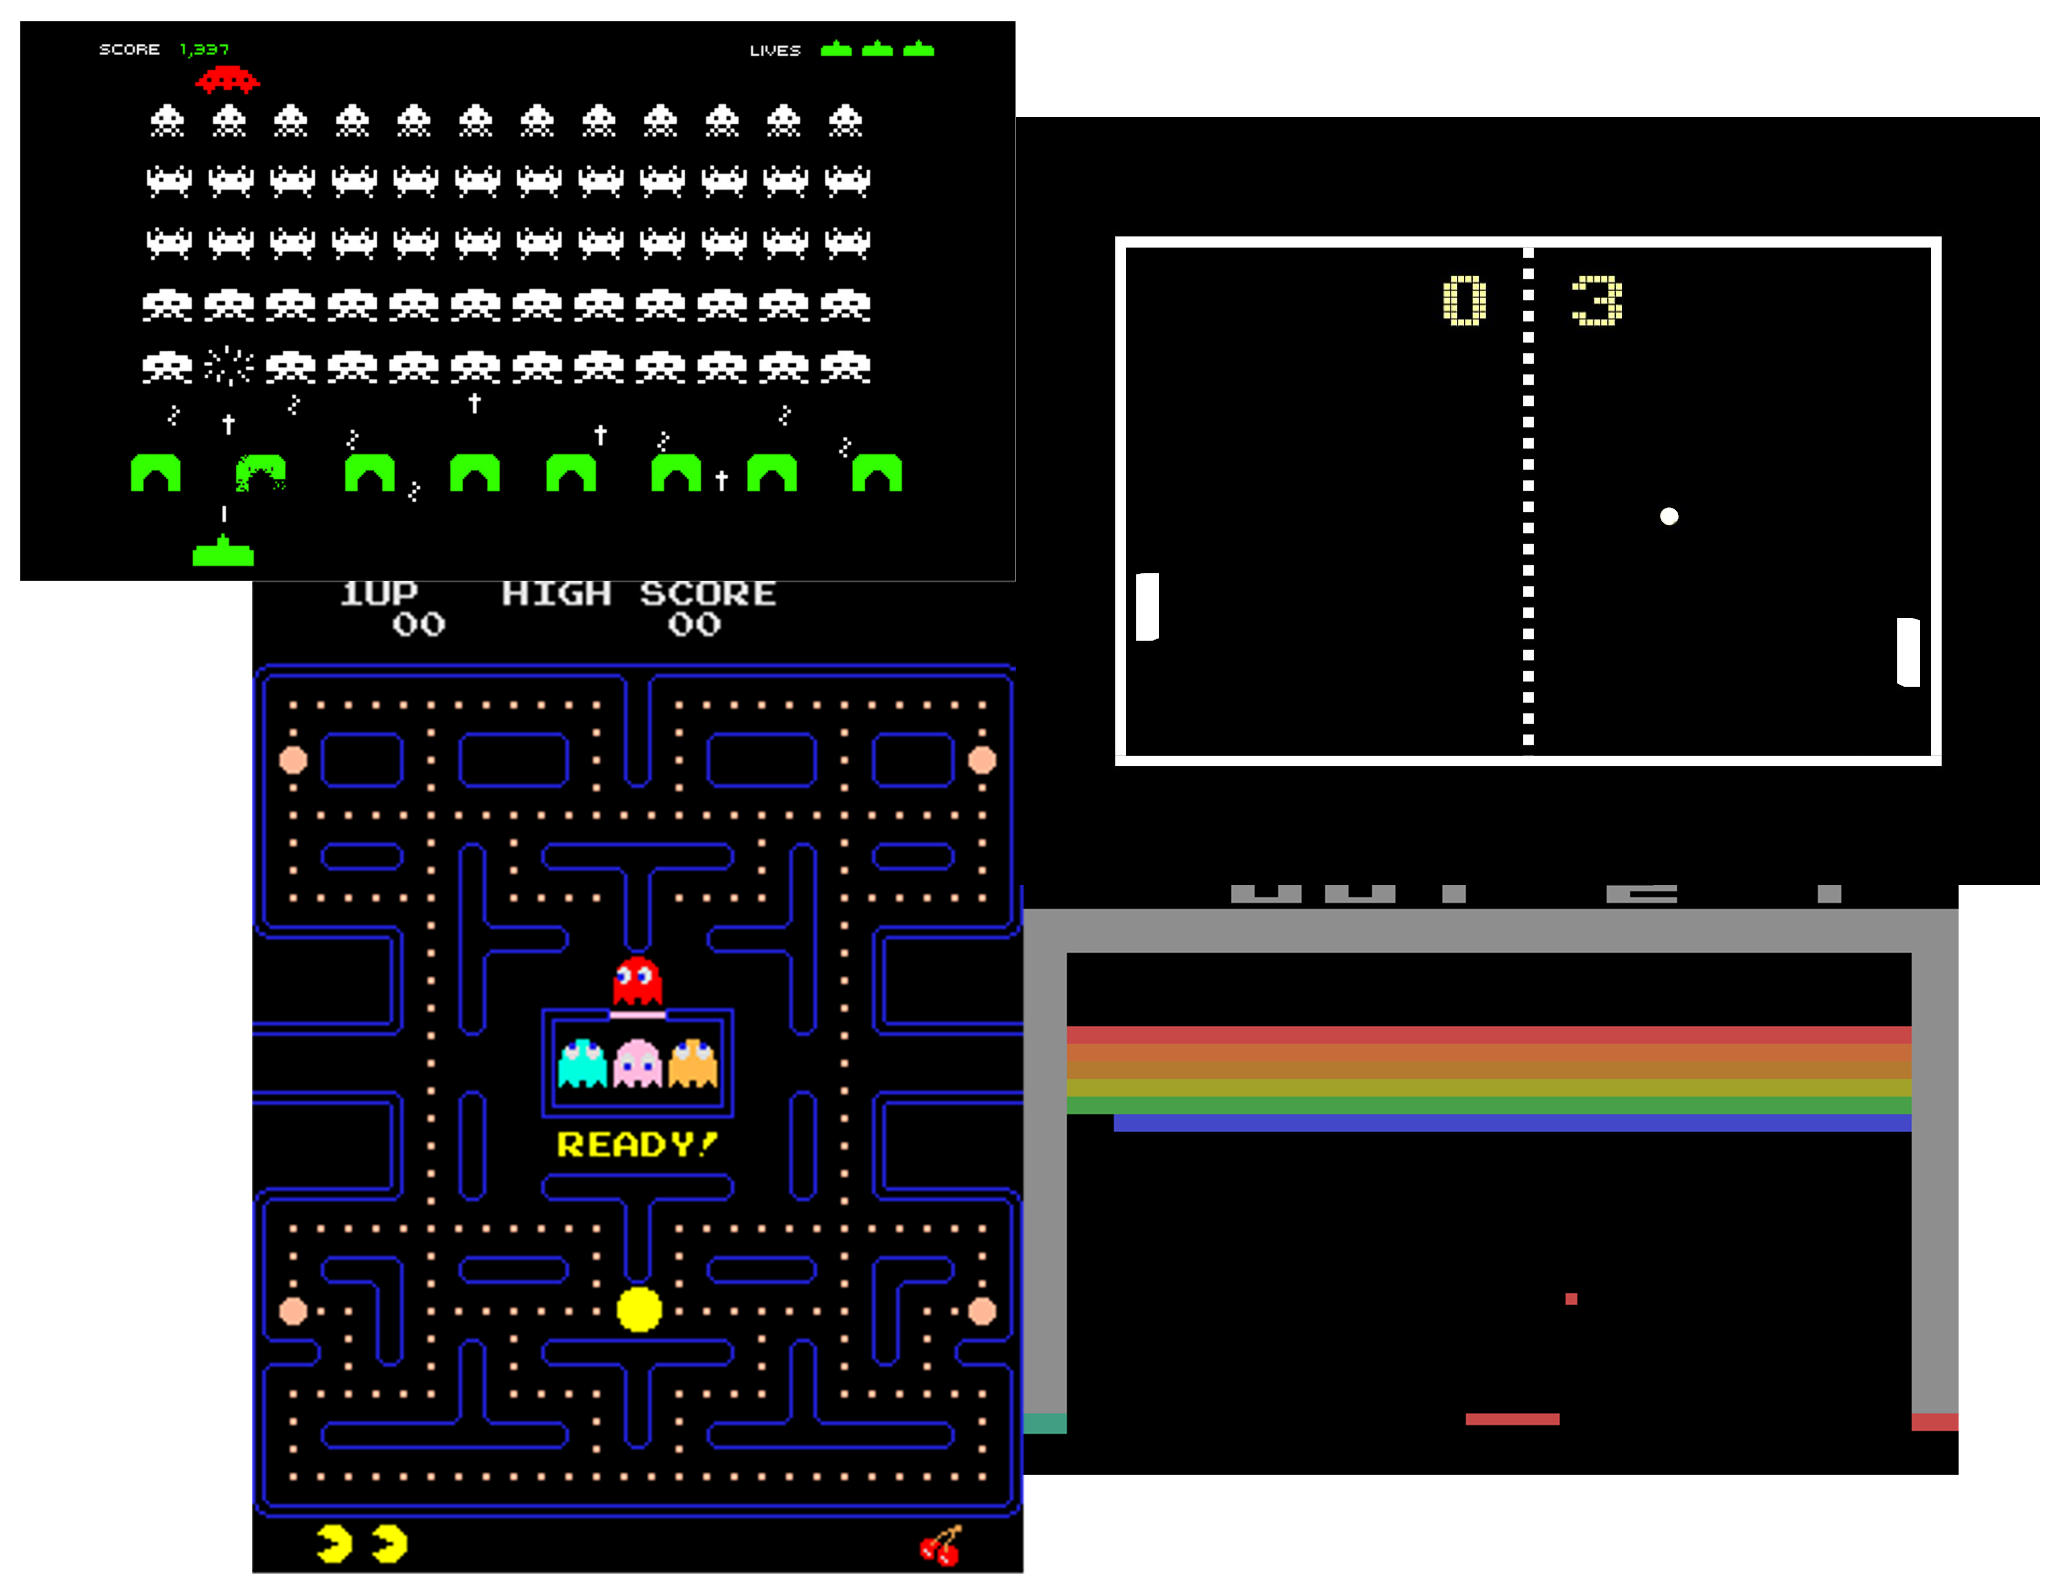
\includegraphics[width=\linewidth]{./images/Introduction/imagdle1970.png}
		\caption{Space Invaders, Pong,\\ Pacman et Breakout}
	\end{figure}	
\end{minipage}\hspace{.04\textwidth}\begin{minipage}[t]{.48\textwidth}
	\subsubsection{1980}
	\begin{figure}[H]
		\center
		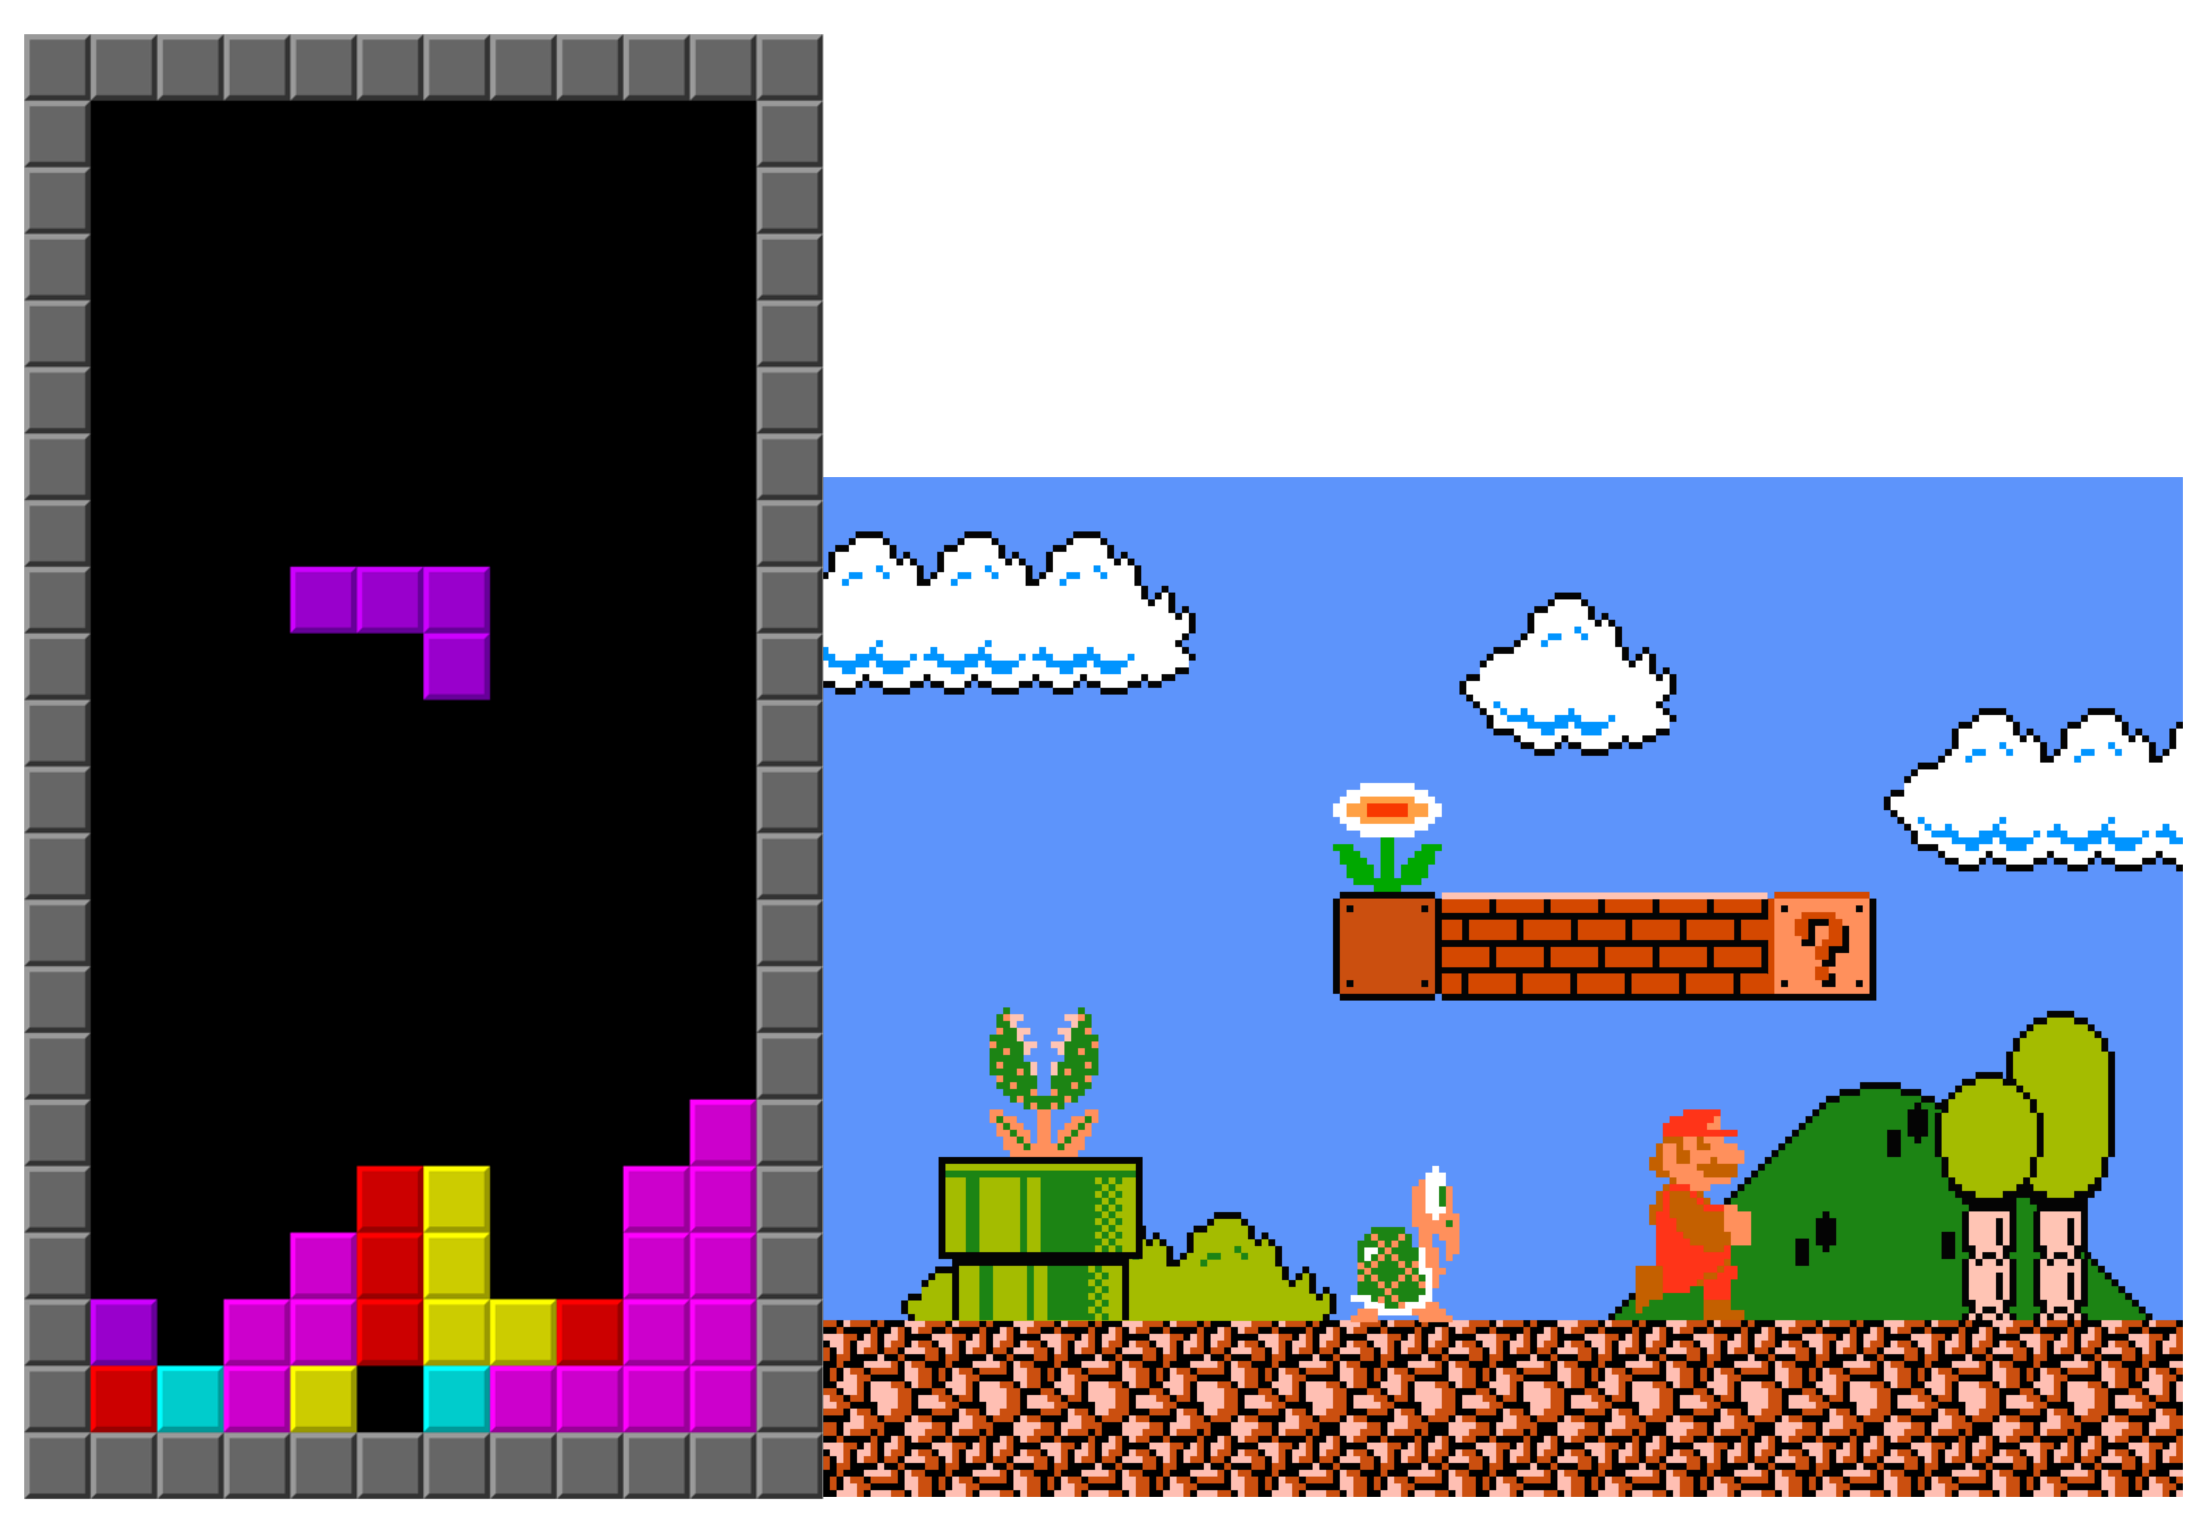
\includegraphics[width=\linewidth]{./images/Introduction/imagdle1980.png}
		\caption{Tetris et Super Mario Bros}
	\end{figure}
\end{minipage}

\begin{minipage}[t]{.48\textwidth}
	\subsubsection{1990}
	\begin{figure}[H]
		\captionsetup{format=myformat}
		\center
		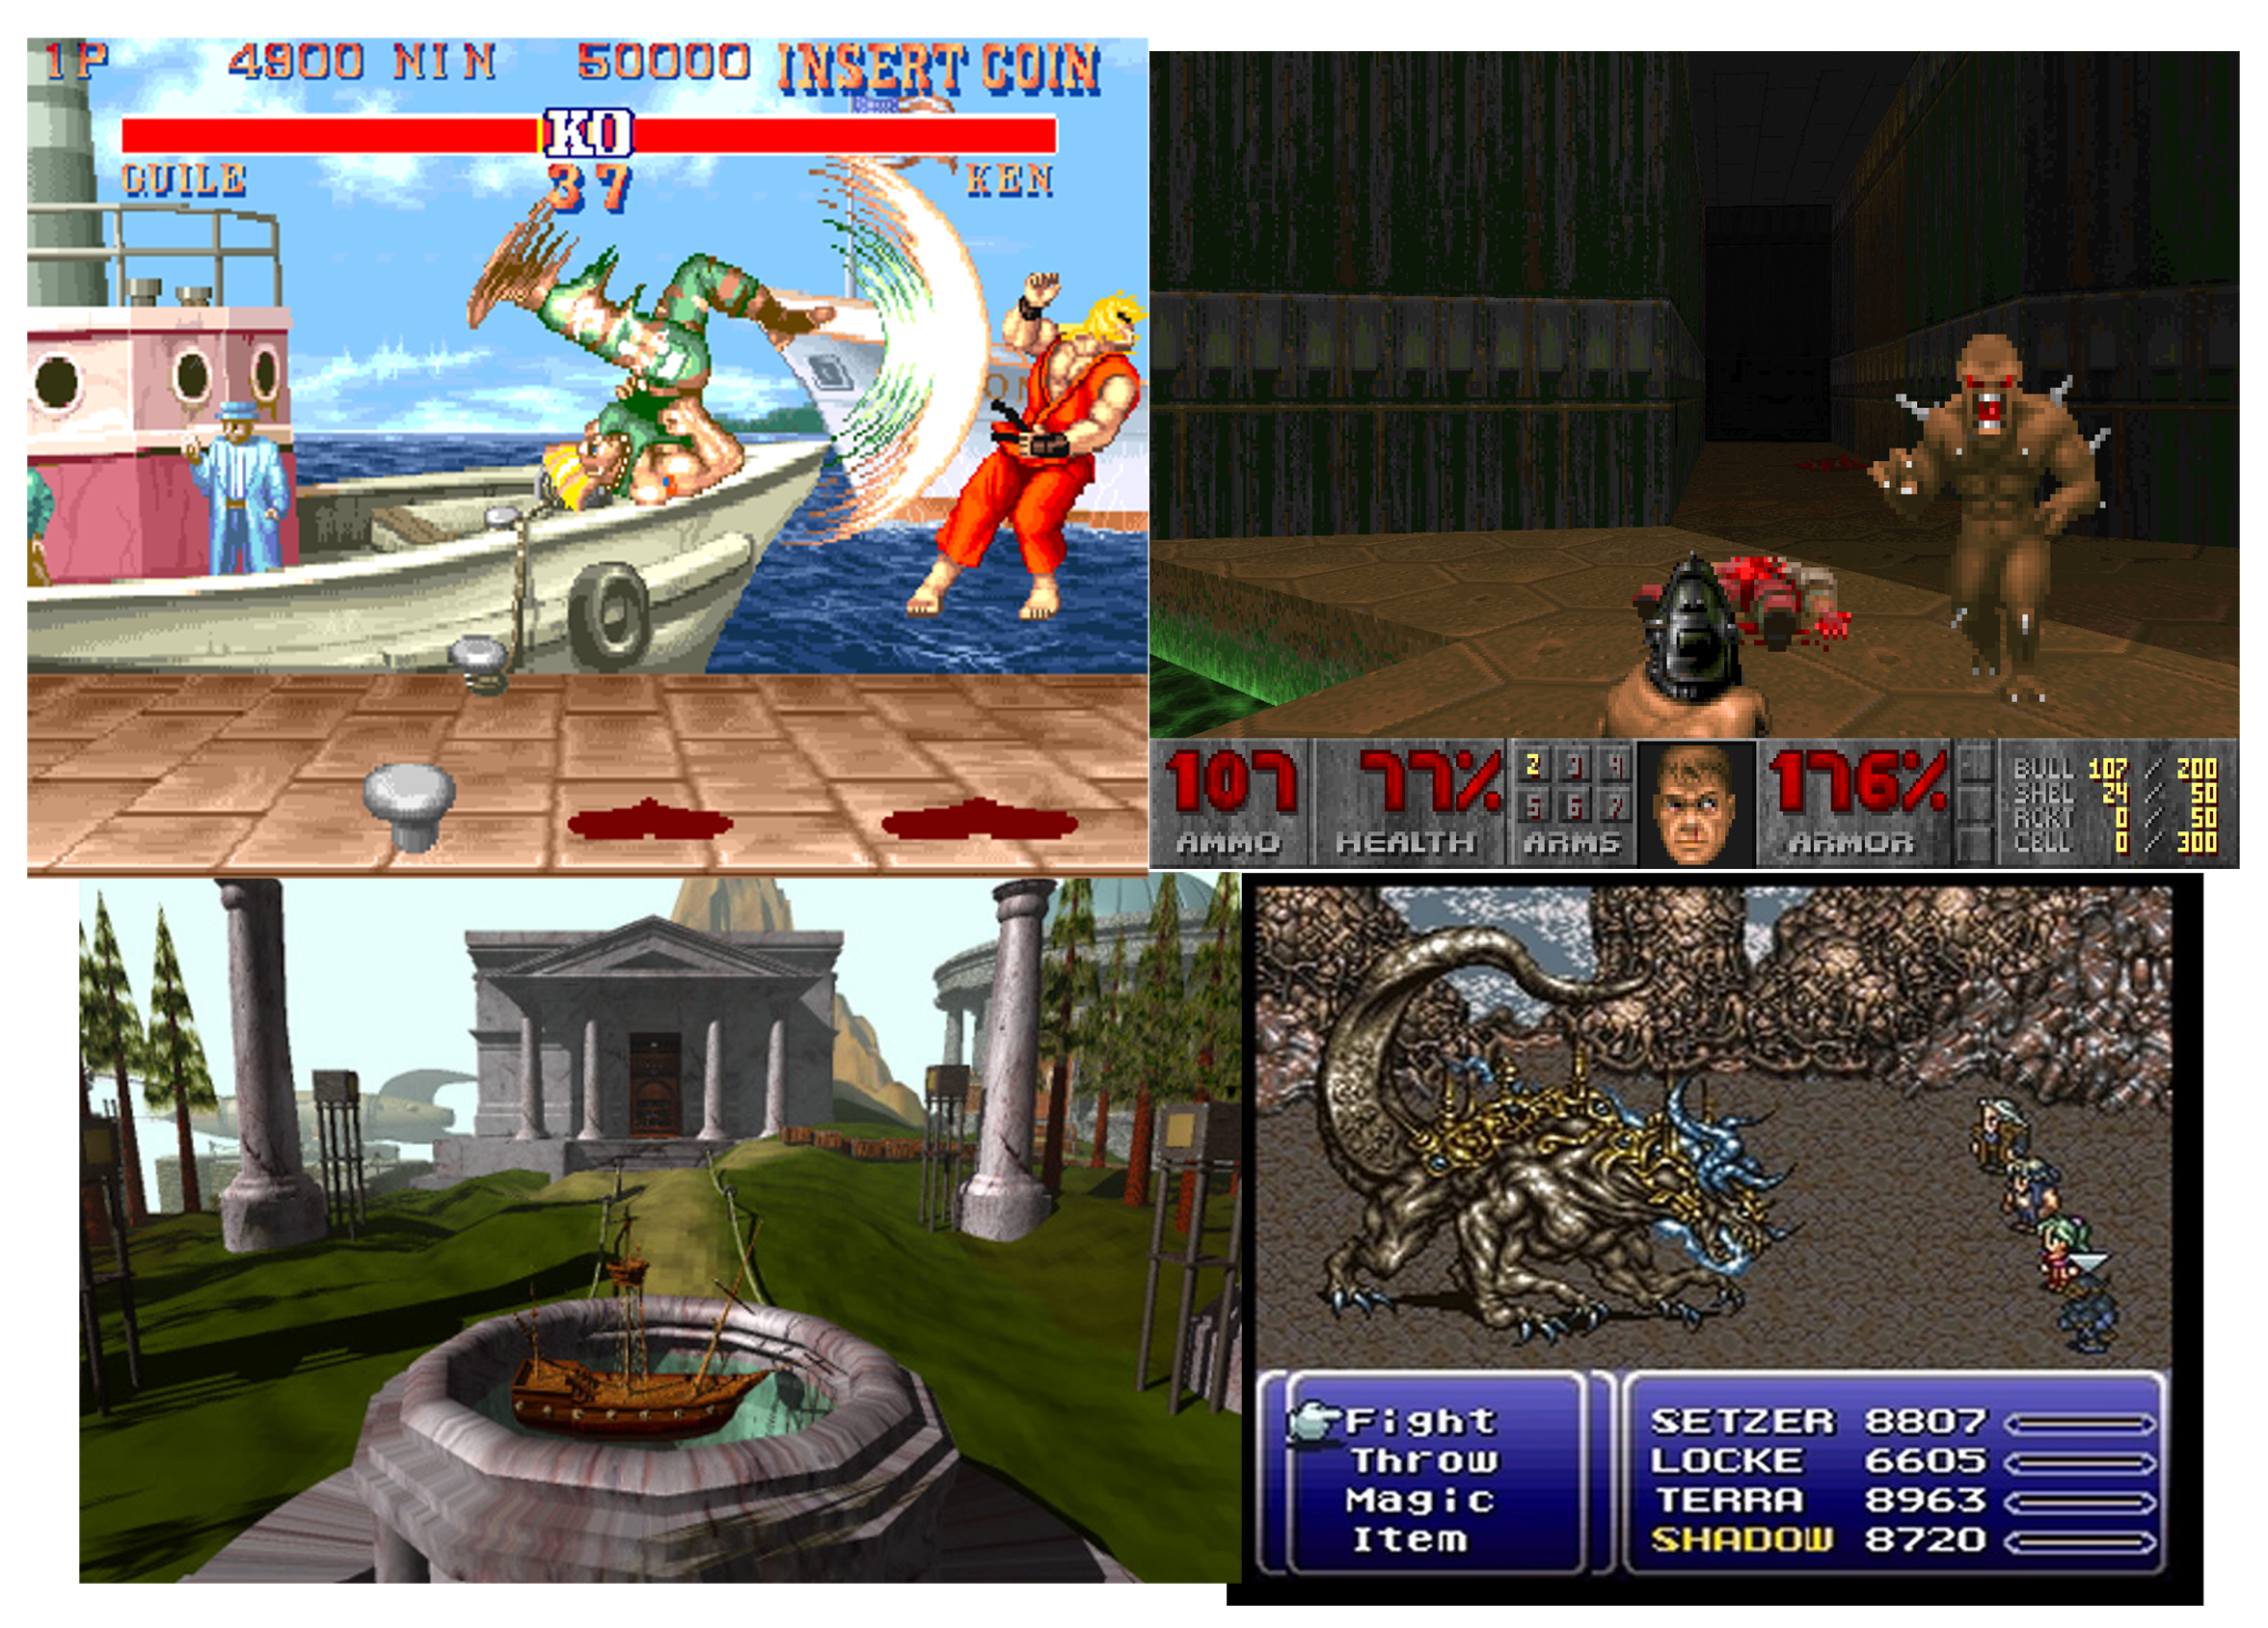
\includegraphics[width=\linewidth]{./images/Introduction/imagdle1990.png}
		\caption{Street Fighter II, Doom,\\ Myst et Final Fantasy VI}
	\end{figure}
\end{minipage}\hspace{.04\textwidth}\begin{minipage}[t]{.48\textwidth}
	\subsubsection{2000}
	\begin{figure}[H]
		\captionsetup{format=myformat}
		\center
		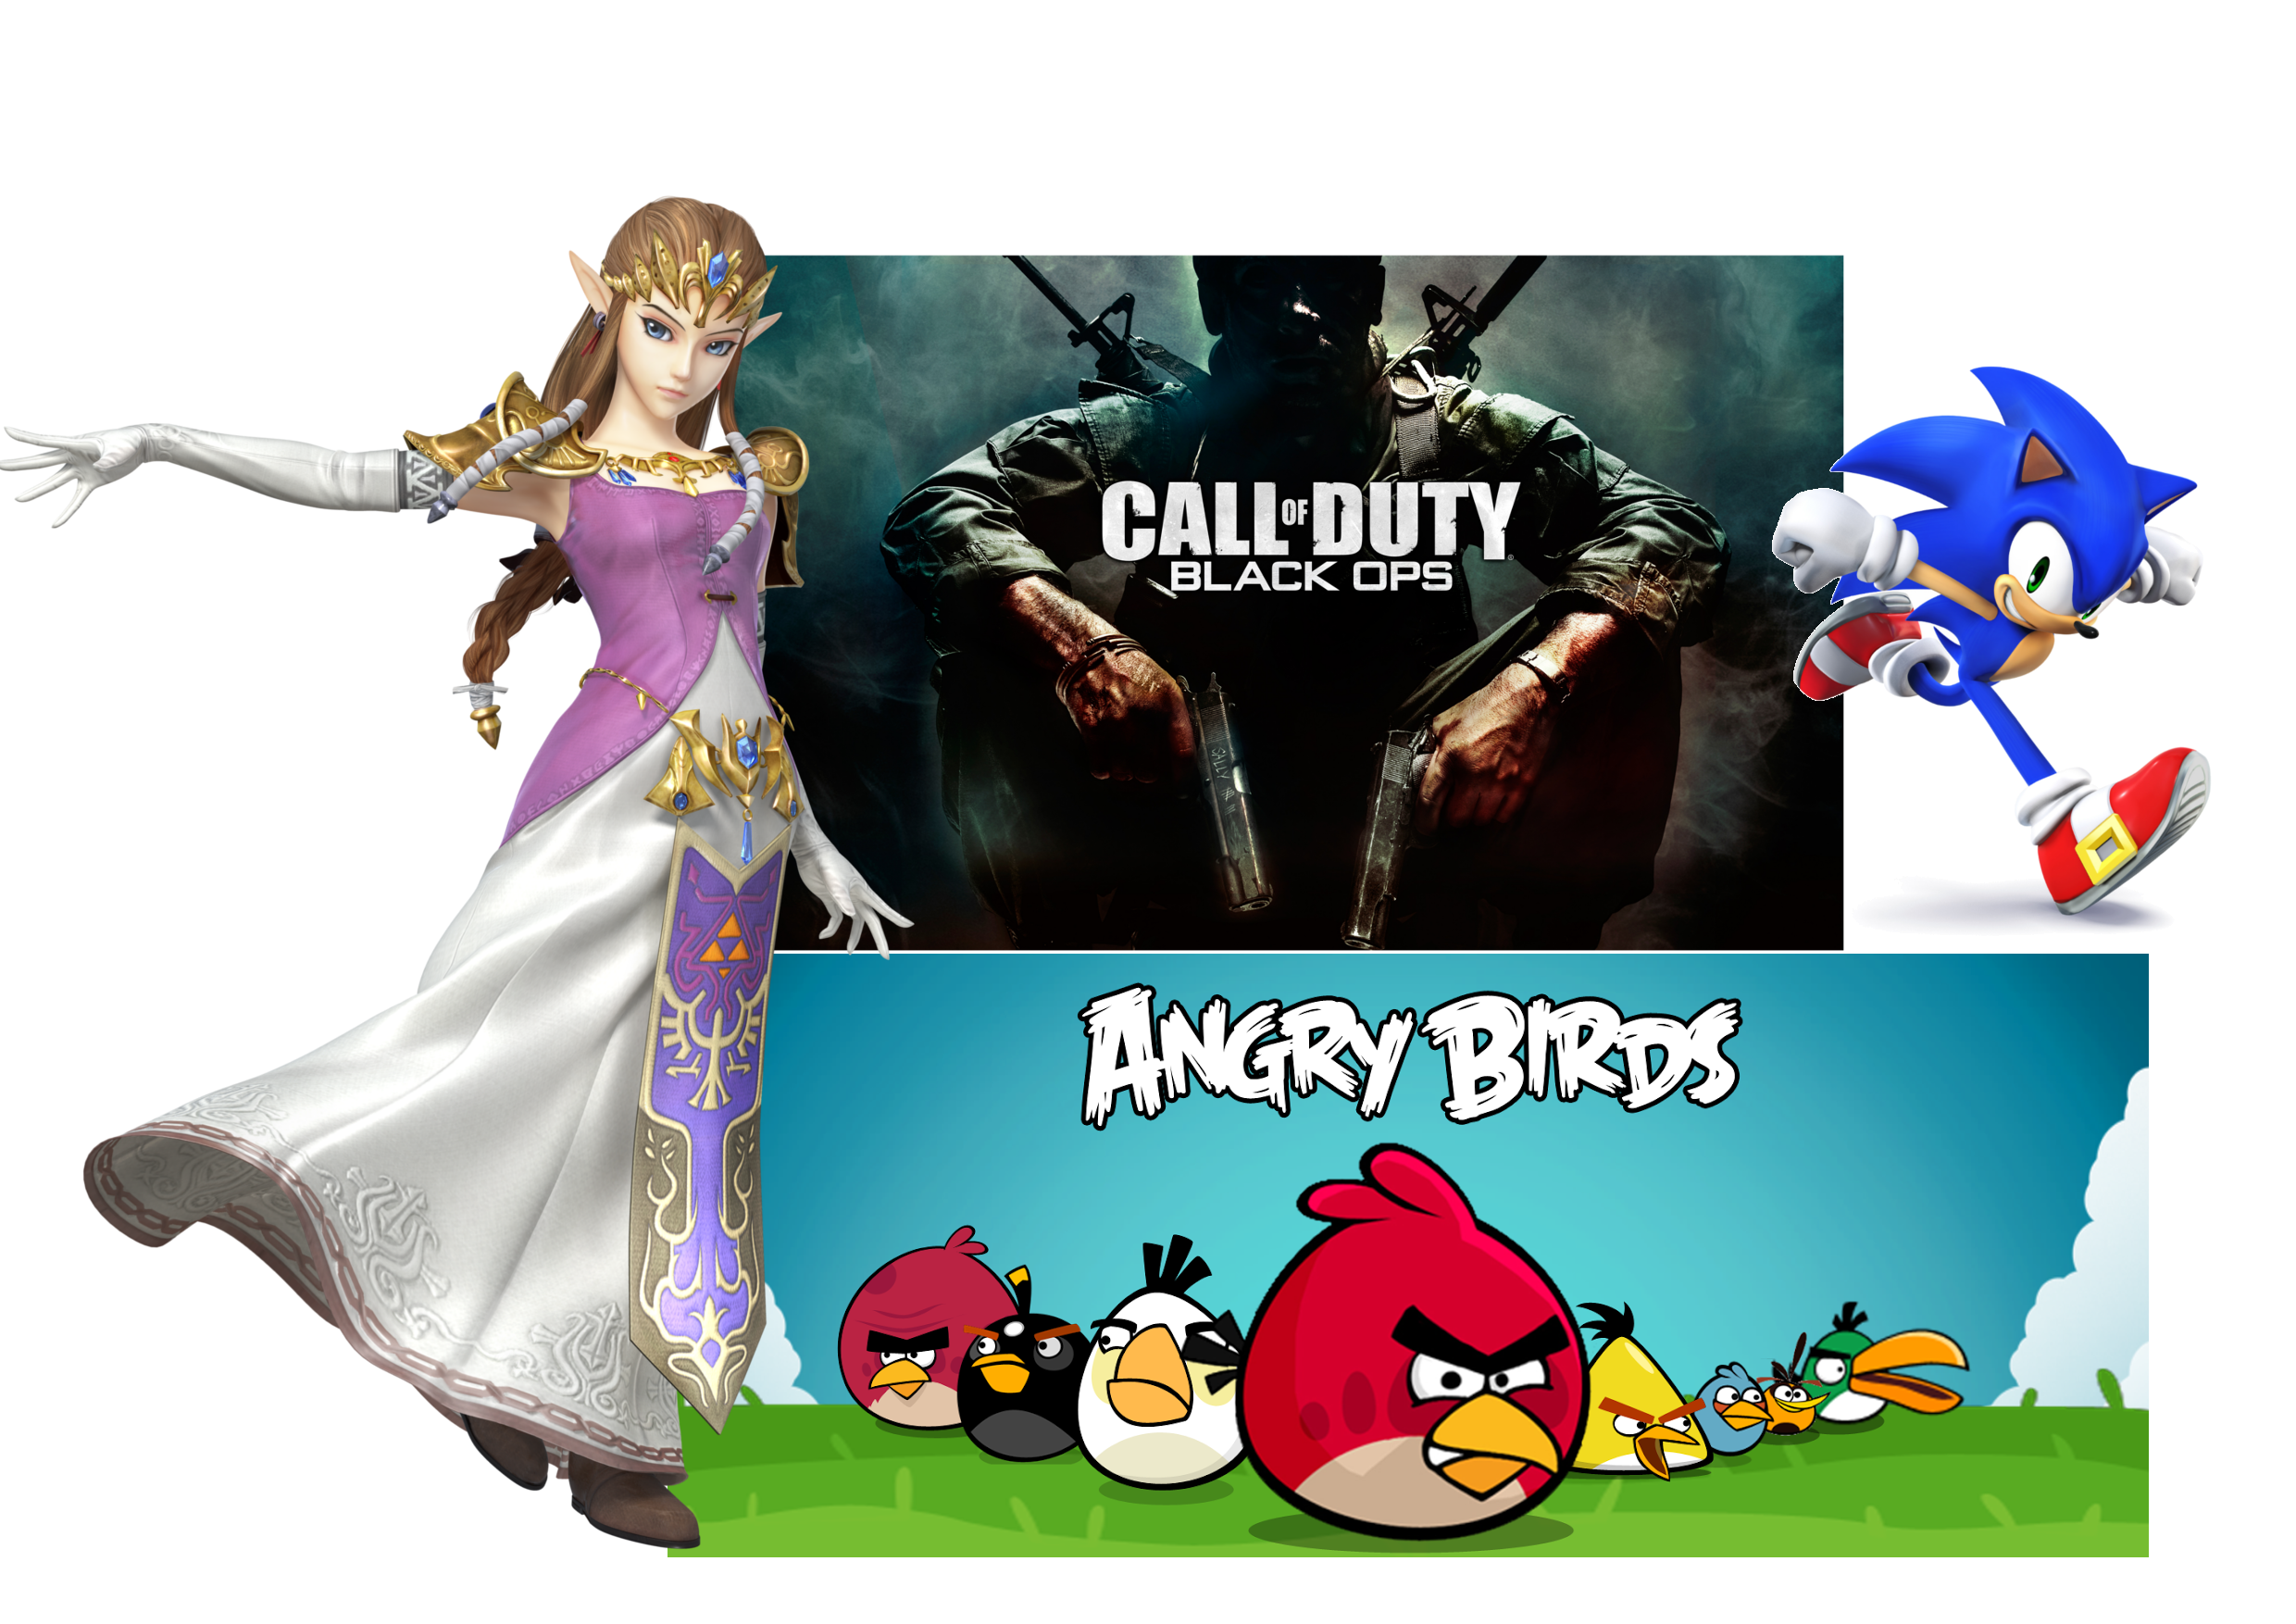
\includegraphics[width=\linewidth]{./images/Introduction/imagdle2000.png}
		\caption{Zelda, Call of Duty,\\Sonic et Angry Birds}
	\end{figure}
\end{minipage}
\vspace{\baselineskip}



\chapter{Création d'un univers}
\printMiniToc



\begin{note}
	Dans cette partie, j'expliquerai les détails de l'univers que j'ai créé pour ce jeu ainsi que les raisons qui m'ont poussé à faire les choix menant à cette fiction. L'univers n'est cependant pas terminé; s'il suffit largement aux besoins du jeu, il pourrait, dans l'optique de la réalisation d'une version complète, être agrandi et complété. De plus, certains détails, exprimés dans ce texte, dépassent déjà la portée de la démo.
\end{note}



\section*{Les thèmes importants pour le jeu}
Comme je l'ai déjà indiqué dans la section \ref{sec:objectifsTM}, ce jeu est l'occasion pour moi de développer des thématiques qui me semblent importantes. C'est un jeu d'opinion qui se veut le défenseur de mes points de vue.

Le thème le plus important est la relation humaine à la Nature. J'ai toujours été fasciné par la beauté de cette dernière, sa cruauté, à la fois son ordre parfait et son désordre total. Pour moi, un retour à la Nature est une condition nécessaire pour atteindre le bonheur. La relation que nous entretenons avec elle, collaborative ou dominante, sera donc au c\oe ur du jeu et ce choix déterminera de nombreux aspects de l'histoire et du gameplay\definition.

Il existe cependant de multiples contradictions entre ma passion pour la Nature et l'univers qui m'entoure. Comment ne pas constater les dégâts que nous infligeons à notre environnement? Mais plus encore, comment ne pas constater que notre mode de vie (que certains nomment consumérisme) a perdu toute sa simplicité, son sens, sa \enquote{naturalité}. Ce jeu sera donc l'occasion de mettre le doigt sur ces paradoxes et l'opportunité de se poser certaines questions sur nos façons de faire.

Un autre thème conducteur sera la relation fraternelle (sororale dans le cas du jeu); sujet important à mes yeux, étant donné que j'ai moi-même un frère. Le jeu gravitera aussi autour de la question de l'utilisation bénéfique et responsable ou destructrice et irresponsable de la technologie, des améliorations qu'elle peut apporter ou des dommages qu'elle peut causer et des abus auxquels elle peut conduire. Finalement, la question de la religion sera abordée, bien que dans une moindre mesure: quelle utilité a-t-elle? à quelles dérives peut-elle mener?


\section{Un monde divisé entre deux peuples}
Le jeu se déroule dans un univers, nommé \nomUnivers, qui est principalement divisé entre deux peuples: les Humains et les \nomNaturels s.

Les Humains sont une faction terne, grise et soumise à un tyran: Lord Gaamon. Le despote, atteint de folie, a une peur viscérale de la Nature et a convaincu le reste de la population de sa nocivité. L'utilisation de technologies mécaniques, polluantes et parfois brutales est monnaie courante et permet aux hommes de dominer les autres peuples habitant \nomUnivers; mais cela ne peut se faire sans ravager l'environnement. Ce peuple perdu et sombrant dans la peur a, pour sa plus grande majorité, oublié son histoire et exécute les ordres de Gaamon sans sourciller. Mais si certains hommes se laissent aller à la violence ou l'obéissance, d'autres à l'inverse tentent de résister physiquement, ou mentalement du moins. Ce sont les \enquote{Naturels}, mais ils ne représentent qu'une petite minorité de la population totale. La population humaine vit enfermée dans \nomVille, une ville énorme, entourée de hautes murailles. Les Humains représentent un peuple perverti, apeuré et aveugle.

Les \nomNaturels s, à l'inverse des Hommes, représentent un peuple plus pacifique qui accorde beaucoup d'importance à la Nature et tente de vivre en accord avec elle. Le nom \enquote{\nomNaturels s} est une anagramme de \enquote{Naturels} et pourrait se rapporter à l'adjectif \enquote{tellurique} qui signifie \enquote{de la terre}. Ce peuple est cependant sur le déclin. Autrefois au sommet de son art, c'est maintenant une nation dont les fondations même s'effritent.


\section{Les Humains}

\subsection{L'histoire humaine en quelques mots}

\begin{note}
	Cette section décrit en quelques mots l'histoire des hommes. Certains détails supplémentaires sont décrits à la section \ref{sec:HistoireGaamon}.
\end{note}


20 ans avant le début du jeu, la ville n'était encore qu'un petit village agréable, nommé Murtos. La vie agricole, bien que rude et laborieuse, y était appréciée et rares étaient les histoires qui venaient troubler la quiétude des habitants. Mais tout cela changea le jour où le jeune Gaamon arriva...

L'étranger décida de s'installer dans le bourg et fonda, ce qui était alors une nouveauté, la première usine d'\nomUnivers. Son succès fut rapide: il apportait du travail et produisait beaucoup grâce aux machines qu'il construisait. Il agrandit bientôt son usine... puis en construisit une deuxième, qu'il agrandit aussi. Grâce à cela, les conditions de vie s'améliorèrent, tout le monde avait du travail et la population était heureuse de cette venue providentielle.

L'ambition de Gaamon étant véritablement grande, il fit construire d'autres usines, créa d'autres machines, employa bientôt tout le village et draina les populations des alentours dans ses halles de production. Les affaires allaient bon train, l'argent coulait à flots et son influence ne cessait de s'étendre.

\begin{wrapfigure}[11]{r}{.38\textwidth}
	\vspace*{-.8cm}
	\center
	\includegraphics[width=\linewidth]{images/Monde/drapeauGaamonLarge.png}
	\caption{Emblème de Gaamon}
\end{wrapfigure}

Avec les années, il fédéra tous les Humains sous la bannière unique de ses usines et devint le maître incontesté de ce qui était devenu une ville. Mais Gaamon n'était pas complètement sain d'esprit; cachée au fond de lui résidait une folie haineuse de la Nature. Le pouvoir et l'argent permirent à cette phobie, jusqu'alors refoulée, de s'exprimer de plus en plus pleinement et ouvertement. Il avait réussi à industrialiser, mécaniser le village, il voulait maintenant étendre son emprise hors des limites de la cité.

Il fortifia la ville en construisant des murailles et bâtit, en son centre, une immense tour d'acier et de verre qui devint l'icône emblématique de son empire. Il imposa à tous l'interdiction de sortir de l'enceinte des murs et brûla les dernières traces de verdure dans la cité. Il s'engagea alors, depuis le haut de sa nouvelle forteresse, dans un projet d'éradication plus vaste, qui annihilerait toute Nature, plantes ou animaux, des terres environnantes. Le jeu débute quelques années après le commencement de ce funeste projet, à l'intérieur de la ville.

\vspace*{-1mm}
\subsection{Petite biographie de Gaamon}
\begin{figure}[p]
	\center
	\thisfloatpagestyle{empty}
	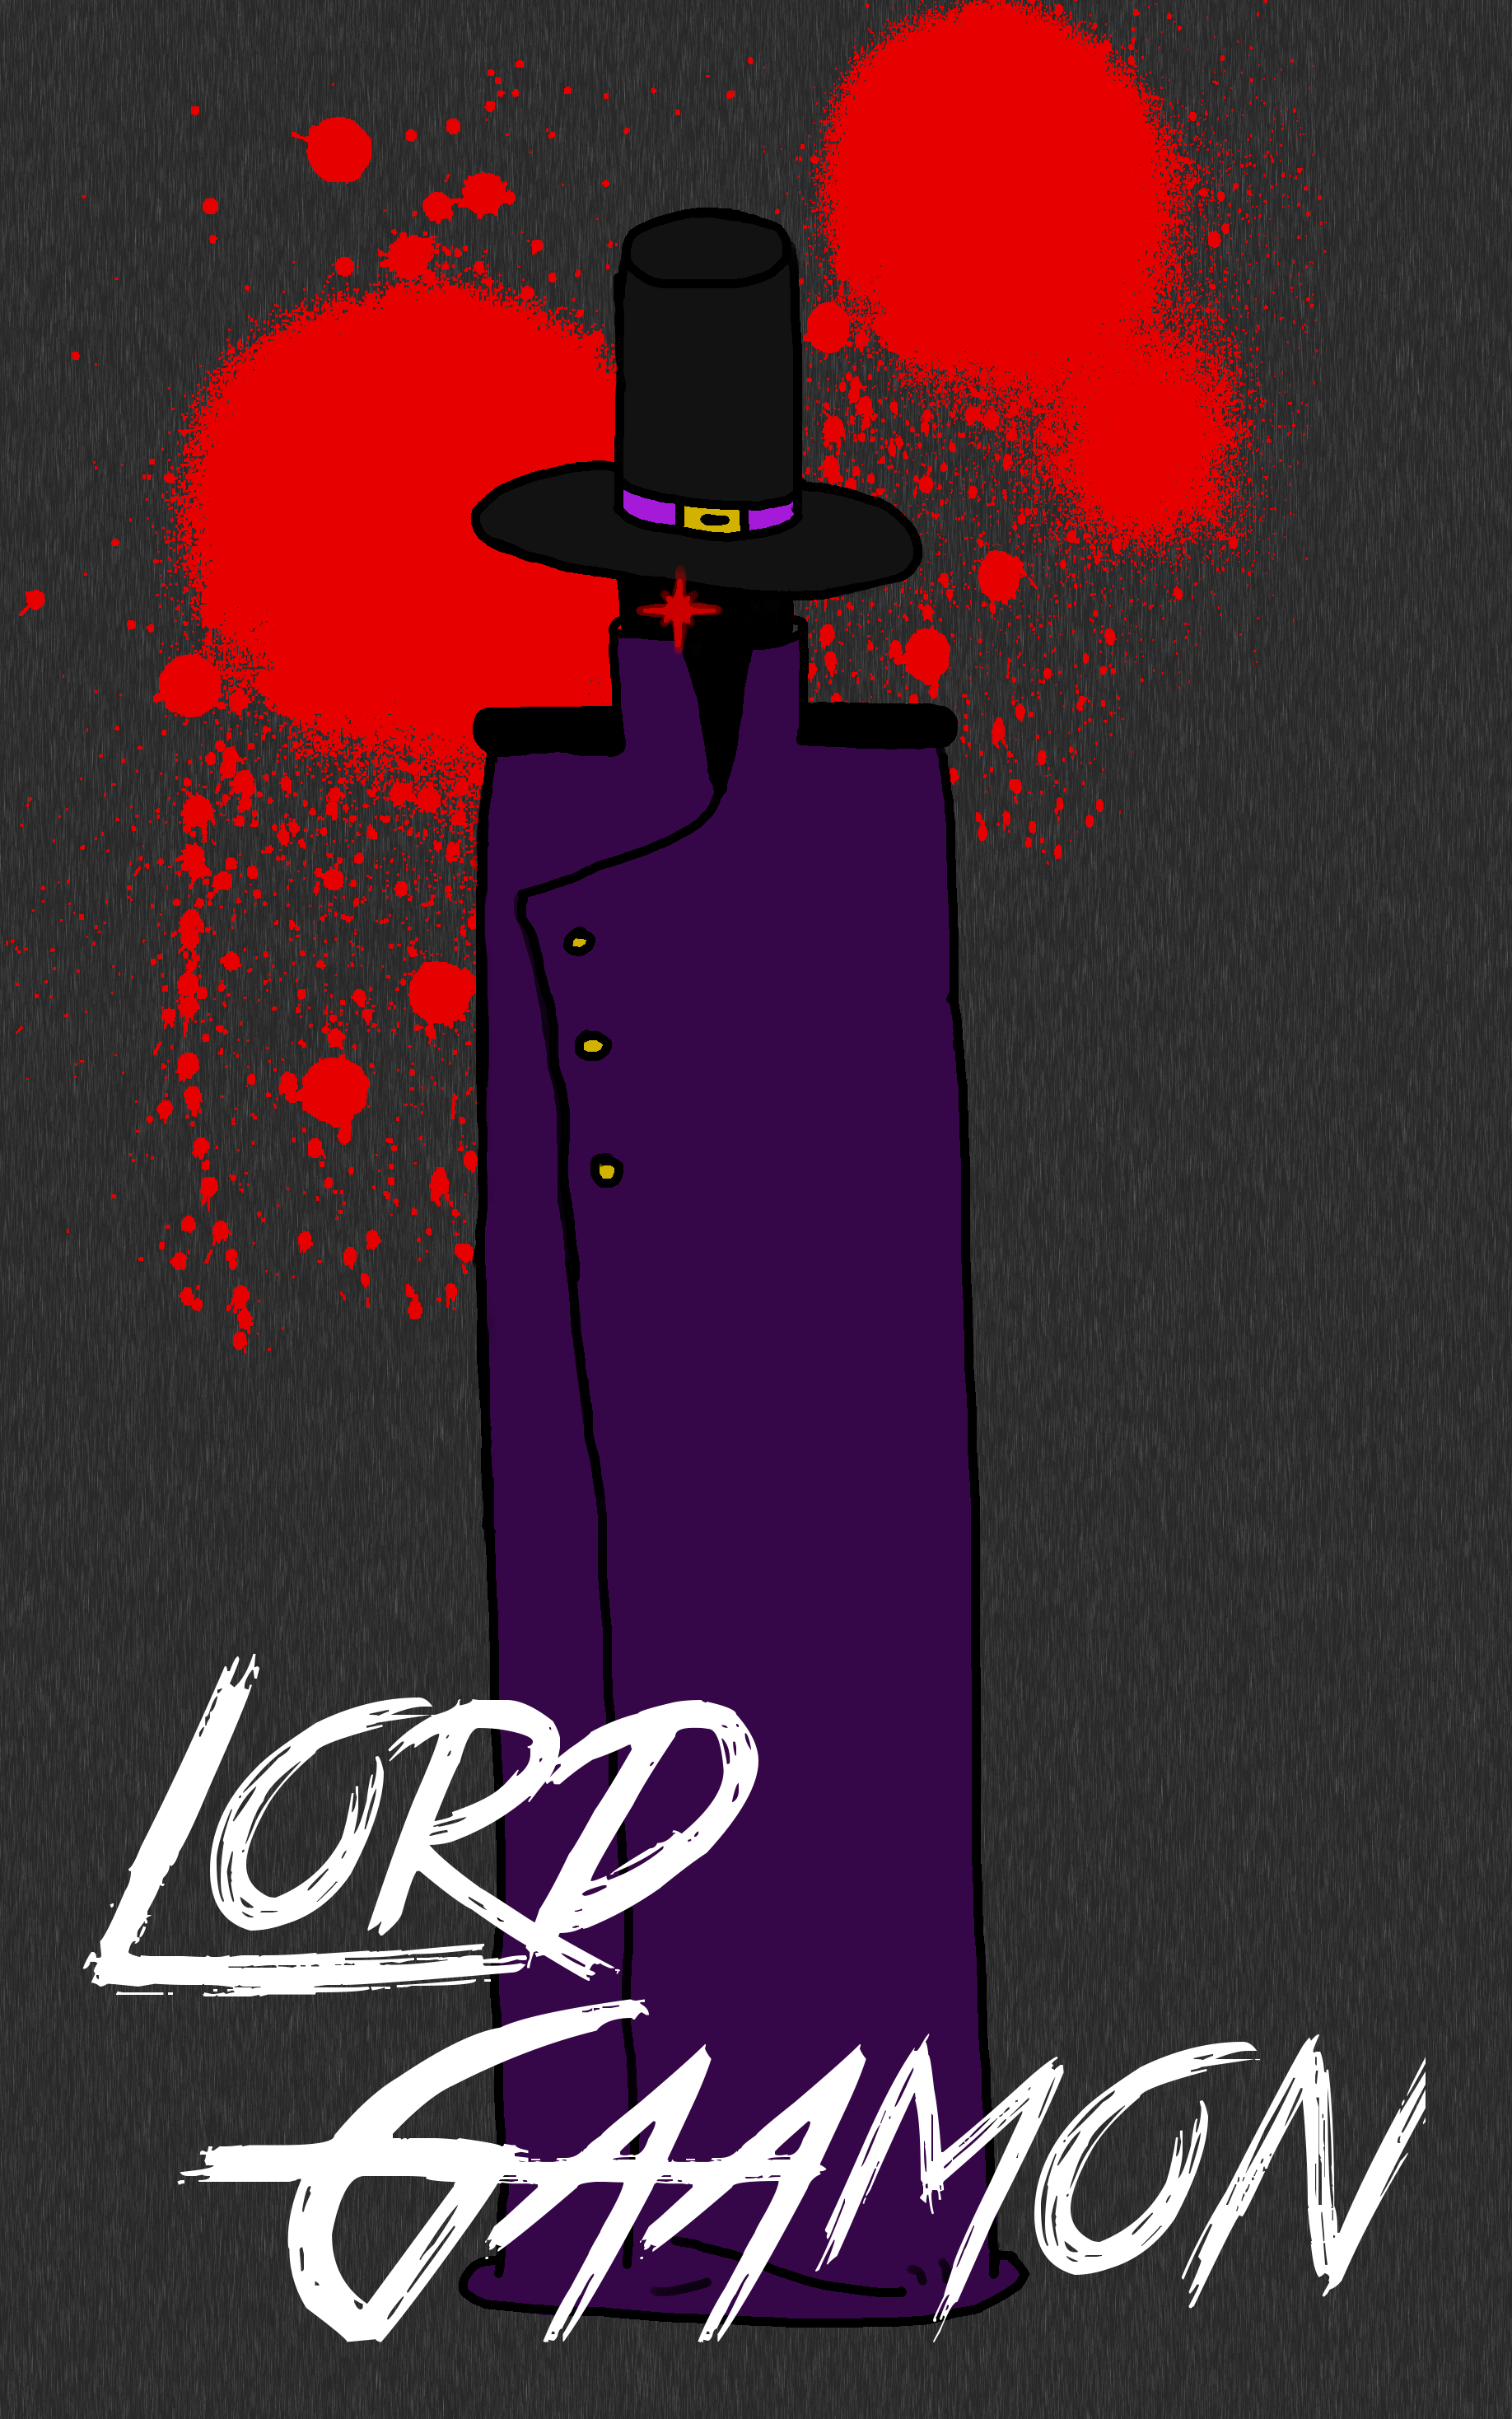
\includegraphics[width=\textwidth]{./images/Monde/Personnages/gaamonPortrait.png}
	\caption{Lord Gaamon\label{fig:Gaamon}}
\end{figure}

\vspace*{-2mm}
\descrPersoTitle[0]{Ses habits}
Gaamon est vétu d'une longue cape violette et d'un haut de forme masquant son visage par l'ombre qu'il créer. Il est aussi muni d'un \oe il mécanique rouge luisant (\textit{cf.} figure \ref{fig:Gaamon}).

\descrPersoTitle{Ses caractéristiques principales}
Il dirige la ville d'une main de fer depuis le haut de sa tour, il déteste la Nature au plus haut point et veut l'éradiquer par tous les moyens. Gaamon est doté d'une capacité innée à jouer avec les engrenages et les pistons; il a toujours eu un don pour la création de machines. Il en imaginera quantité; au départ pour aider dans ses usines, puis d'autres plus compliquées comme les Gnobols (\textit{cf.} section \ref{sec:Gnobols}) pour asseoir son empire.

\newpage
\descrPersoTitle{Son histoire}
\label{sec:HistoireGaamon}
\textbf{Adolescent}\quad Gaamon était un jeune homme plein de vie, d'enthousiasme et de bonne humeur. Son charisme indéniable semblait le promettre à un avenir radieux et, aimé de tous --- villageois comme camarades de jeu, il profitait innocemment de ce temps joyeux.

Mais lors de ce jour maintenant mille fois maudit par les dernières populations libres d'Éluria, il se perdit en forêt suite à un jeu avec ses amis. Il pénétra profondément dans ce lieu mystérieux avant de se rendre compte qu'il ne savait plus d'où il venait ni comment sortir. Seul et désemparé, il cria à l'aide, en vain, chercha, cria de nouveau, se mit à courir, mais la forêt se refermait sur lui, les branches lui griffaient le visage et les racines cherchaient à le faire trébucher. Il tenta de trouver la lisière et, ce faisant, ne s'enfonça que plus profondément dans cet univers à la fois plein d'enchantements et de maléfices. Son errance dura tant et si bien, qu'il finit par atteindre le c\oe ur même de la forêt, un lieu hautement sacré, réservé aux seuls esprits et rares élus, un lieu protégé par de multiples pièges et sortilèges afin d'en écarter les intrus.

Un de ces pièges se referma sur lui: il marcha sur un champignon empoisonné qui libéra brutalement ses spores vaporeux. Ces puissants psychotropes plongèrent le jeune homme dans un état de démence hallucinatoire très profonde. Il perdit toute conscience de la réalité et vécut l'horreur et la peur sous toutes leurs formes les plus profondes durant des heures, seul au c\oe ur de cet écrin terrifiant.

Personne ne sait comment, mais le garçon sortit de la forêt deux jours plus tard, ses vêtements en lambeaux, l'âme déchirée. Il lui fallut un peu plus de deux ans pour recouvrer la raison, mais jamais plus il ne fut le même. La vie perdit à ses yeux toute magie, devint terne et cruelle. Mais surtout, il emporta dès lors avec lui une peur absolue et une haine encore plus profonde de la Nature. Il restait un jeune homme beau, intelligent et malin mais il avait perdu l'espoir, la joie de vivre.

\textbf{Jeune adulte}\quad Quelques années plus tard, alors que le commerce de Gaamon à Murtos commençait à s'épanouir, il rencontra Miya; une jeune femme à la beauté exquise, particulièrement vive d'esprit, singulièrement perspicace et follement amoureuse de la vie, de sa simplicité et de sa beauté. Gaamon, immédiatement intrigué, voulu connaître cette personne si différente de lui et en même temps tellement séduisante. L'attraction fut réciproque et Miya fascinée, tant par la beauté ténébreuse que par l'esprit torturé mais néanmoins redoutable du jeune homme, fut pour ce dernier une lumière dans sa vie alors si sombre. Serait-elle celle qui lui permettrait de retrouver la joie de vivre?

Ils débutèrent une relation à la fois passionnée, fusionnelle et charnelle, vivant un bonheur profond et léger. Miya eut son premier enfant --- une magnifique fille --- au solstice d'été. Ils la nommèrent Lenaï comme l'héroïne d'un conte enfantin qu'ils affectionnaient tous les deux\footnote{Pour approfondir encore l'univers d'\nomUnivers, il pourrait être intéressant d'écrire un conte narrant l'histoire des Hommes et des Telurans au commencement de ce monde. Il pourrait avoir une signification particulière pour Gaamon et lui rendre un peu sa joie de vivre et son humanité quand il l'entend. Il pourrait être inséré dans le jeu comme une cinématique en images fixes (\textit{cf.} section \ref{sec:quatriemeActe} à ce sujet).}.

Le lien qui unissait les deux âmes éprises était très fort, particulièrement heureux et semblait augurer d'un avenir des plus brillants. Cependant, si Miya permettait au garçon de retrouver la joie de vivre, elle n'avait pas la capacité d'annuler sa haine pour la Nature. Et, les affaires de Gaamon, marchant bien, trop peut-être, lui permettaient d'assouvir ses volontés vengeresses. Il commença modestement et fit remplacer un parc par un immeuble, puis installa à l'emplacement de l'étang à la périphérie du village un centre d'épuration qui raya ce dernier de la carte. Ce fut ensuite au tour de la forêt avoisinante d'être rasée et remplacée par des usines. Au fil des mois, plus son influence grandissait, plus ses intentions devenaient évidentes.

Il fonda un parti --- le parti industrialiste --- qui rallia la majorité de la population, constatant bien que Gaamon apportait un confort de vie tout à fait révolutionnaire. Il cherchait principalement à rationaliser et améliorer les flux de production pour augmenter le bonheur général, mais ces idées étaient pour lui indissociables d'une haine destructrice contre la Nature. Un parti opposé vit le jour quasi simultanément, fondamentalement opposé aux idées du premier. Il prônait une idée de Nature et de paix, de simplicité et de bonheur. La guerre entre les deux fut immédiate. Toute proposition de l'un était immédiatement saluée par une contre-proposition de l'autre, contre chaque projet étaient déposées des motions, à chaque discours on constatait la présence d'opposants remontés.

Gaamon faisait tout son possible pour mettre des bâtons dans les roues de son adversaire politique, saper sa crédibilité et lier toujours plus de personnes à sa cause. À terme, sa stratégie eut les effets escomptés. Il réussit à discréditer les naturels et la plupart des habitants prirent fait et cause pour lui. Il leur avait apporté, à lui seul, confort, aisance et longévité.

Si le combat, au départ, était équilibré, la balance penchait soudain très fortement de son côté. Il se fit élire maire du village qui prenait de plus en plus l'apparence d'une ville et entreprit tout ce qu'il fallait pour réduire à néant le parti naturel. Interdiction de manifester, utilisation d'espions et d'agents doubles pour semer le trouble dans les rangs adverses, raids nocturnes pour apeurer les membres; toutes les stratégies étaient bonnes. L'interdiction totale du parti, finit de dissoudre l'entité politique et seul un groupuscule clandestin subsista.

Miya n'avait jamais senti le besoin de s'inscrire dans quelque combat politique que ce soit et se contentait de vivre heureuse dans le monde protégé et douillet qu'elle avait créé autour de son enfant. Elle profitait du temps qu'elle avait et suivait de loin les disputes incessantes sans pour autant y prendre part. Si elle devait appartenir à l'une des factions, ce serait celle des naturels; mais pourquoi faire? Quel intérêt y avait-il à prendre part à ce conflit, si ce n'était l'alimenter plus encore?

Petit à petit Gaamon pris le contrôle de la ville. Les conditions de vie changeaient, les murs des bâtiments s'élevaient toujours plus haut comme ceux d'une prison, les frontières avec la Nature étaient sans cesse repoussées et le tapis urbain semblait vouloir s'étendre sans fin pour former un entrelacs infini de routes et de bâtiments.

\textbf{Quelques années à peine plus tard}\quad Ces modifications amenèrent des tensions dans le couple; les disputes, jusque-là inexistantes, devinrent plus courantes. Miya ne pouvait comprendre la haine de son mari pour ce qu'elle considérait être une source vitale pour chaque homme. Elle ne pouvait cautionner la dynamique qu'il tentait d'instaurer. Elle ne pouvait supporter la façon dont les naturels avaient été réduits au silence. Mais c'est peut-être le contact sacré avec la Nature, maintenant réduit à néant, cette absence qu'elle n'avait jusque-là jamais vécue, qui lui lacérait le plus le c\oe ur; pourrait-elle vraiment élever sa fille, Lenaï, sans jamais lui montrer les arbres naissants au printemps, les fleurs chatoyantes d'été, la douce mélodie des oiseaux à la saison des amours ou le chant du ruisseau pur? Tout cela paraissait impossible. Alors Miya, horriblement partagée entre son amour et sa passion pour la Nature, prit une décision impossible; elle allait entrer dans les factions de la résistance naturelle.

Ce revirement, la jeune femme l'assuma pleinement et décida d'en faire un combat personnel. Elle s'attela à combattre les projets anti-naturels de Gaamon avec vigueur. Rapidement, l'acharnement, la rage et l'audace de Miya, portèrent la jeune femme au rang de légende dans le groupe secret. Elle prit la direction des rebelles et appliqua les principes mêmes de Gaamon: organisation, rationalisation, répartition. Elle affûta leur stratégie et aiguisa leur volonté, afin d'avoir une véritable armée sous ses ordres; et engagea une guerre de l'ombre terrible et destructrice contre le tyran, contre cette personnalisation de la haine de la Nature, contre son plus grand et seul amour.

Miya entretint dès lors une double-vie: elle était simultanément la femme ayant choisi de suivre amoureusement son mari et une furie s'acharnant contre tout ce qu'il entreprenait, la mère chérissant sa fille et la cheffe la plus virulente qu'aient pu avoir les guerriers naturels, l'ennemi juré sabotant les plans et l'être aimé attendant patiemment au lit le retour de sa moitié. Cette situation dichotomique torturait son âme atrocement. De jour, elle aimait Gaamon, son esprit puissant et sa volonté à toute épreuve, son aura mystérieuse et sa force. Parfois, la jeune mariée se surprenait même à penser que l'homme en face d'elle voulait le bien de la population et améliorait vraiment le niveau de vie. Mais de nuit, elle redevenait l'esprit acéré, tranchant qui trouvait la gloire parmi les rangs de l'ombre. Elle utilisait toutes les informations glanées durant la journée pour empêcher la volonté industrielle de s'accomplir. Elle était l'agent double le plus redoutable, le plus insoupçonnable et le plus déchiré. Ainsi, le couple dirigeant était aussi le couple divisant.

Gaamon, aveuglé par la révolte et la ténacité dont faisaient preuve les rebelles, bâtit à la gloire de sa puissance les murailles qui entourent encore aujourd'hui la ville afin de la \enquote{protéger de la Nature extérieure}. Les immenses portes blindées à l'est et à l'ouest de la ville, seuls points de passage, n'étaient encore fermées que la nuit.

C'est à ce moment que Miya commença à avoir des doutes quant au but qu'elle poursuivait. Elle avait perdu la joie de vivre. Elle n'avait pas vu la moindre pousse verte depuis des lustres. Elle se sentait perdue, son lien avec la Nature déchiré. Elle avait passé tellement de temps à se battre qu'elle en avait oublié pourquoi elle le faisait. Valait-il vraiment la peine de continuer ainsi, encore et encore? Cette escalade de violence conduirait-elle à une amélioration ou serait-elle la fondatrice d'un extrémisme renouvelé chez la population et son gouverneur? Mais la machine secrète était en marche et les naturels continuèrent, imperturbables, de perpétrer sabotages et destructions. 

La situation atteint un tel degré d'exacerbation que Gaamon, enragé par tous ces affronts, enflammé par toutes ces preuves que d'autres ne croyaient pas en sa vérité, la seule Vérité, décida de clore définitivement les portes de la Ville et déploya des escouades chargées de carboniser au lance-flamme les dernières traces de verdure.

Pour Miya, ce fut le signe indubitable qu'elle ne faisait qu'aggraver la situation; elle avait choisi la mauvaise méthode pour défendre sa cause! Elle se retira du groupuscule pour n'y plus revenir. Parmi les membres, cet acte fut perçu très différemment. C'était pour certains une marque de grande sagesse, pour d'autres la pire des trahisons, un abandon pur et simple.

Par une nuit sombre, l'un d'eux dénonça l'ex-leader à Gaamon, lui avoua l'ampleur de l'hypocrisie de sa femme qui, pendant tout ce temps, l'avait trompé. Miya, qui avait emmené Lenaï pour une balade ce soir-là, fût avertie par les partisans qui lui étaient restés fidèles que Gaamon avait lancé toutes les forces à sa disposition à sa recherche. Il était dans une rage absolument incroyable, personne ne l'avait jamais vu dans une fureur pareille. Miya n'avait d'autre solution que de fuir. Mais la ville était hermétiquement close. Impossible de quitter les lieux, il lui fallait se cacher. Cette nuit fut de pure horreur. Poursuivie, pourchassée, la jeune téméraire arpenta apeurée les rues désertées et sombres de Murtos. Mais vers qui se tourner? Si elle frappait à la mauvaise porte, elle ne manquerait pas de se faire dénoncer. Elle décida finalement de se cacher au fond de Redel, le quartier pauvre, là où la police n'osait pas s'aventurer. Elle savait qu'il y résidait un petit groupe de Naturels cachés, restés fidèles aux idéaux Telurans et qui n'avaient jamais accepté d'entrer dans le parti naturel de peur de participer à la dégradation de la situation. Ils avaient eu la sagesse qu'elle n'avait pas eue.

À son arrivée dans le quartier reculé, les habitants la dissimulèrent sans poser de question mais sans être totalement heureux de cette arrivée. Ils étaient chaleureusement distants à son égard. Mais ils semblaient avoir perdu, eux aussi, la joie de vivre.

Le deuxième enfant de Gaamon naquit quelques mois plus tard. Elle avait été conçue à peine quelques jours avant la fuite de Miya. La petite créature, babillarde et rose, fut nommée Kida, comme l'ancienne princesse Teluranne, glorieuse fondatrice de l'empire éponyme. Elle vécut son enfance avec son aînée, Lenaï, au c\oe ur de ce havre protégé, cette dernière perle agréable nichée au fond de l'écrin de dureté citadine qu'était le quartier des Naturels cachés de Redel.

\textbf{Quatorze ans plus tard}\quad Kida avait 14 ans quand sa mère, partie en ville pour acheter des provisions, se fit emprisonner par la garde de Gaamon; un ancien agent l'avait reconnue et dénoncée. Elle fut pendue publiquement le lendemain sur la place devant la Tour. Il est dit que le tyran, fou de colère, de rage et de haine, aurait torturé sa femme toute la nuit précédant la cérémonie dans les cachots sombres de son antre, l'aurait écouté lui raconter en détails chacune de ses trahisons pour le plaisir de souffrir et de la torturer, pour lui faire payer encore et encore et encore.



\begin{figure}[ht]
	\hspace*{-2cm}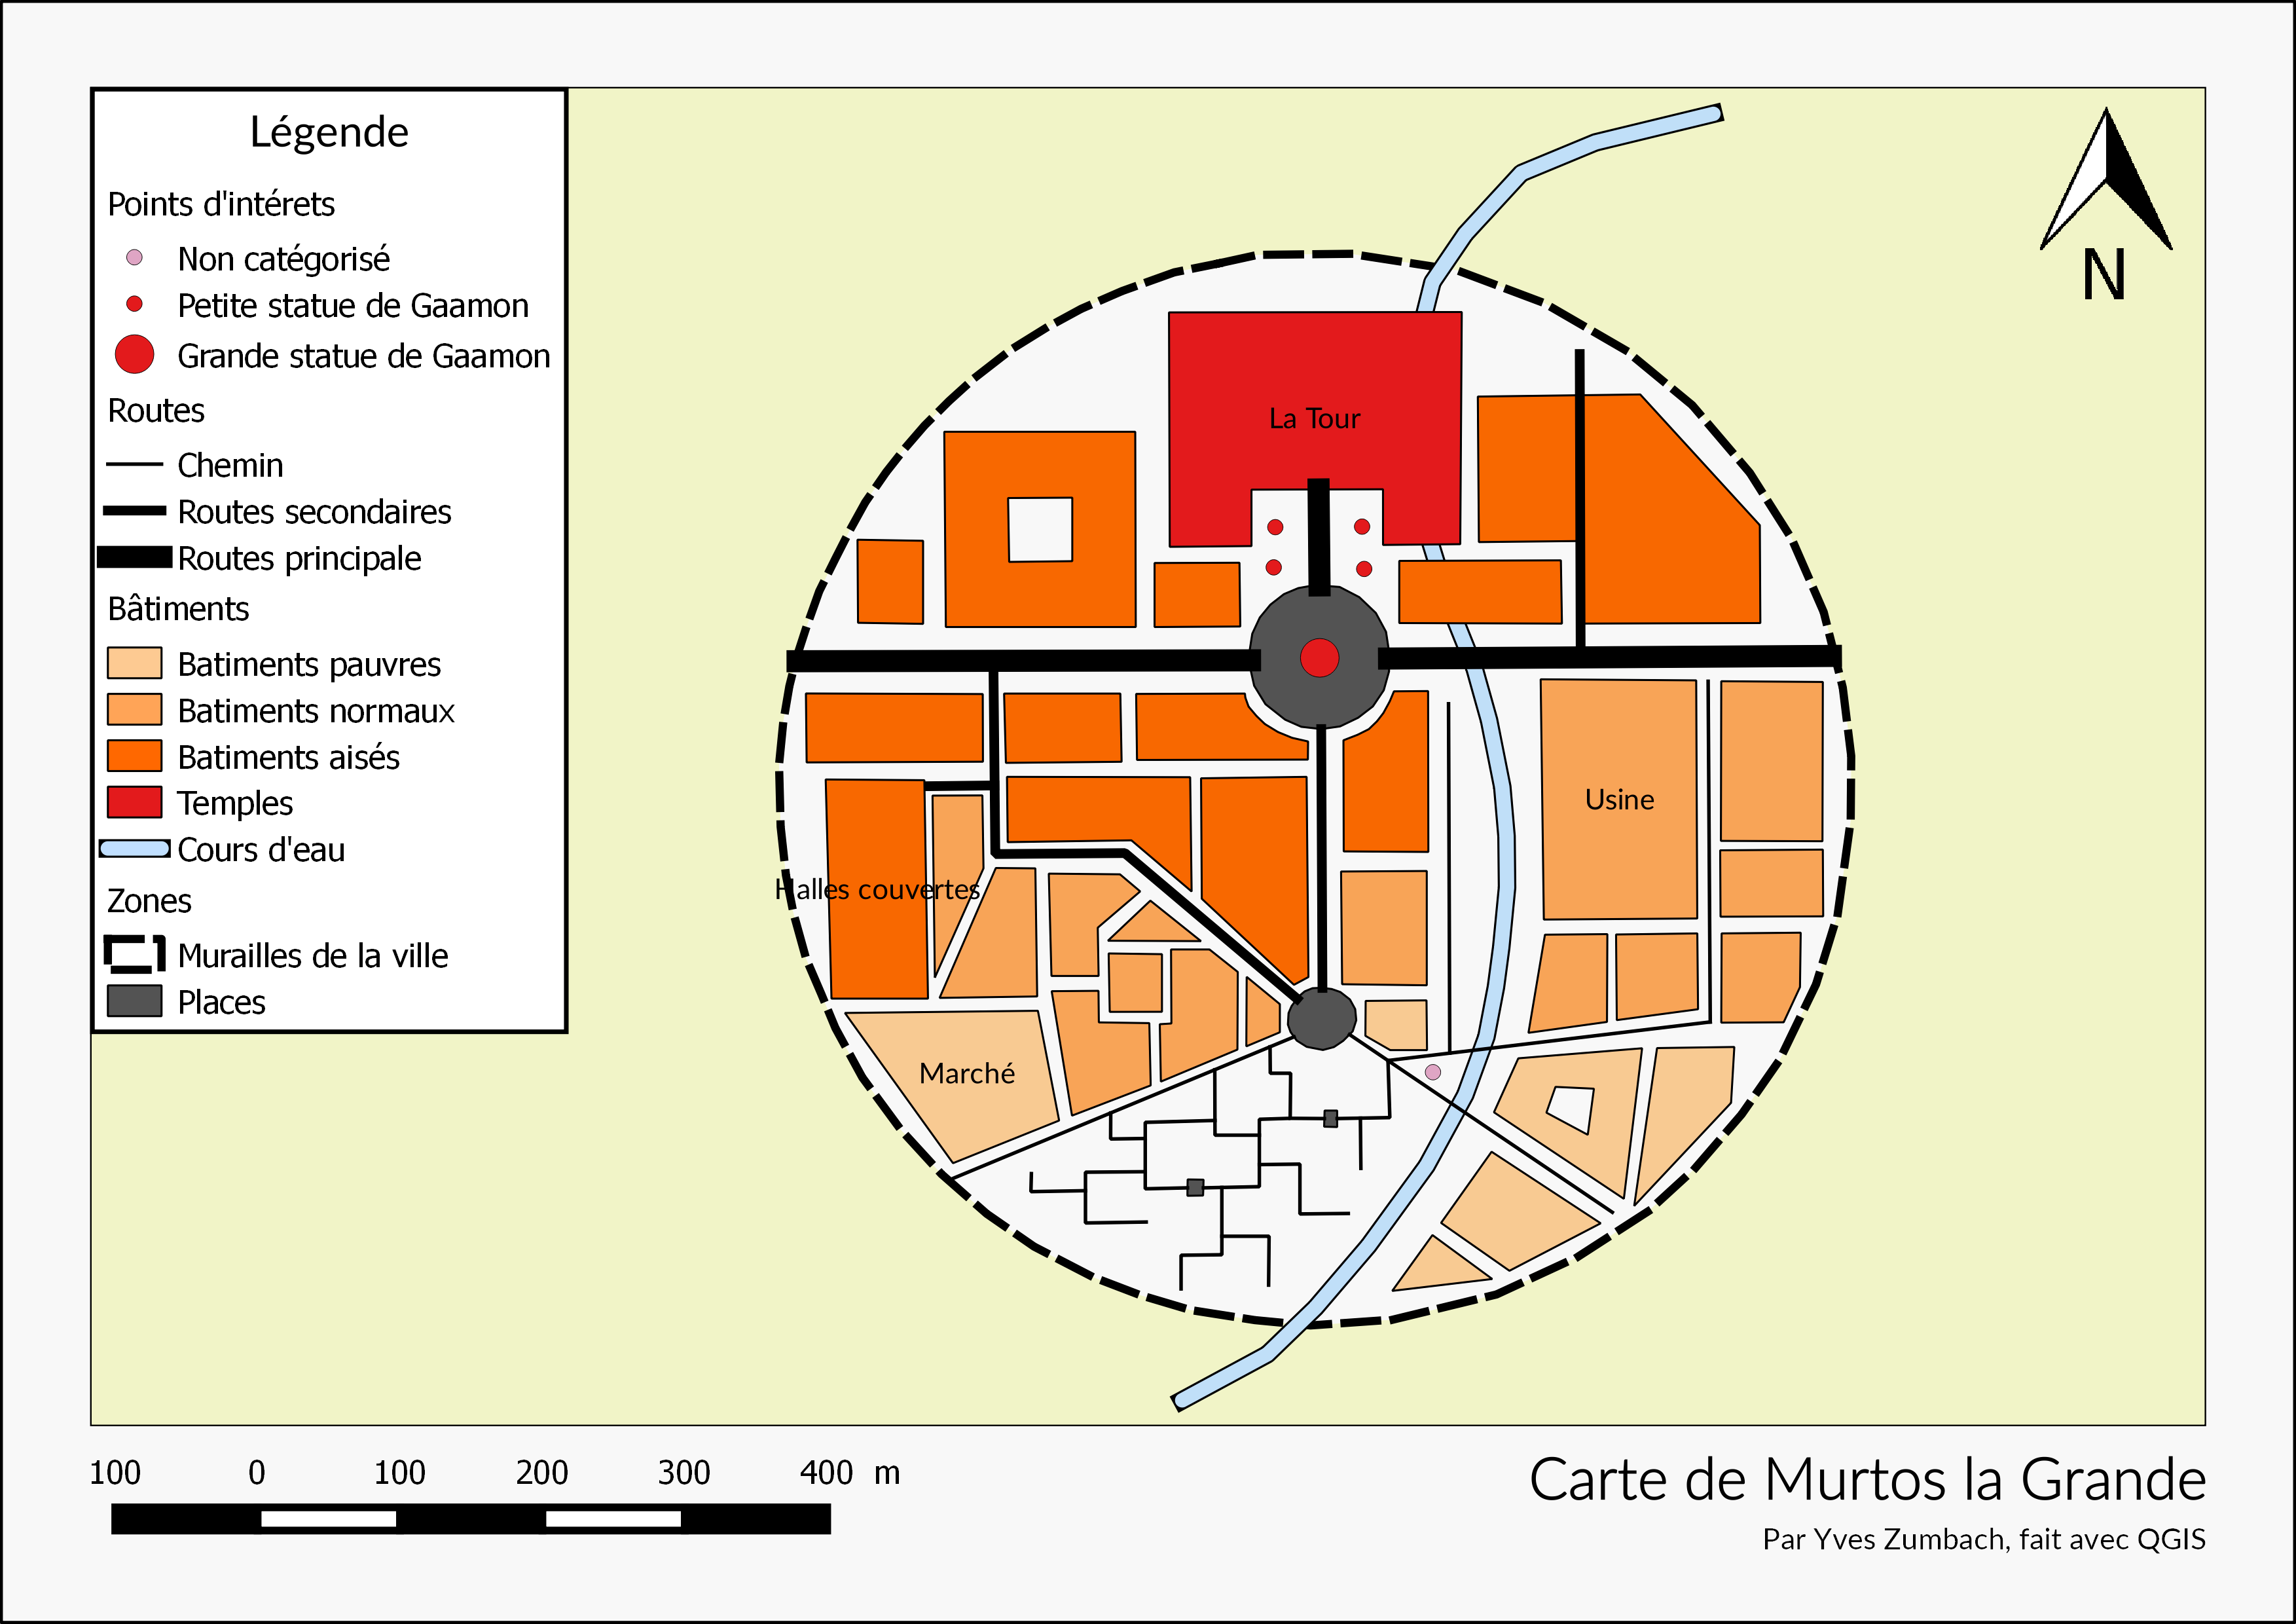
\includegraphics[width=\textwidth+2cm]{images/Monde/carteVille.png}
	\caption{Plan de Murtos la Grande (réalisé à l'aide du programme Quantum GIS)}
	\label{fig:murtosLaGrande}
\end{figure}

\subsection{La ville}
La ville est donc le bastion de la race humaine, l'empire de Lord Gaamon. Son décor relève de l'univers steampunk (\textit{cf.} annexe \ref{app:steampunk}). Il s'agit d'un monde urbain de l'ère industrielle où l'horizon est rythmé par les cheminées des hauts fourneaux qui crachent leurs fumées nauséabondes et où la suie recouvre les architectures de métal et de verre. Cet environnement, métaphoriquement, représente l'utilisation abusive de la technologie. C'est aussi la haine envers la Nature, sa négation totale. (plan de Murtos à la figure \ref{fig:murtosLaGrande})

\subsubsection{Redel, le quartier pauvre}
Les deux premiers niveaux du jeu (\textit{cf.} section \ref{sec:premierActe}) se déroulent dans le quartier pauvre, nommé Redel (\textit{cf.} cartes \ref{fig:murtosLaGrande} et \ref{fig:carteQuartierPauvre}). Il se situe à l'extrême sud de \nomVille. C'est le quartier le plus sale, où vivent les gens les plus pauvres.

Le coin sud-est du quartier est occupé par une énorme usine gouvernementale. L'accès à cette dernière est formellement interdit et des gardes surveillent en continu son entrée. De plus, elle crache sur le quartier des fumées toxiques, particulièrement malsaines à respirer.

\subsubsection{Un \enquote{bastion vert}}
Les dernières personnes à croire en la Nature habitent les maisons les plus isolées, au sud de Redel (\textit{cf.} carte \ref{fig:carteQuartierPauvre}). Ces gens cachent cependant leur croyance, de peur d'être persécutés. N'ayant plus vu une plante depuis des années, ils commencent à oublier ou à sombrer dans la superstition.

Un des trois sanctuaires de la Nature, celui de Tia, est caché dans ce quartier. Pour y accéder, un passage secret existe dans la maison située juste au nord de ce jardin caché. Cette dernière est habitée par Maïnin, un vieil homme sage qui a gardé l'esprit clair et lucide.


\subsection{Religion humaine}
La religion humaine est, à l'image de la ville, corrompue. Elle prône le bonheur par l'aisance matérielle, la richesse et la consommation. C'est même une apologie de la consommation --- si possible inutile --- que soutient ce dogme. De plus, les prêtres professent que l'argent ne s'acquiert que par le travail. Gaamon utilise la religion pour asservir les masses et motiver un travail acharné dans ses usines. Le symbole de ce culte possède une forme très caractéristique (\textit{cf.} figure \ref{subfig:accedeBonheur}) qui s'emboite avec l'icône de Gaamon pour représenter la collusion Religion--État. Quelques images de propagande que l'on peut trouver placardées sur les murs de la ville sont données à la figure \ref{fig:propagandeReligion}.

\vspace*{1cm}
\begin{figure}[ht]
	\subfloat[\label{subfig:accedeBonheur}Accède au Bonheur!]{
\includegraphics[width=.48\linewidth]{images/Monde/accedeAuBonheur.png}}
	\hspace*{.04\linewidth}\subfloat[Consommer pour la santé]{
\includegraphics[width=.48\linewidth]{images/Monde/consommerPourSante.png}}
	
	\subfloat[La Richesse c'est le Bonheur!]{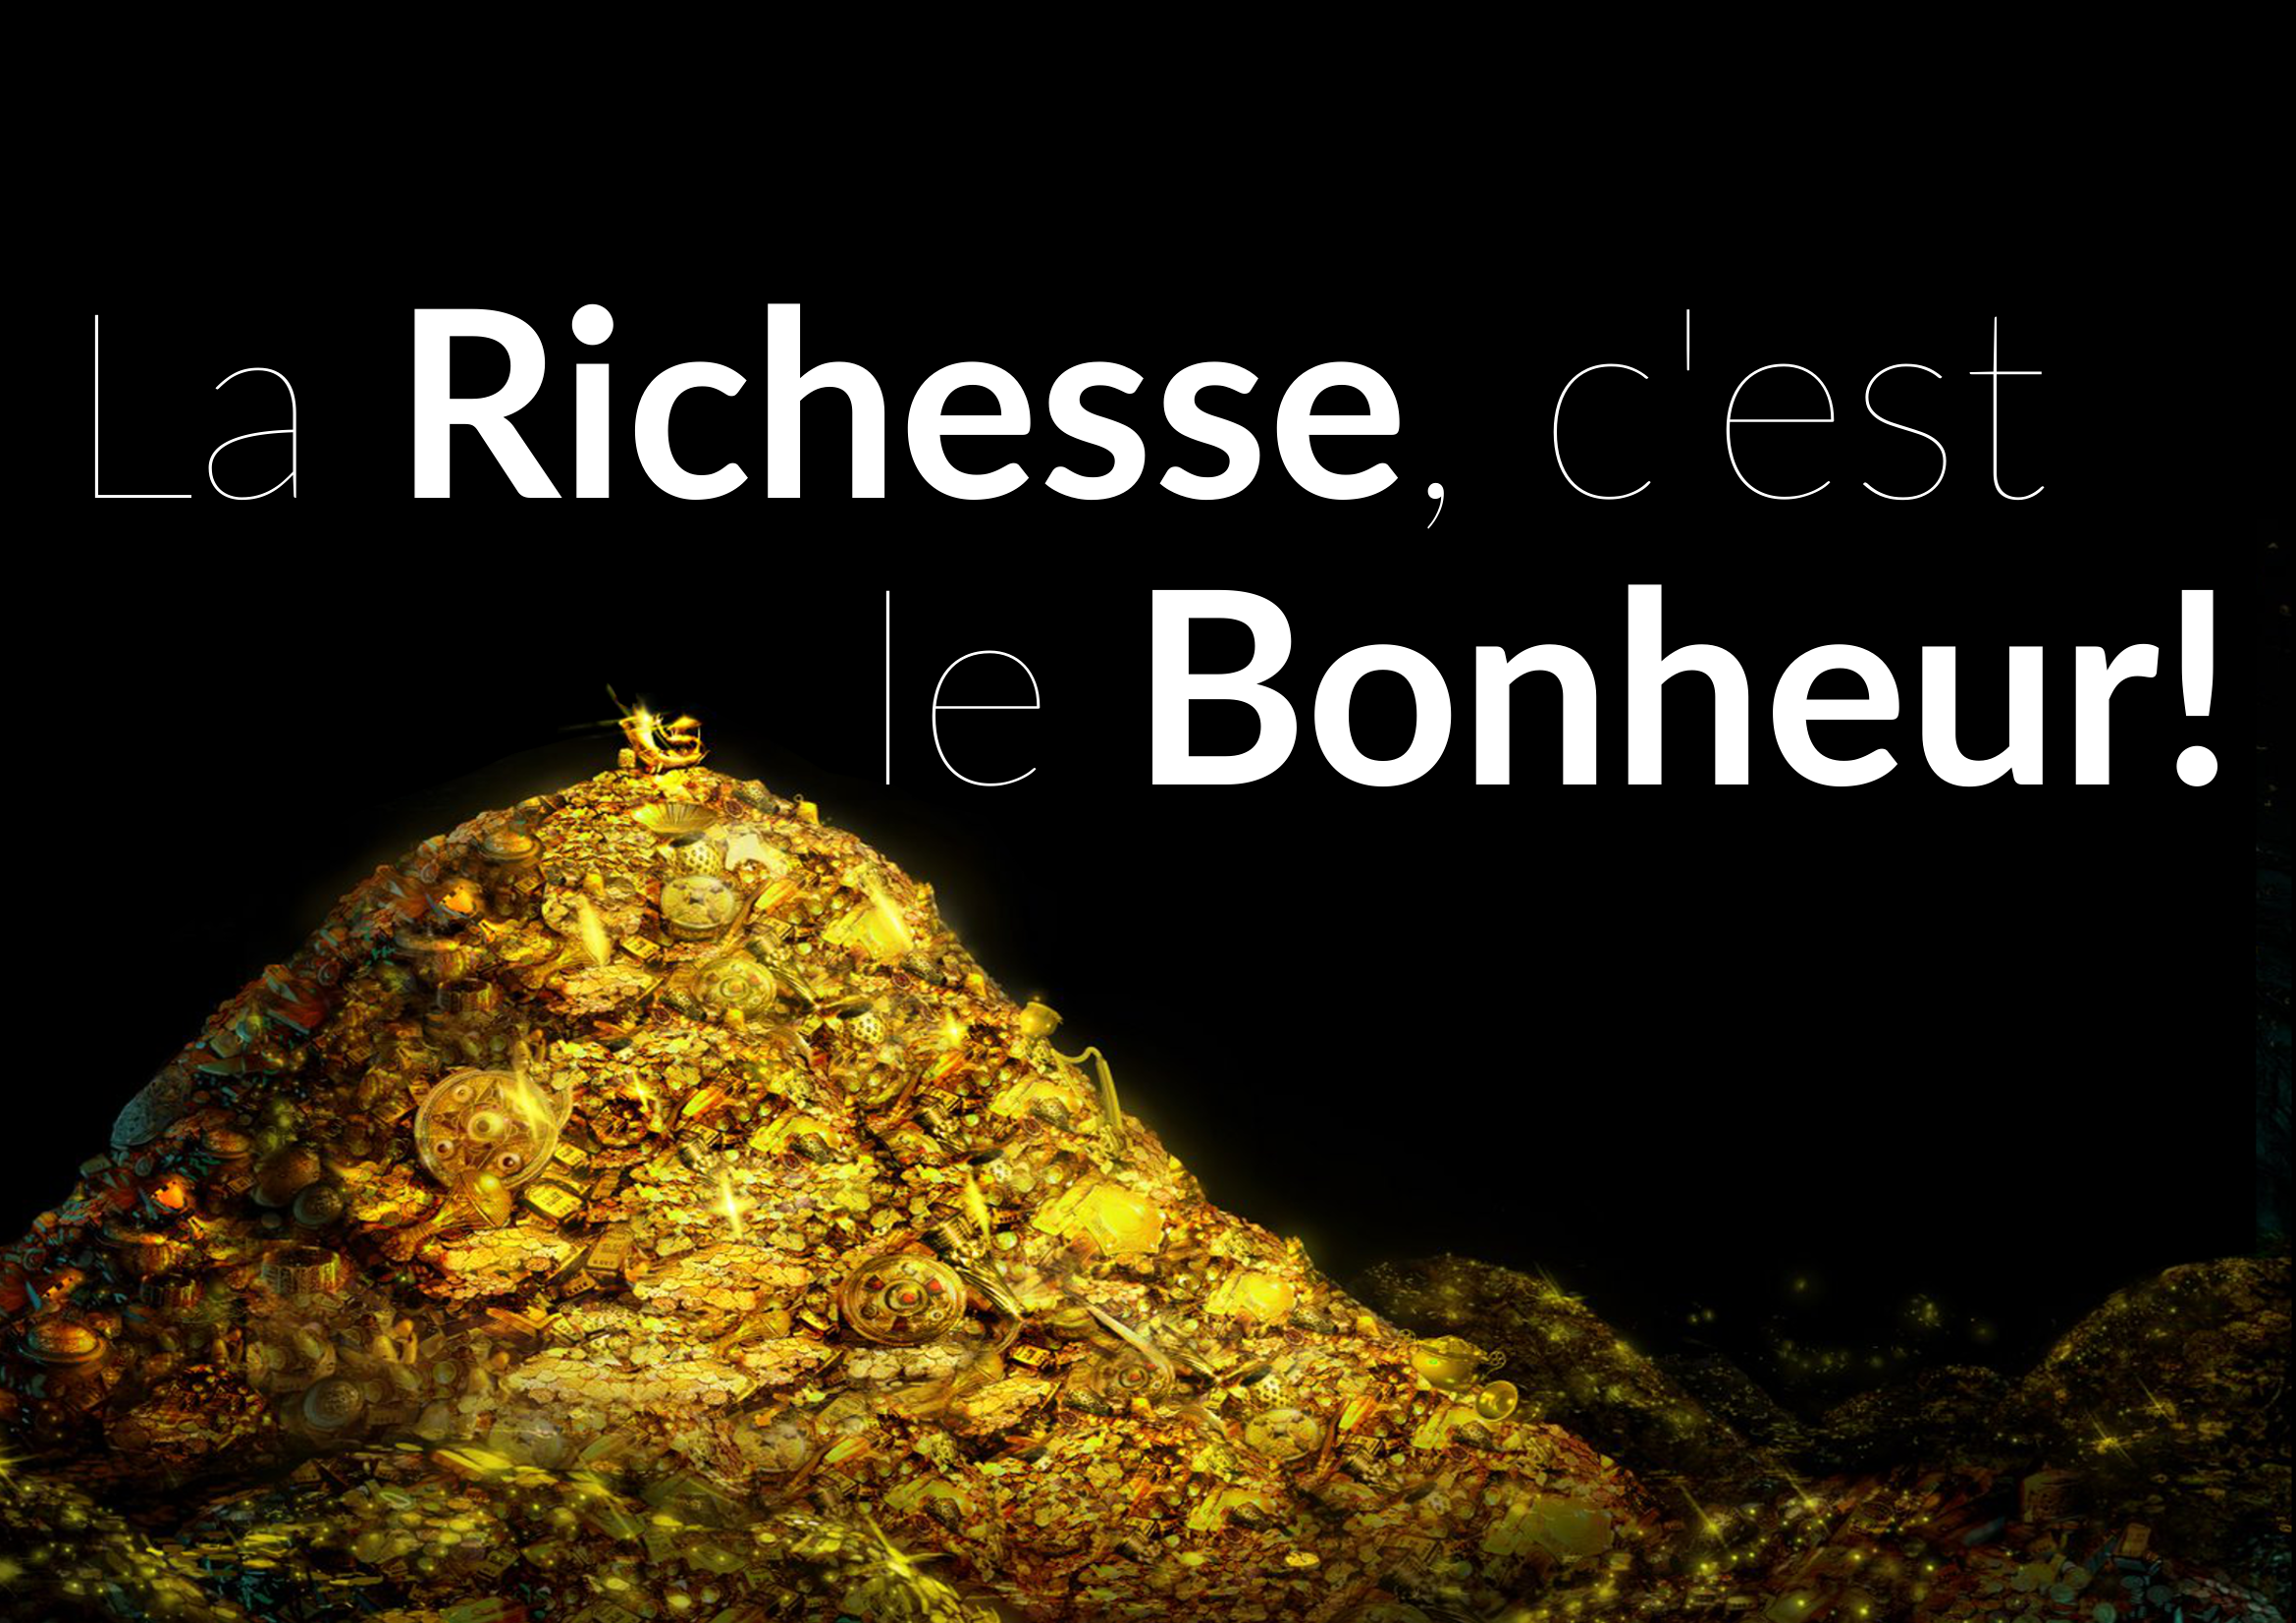
\includegraphics[width=.48\linewidth]{images/Monde/RichesseBonheur.png}}
	\hspace*{.04\linewidth}\subfloat[L'aisance matérielle par le travail]{
\includegraphics[width=.48\textwidth]{images/Monde/travailRichesse.png}}
	\caption{\label{fig:propagandeReligion}Propagande religieuse}
\end{figure}


\subsection{Propagande gaamoniste}
Gaamon utilise également les affiches, parmi d'autres vecteurs, pour répandre ses idées. Un aperçu en est donné à la figure \ref{fig:propagandeEtatique}. Les images \ref{subfig:gaamonSauverNature} et \ref{subfig:eliminezTouteNature} répandent les volontés \enquote{anti-naturelles} étatiques. Les figures \ref{subfig:industrialisationPourPuissance} et \ref{subfig:electricite} défendent l'industrialisation massive du peuple humain pour la puissance qu'un tel apport fourni.

\begin{figure}[ht!]
	\subfloat[\label{subfig:gaamonSauverNature}Gaamon pour vous sauver de la Nature]{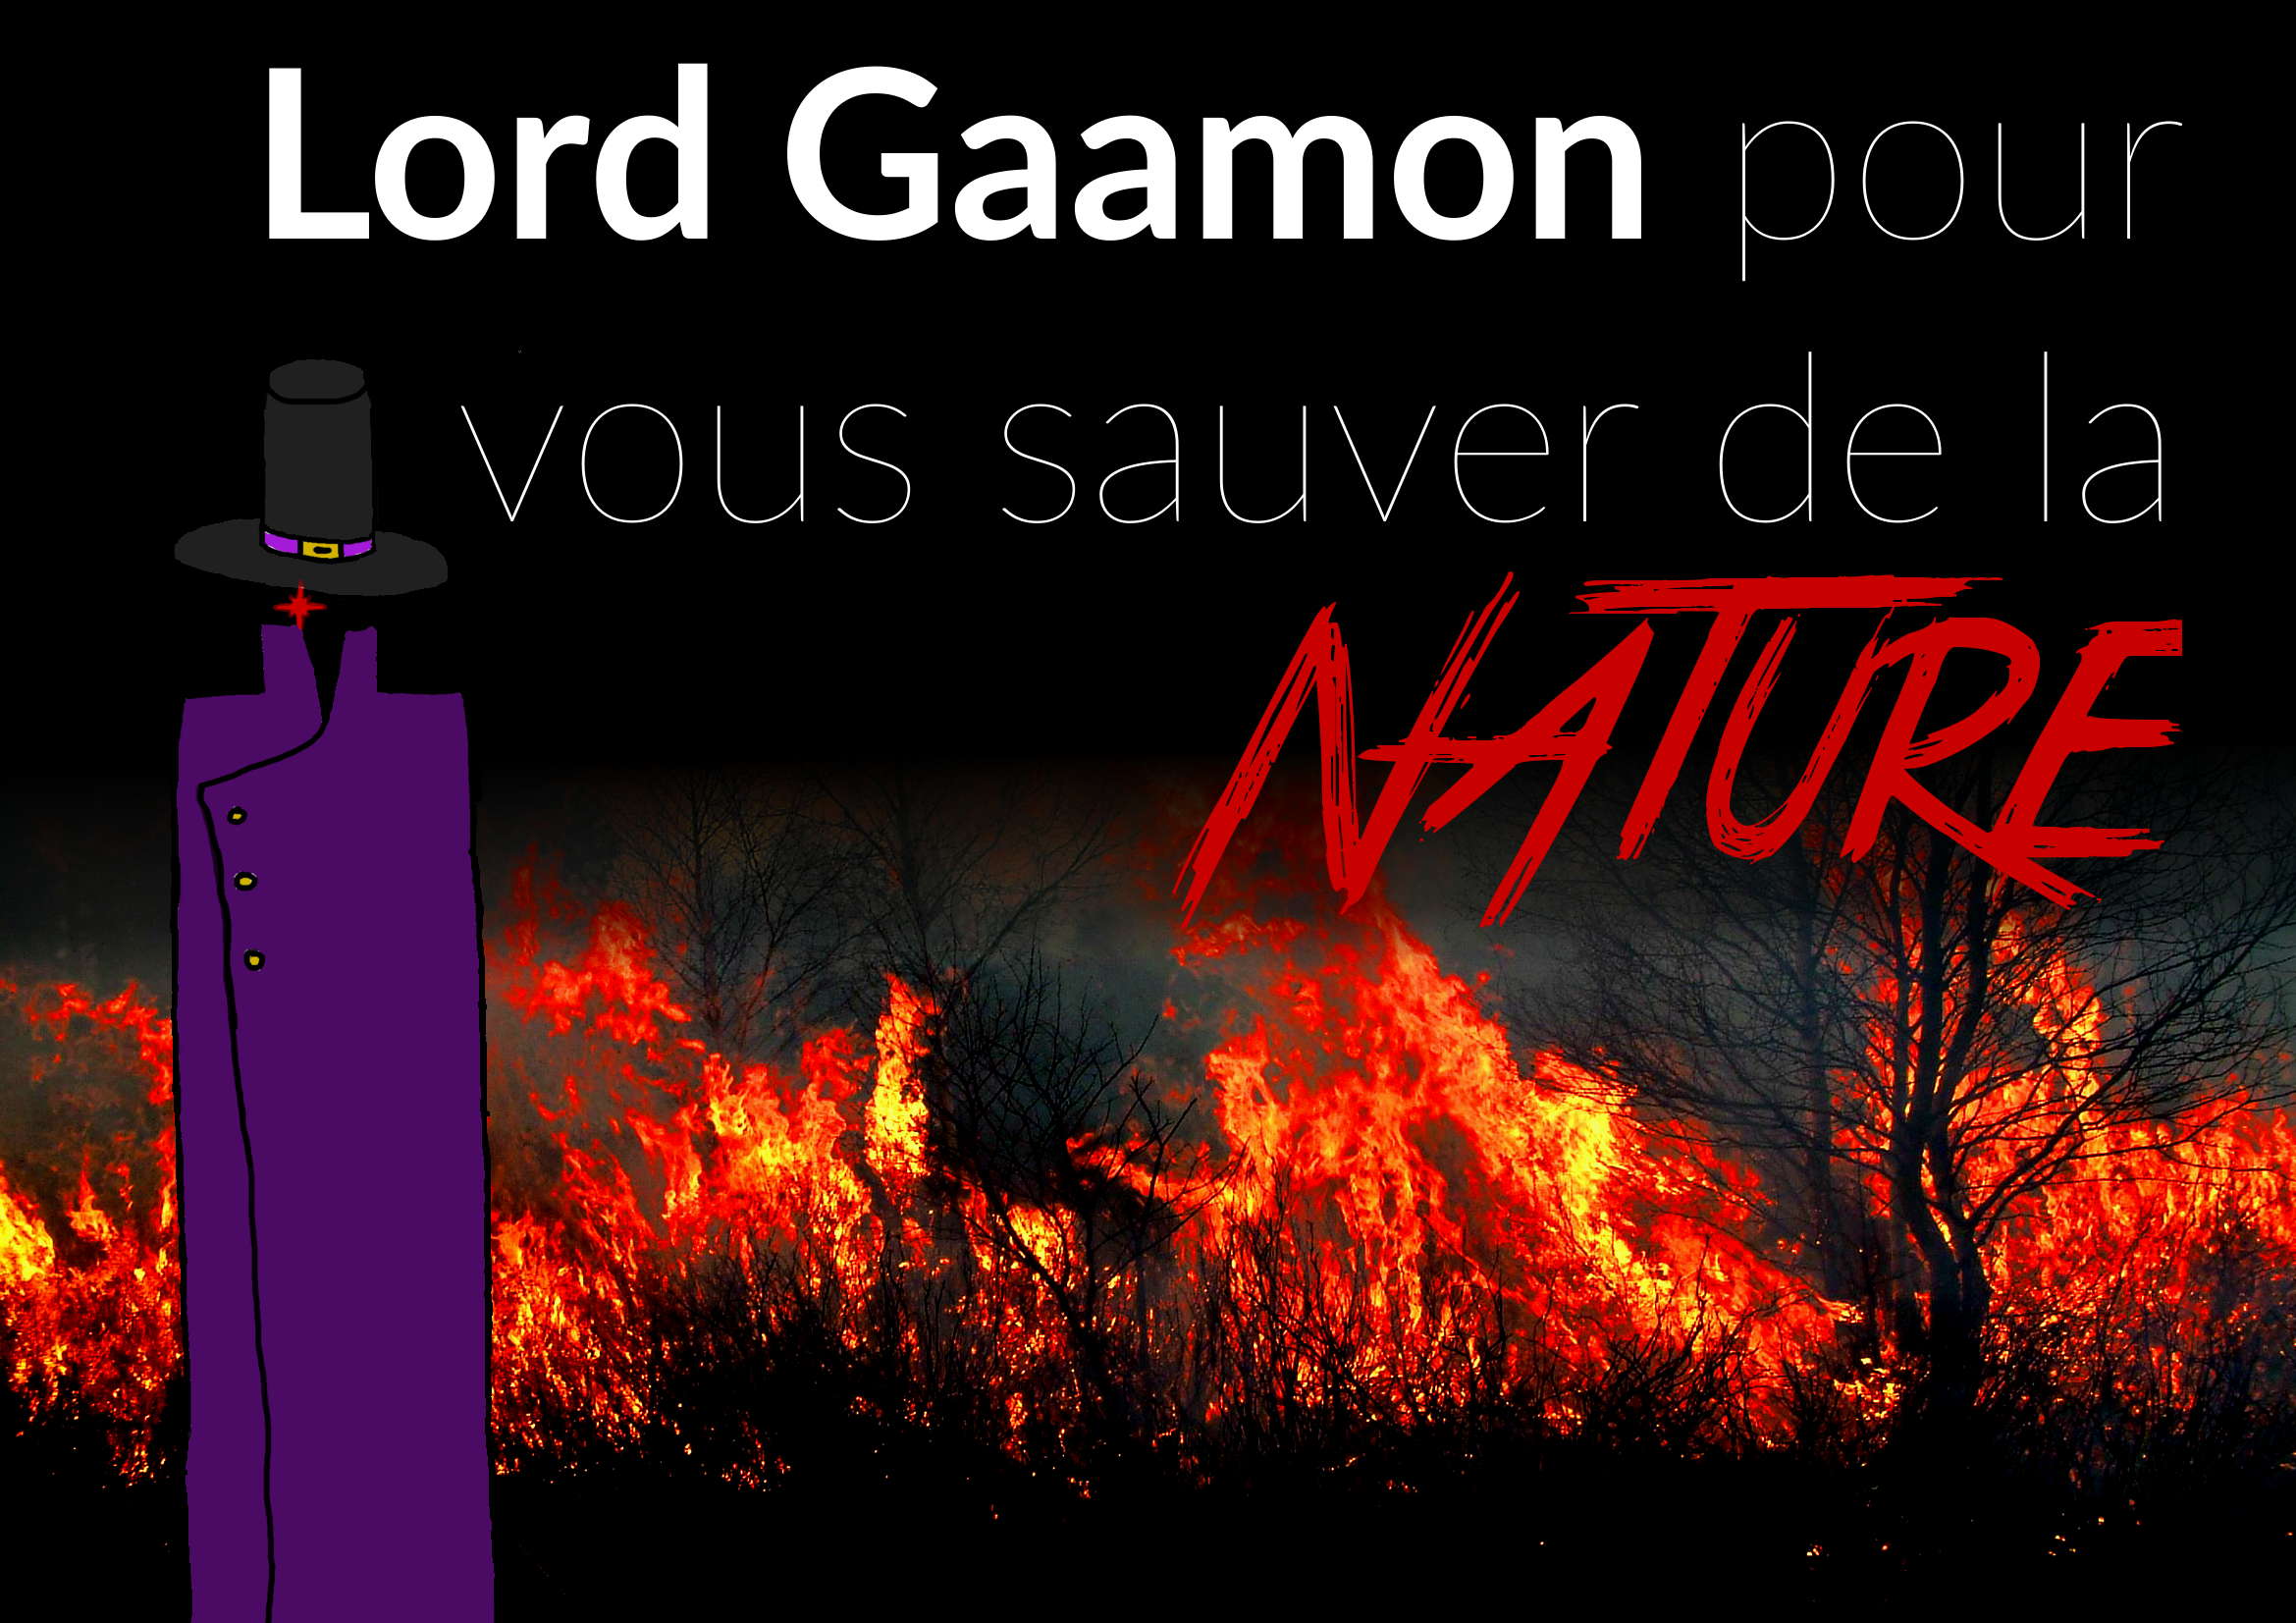
\includegraphics[width=.48\linewidth]{images/Monde/gaamonPourVousSauverNature.png}}
	\hspace*{.04\linewidth}\subfloat[\label{subfig:eliminezTouteNature}Éliminez toute Nature]{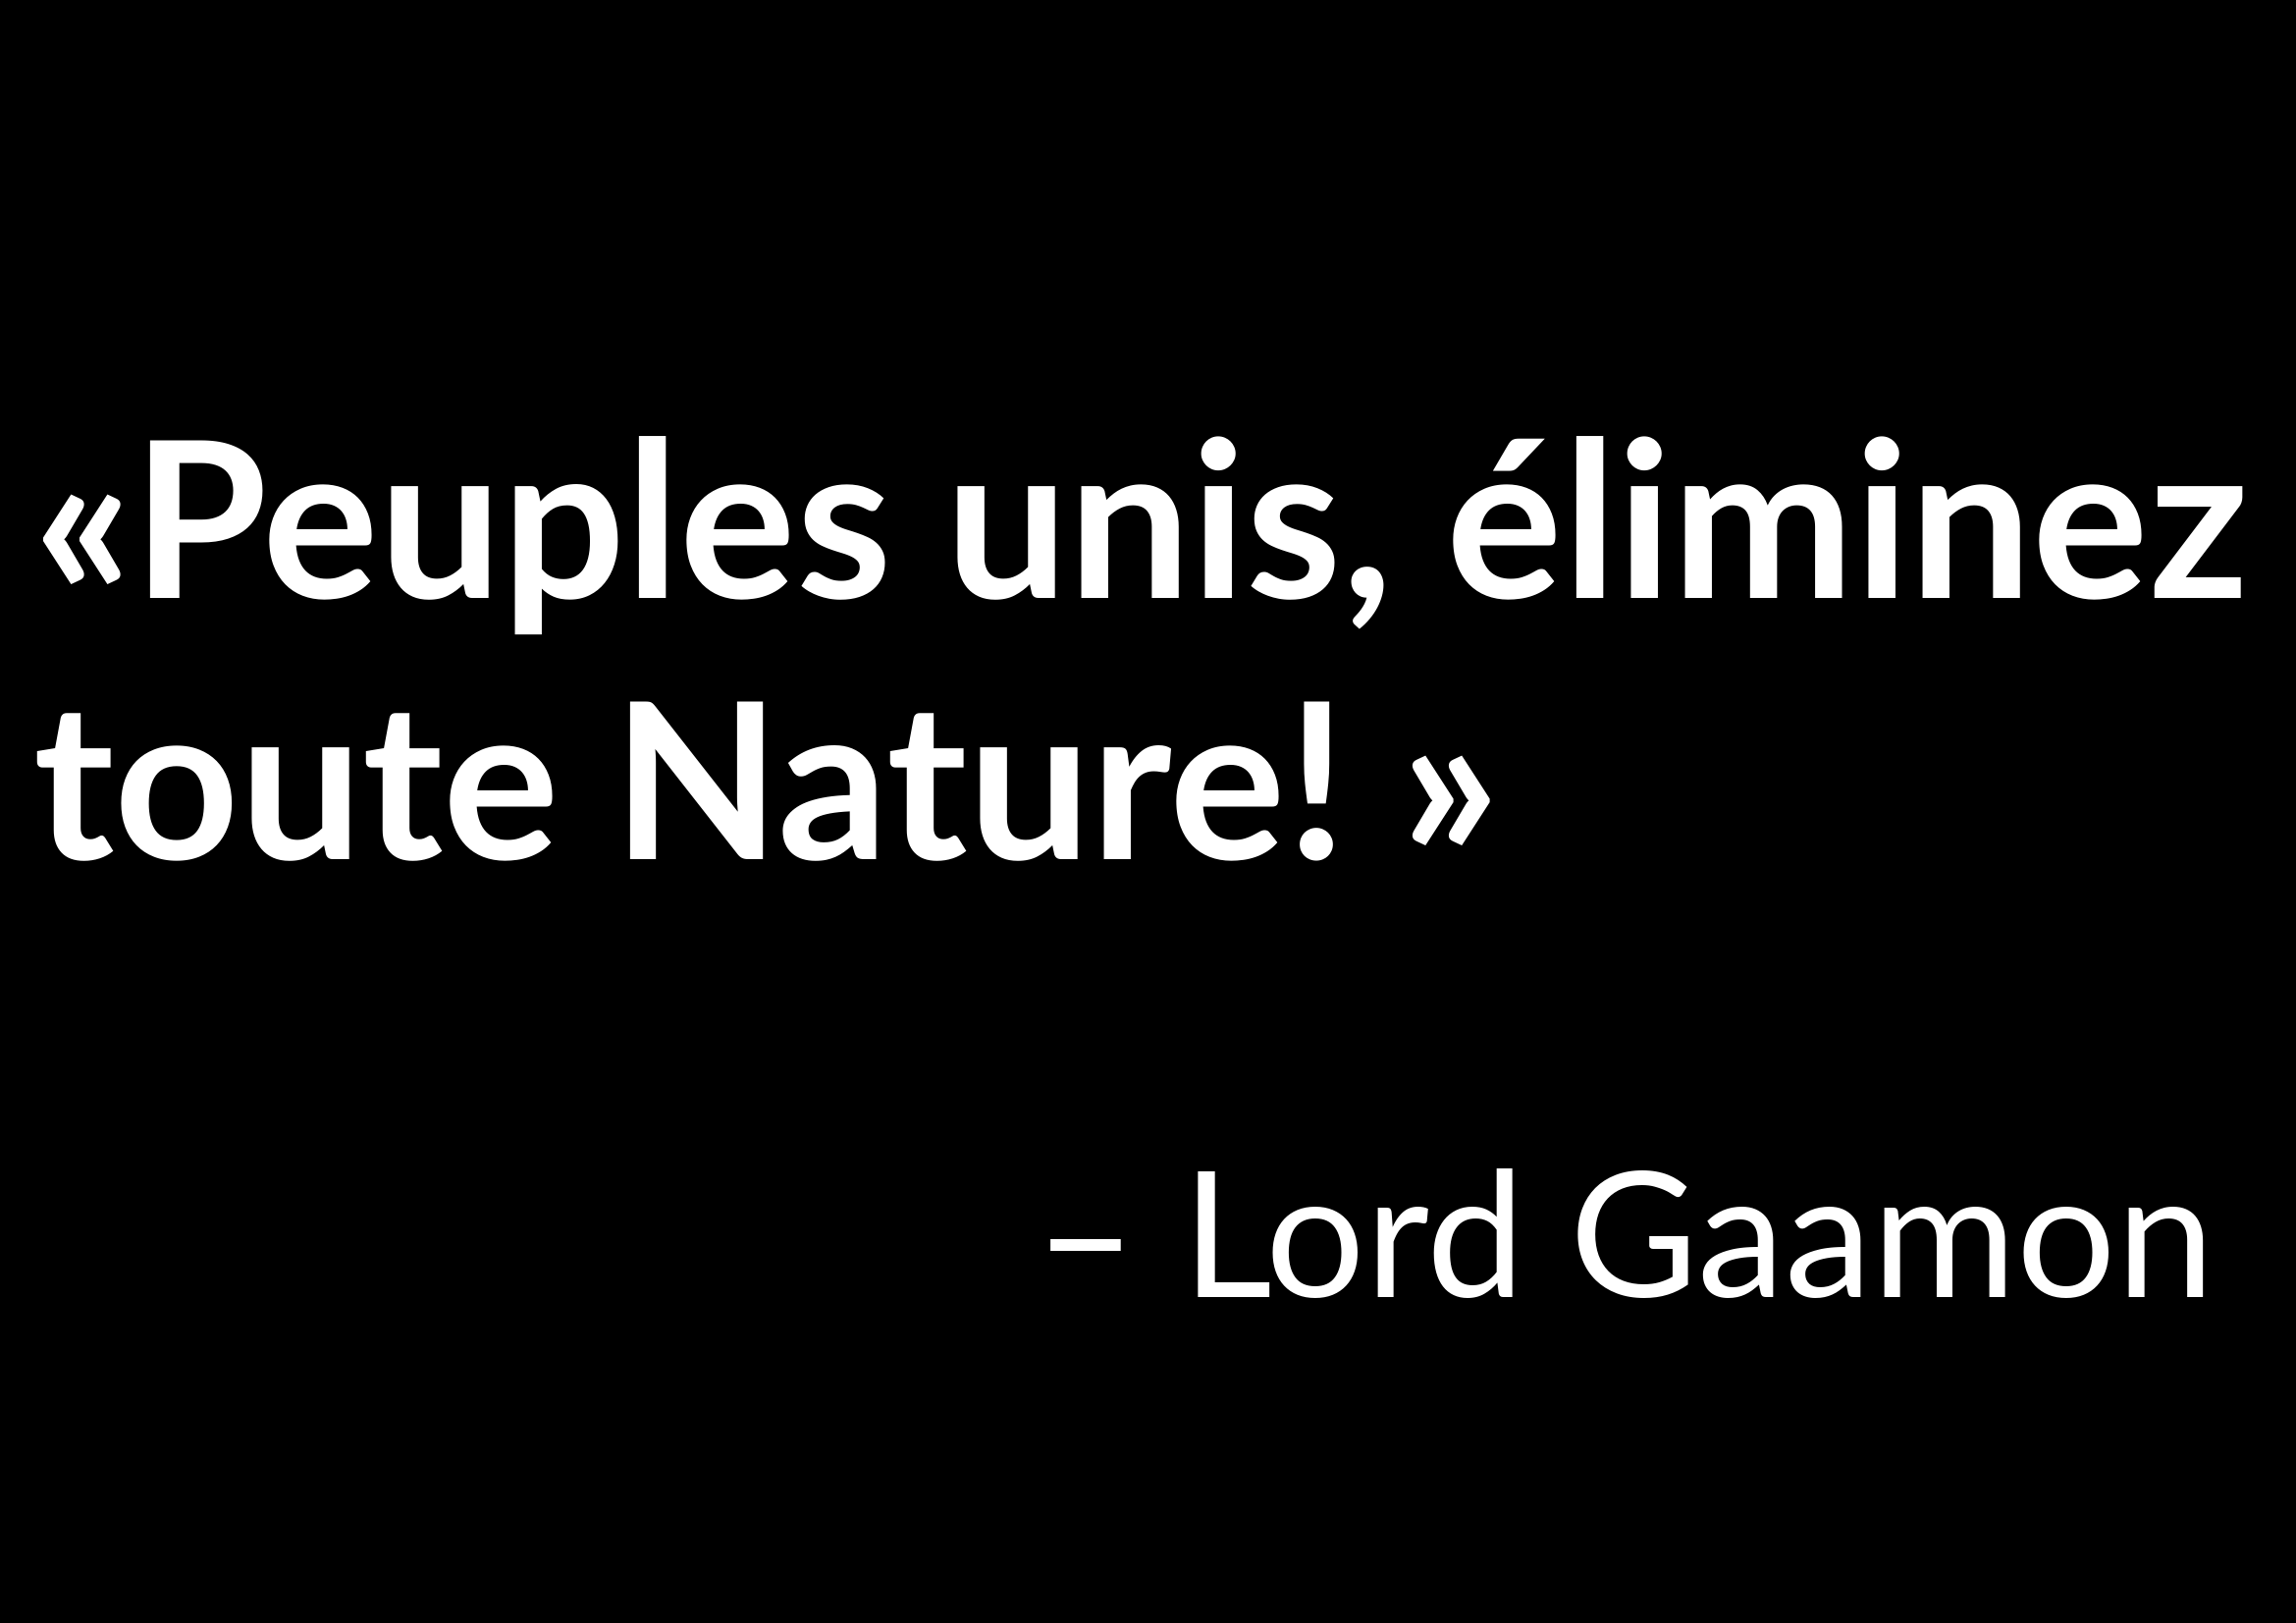
\includegraphics[width=.48\linewidth]{images/Monde/eliminezTouteNature.png}}
	
	\subfloat[\label{subfig:industrialisationPourPuissance}L'industrialisation pour la Puissance]{
\includegraphics[width=.48\textwidth]{images/Monde/industrialisationPourPuissance.png}}
	\hspace*{.04\textwidth}\subfloat[\label{subfig:electricite}Électricité]{
\includegraphics[width=.48\linewidth]{images/Monde/light.png}}
	\caption{\label{fig:propagandeEtatique}Propagande étatique}
\end{figure}



\section{Les \nomNaturels s}

\subsection{Leur histoire}
\label{sec:histoireNaturels}
Les \nomNaturels s étaient, par le passé, le peuple le plus brillant et le plus avancé d'\nomUnivers. Ils avaient trouvé une source d'énergie formidable, l'énergie verte, qui leur permettait de vivre heureux et prospères. L'extraction de cette ressource naturelle était un processus compliqué que seuls les shamans de l'énergie maîtrisaient (\textit{cf.} section \ref{sec:energies}). Grâce à cette source, leurs cités étaient magnifiques, leurs manières connues pour leur raffinement et leur art reconnu pour sa délicatesse.

Ce peuple jouissait d'une prospérité jusque-là sans égale dans l'histoire et répandait sa sagesse, ses connaissances et son amour de la nature de par le monde. L'ascension au pouvoir de Gaamon marqua la fin de cette période; afin d'empêcher la propagation d'un idéal qui mettait la Nature au centre des préoccupations, il fit assassiner les prêtres de l'énergie. Les \nomNaturels s se retrouvèrent subitement privés de leur source vitale --- l'énergie verte --- sans protection et virent leur civilisation s'effondrer brutalement.

Les \nomNaturels s vivent maintenant reclus sur de hauts plateaux, cachés de la haine ainsi que des persécutions de Gaamon et rêvent de leur gloire passée. Si leur idéologie d'amour envers la Nature perdure, leur civilisation décline inexorablement.



\section{Énergies}
\label{sec:energies}
Les énergies sont un élément clé de ce monde. Elles déterminent quels peuples survivront et lesquels disparaîtront. C'est un parallèle de notre dépendance à l'énergie. En effet, on ne peut plus imaginer aujourd'hui vivre sans électricité. À \nomUnivers, les sources d'énergie sont diverses et représentatives des peuples.

\subsection{Humains}
Chez les Humains, l'énergie est tirée du charbon pour créer de la vapeur et de l'électricité. C'est une source très polluante. La couleur qui lui est attribuée est le rouge du feu des hauts fourneaux et le noir de la fumée qui remplit le ciel de \nomVille. Elle fait partie intégrante du Steampunk, caractéristique de ce peuple.

\subsection{\nomNaturels s}
\label{sec:energieTelurans}
À l'inverse, les \nomNaturels s ont exploité l'énergie des arbres, appelée énergie verte. Les plantes fournissaient un apport énergétique et, en contrepartie, les \nomNaturels s portaient une attention toute particulière à leur santé, reproduction, protection et longévité. Une symbiose existait entre les \nomNaturels s et la Nature, un équilibre grandement profitable autant pour l'un que pour l'autre. L'énergie verte était extraite dans la grande salle, dont l'accès était réservé aux grands shamans de l'énergie, seules personnes à pouvoir maîtriser son fonctionnement complexe. Si ce secret était aussi bien gardé, c'est que cette énergie extrêmement puissante, extraite en trop grandes quantités, pouvait causer la mort de milliers d'arbres et animaux. Et un tel cas de figure était à craindre fortement, car la Nature se serait alors retournée contre ceux qui auraient abusé de ses ressources et, dans sa fureur, aurait annihilé des peuples entiers. Les \nomNaturels s, craignant une pareille situation, s'en étaient prémunis en cachant les mécanismes de la grande salle pour ne les révéler qu'aux seuls élus, les shamans.

Cette énergie pouvait également être maîtrisée, dans une moindre mesure, à titre personnel. Les personnes dotées de telles capacités pouvaient alors lancer des \enquote{sorts}. Ceci est un des éléments clé du gameplay (\textit{cf.} section \ref{sec:sorts}). On pourrait comparer l'énergie verte à de la magie mais cela n'est que partiellement correct: l'énergie verte n'est ni illimitée, ni gratuite. L'utiliser de façon disproportionnée signifie tuer toute vie alentour. Et si la Nature est généreuse elle peut aussi refuser de donner son bien, voire punir ceux qui en abusent. Il est également possible de l'extraire de soi-même, mais une fois de plus, la réalisation d'une telle opération est dangereuse car elle peut causer la mort de l'exécutant.

Depuis la disparition mystérieuse des shamans (\textit{cf.} section \ref{sec:histoireNaturels}), les \nomNaturels s ont perdu le secret de l'énergie verte. Ils utilisent donc les énergies hydraulique et éolienne, facilement disponibles dans les montagnes où ils vivent. Elles sont cependant bien moins puissantes que l'énergie verte et ne leur permettent de loin pas les miracles qu'ils pouvaient accomplir avec la première.



\section{Bestiaire}
\label{sec:Bestiaire}

\begin{wrapfigure}[12]{r}{.3\textwidth}
	\vspace*{-.8cm}
	\center
	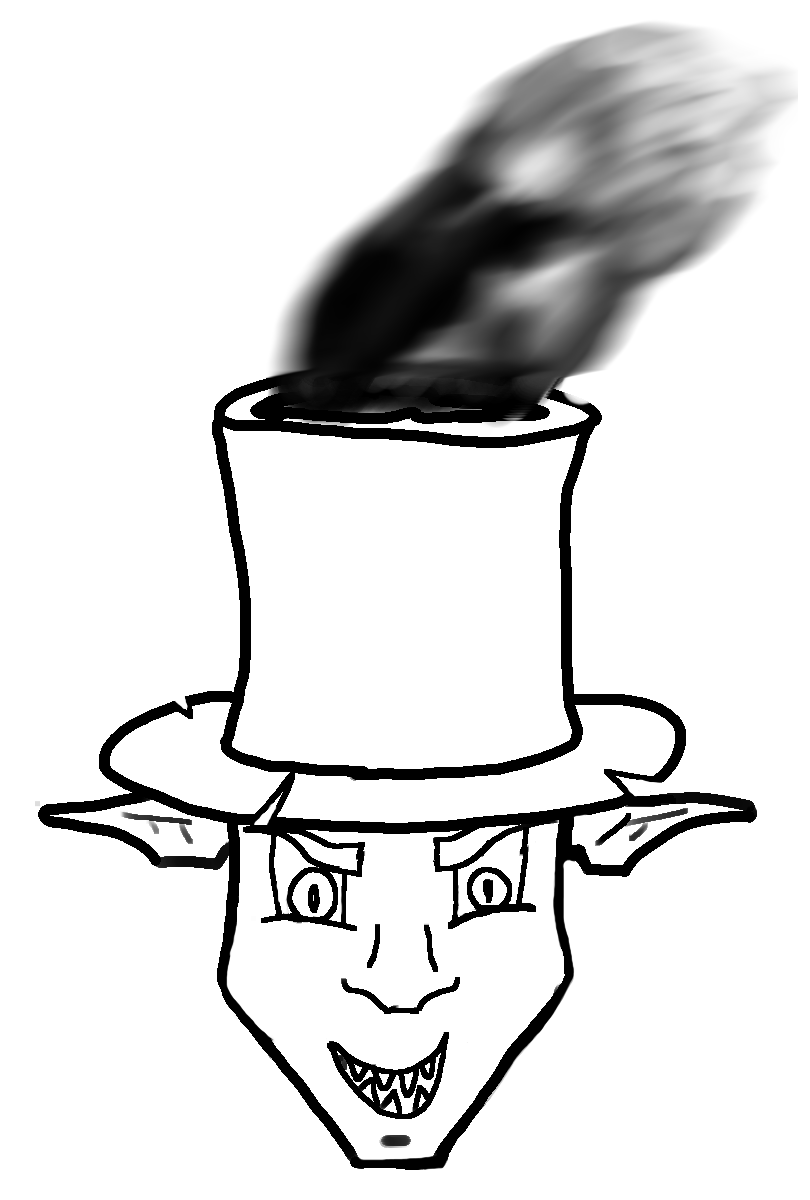
\includegraphics[width=.3\textwidth]{images/Monde/Gnobol.png}
	\caption{\label{fig:Gnobol}Gnobol}
\end{wrapfigure}
Du point de vue des genres, le monde d'\nomUnivers\ est un croisement entre la science-fiction et la \anglicisme{Fantasy}, car il est peuplé de créatures féériques et rempli des machines futuristes de Gaamon.

\subsection{Créatures humaines}
\subsubsection{Gnobols}
\label{sec:Gnobols}
Les sbires de Gaamon sont des créatures nommées \textit{Gnobols}. Il existe beaucoup de variantes de la créature \enquote{de base}. Certains pourraient être équipés d'une armure, d'autres d'un arc, d'un fusil, de bombes fumantes ou encore de sifflets d'alarme. Ils sont en revanche tous équipés d'un chapeau duquel une fumée noire s'échappe.

Ces créatures sont en fait des machines inventées par Gaamon et produite à la chaine dans les usines de Murtos. (\textit{cf.} figure \ref{fig:Gnobol})

\subsection{Personnalisation de la Nature}
\label{sec:personnalisationNature}
Dans l'univers d'\nomUnivers, la Nature est personnalisée par trois esprits, chacun représentatif d'un aspect de la Nature. La caractéristique qu'il personnifie définit leur apparence:

\begin{table}[ht!]
	\newlength{\tableLength}
	\setlength{\tableLength}{\textwidth+2.34cm}
	
	\hspace*{-2.34cm}
	\begin{tabu} to \tableLength {l l X X X l}
		\rowfont{\fontspec{Lato Heavy}\selectfont\leavevmode\color{white}}
		\rowcolor{mainColor}
		& Esprit & Description & Mots-clé & Apparence & \\
		& Leo & Il est la destruction renouvelatrice, à la fois créateur et destructeur, de son chaos naît la vie & Massif, sans distinction, abrupt, rapide, mort génératrice de vie & Golem, de pierre et de lave en bas, de pierre et d'eau en haut, avec un duvet de plante sur les épaules & \\
		& Tamund & Il est l'intelligence aveugle, l'évolution lente & Évolution, lent, ciblé, mort des plus faibles & Grand séquoia aveugle & \\
		& Tia & Elle est la vivacité sauvage et profite parfois sans pitié & Sauvage, vif, rapide, profiteur, sans-pitié, survie du plus adapté et mort des plus faibles & Écureuil avec des runes sur le dos & \\
	\end{tabu}
	
	\caption{Les trois esprits et leurs caractéristiques}
\end{table}

\begin{figureWithNotes}[p]
	\center
	\thisfloatpagestyle{empty}
	\captionsetup{format=myformat}
	\hspace*{-3.5cm}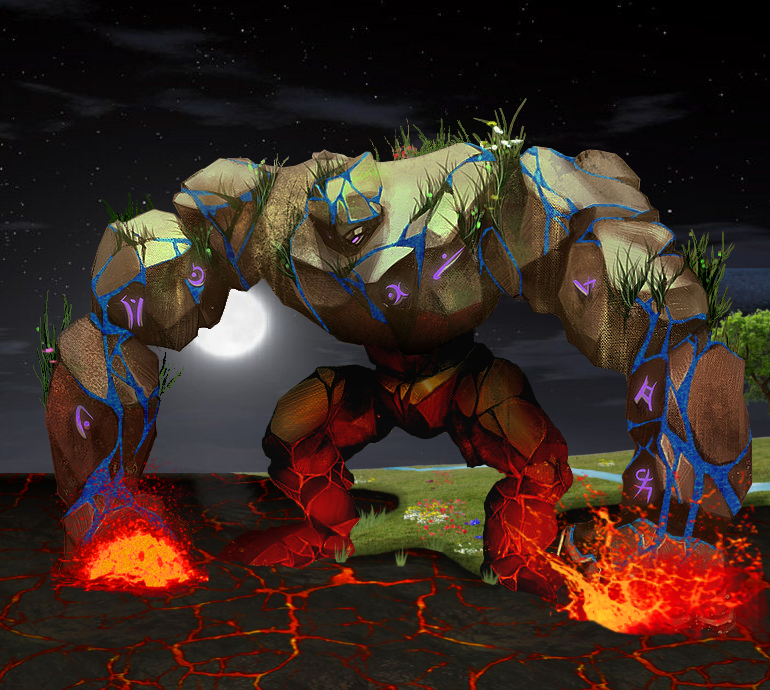
\includegraphics[width=\paperwidth-\myHorizontalTotalMargins]{images/Monde/Leo/Leo.png}
	\caption{Exemple de ce que pourrait être l'apparence de Leo,\\basée sur le travail original de Sinto-risky {\cite{StoneGolem_Sinto-risky}}}
	%\spewnotes
\end{figureWithNotes}



\chapter[Gameplay, ou la façon de jouer]{Gameplay,\\ou la façon\\de jouer}
\printMiniToc

\label{chap:gameplay}

\normalInfo{Une question de vocabulaire}{Ce chapitre porte sur un sujet relativement technique et récent. L'univers du jeu vidéo étant principalement anglophone, le vocabulaire de ce domaine est composé de beaucoup d'anglicismes, tel \anglicisme{gameplay}. La langue française n'a pas encore eu le temps de s'adapter. Pour cette raison, les anglicismes seront conservés et typographiés de \anglicisme{cette façon}.}

\section{Idée générale}
Ce jeu tente de promouvoir la paix et la résolution de problème par des solutions non-violentes. De ce parti pris découleront bien des aspects. Ainsi, le joueur sera \enquote{puni} s'il utilise ses armes, mais il est à noter qu'elles restent à disposition et peuvent être améliorées, tout comme d'autres items. C'est aussi une question qui est posée au joueur: quelle voie préfère-t-il utiliser? Pacifique ou brutale? Libre à lui de choisir, mais le jeu prend parti pour celle qui n'utilise pas la violence et répercute cela sur le score et certaines ressources.

\section{Mode de jeu \anglicisme{stealth}}
\anglicisme{Stealth}, en français, peut se traduire par furtif, discret, ruse ou encore dissimulation. Dans les milieux francophones, on parlera de jeu d'infiltration à la place de \anglicisme{stealth game}, cependant le sens n'est pas exactement le même. Ce terme, sans bonne traduction, représente bien le style de gameplay que l'on peut rencontrer dans \nomJeu. Le jeu défendant une approche pacifique, il est bien sûr hors de question de faire tirer le joueur sur ses ennemis ou de lui permettre de les démolir à coups de poings ou d'épée.

À la place, c'est un mode de jeu où il faut éviter les opposants, se cacher et rester discret, qui est privilégié. Un autre aspect développé est la résolution de problèmes, ainsi que la complétion de sous-quêtes. Finalement, on notera l'utilisation relativement répandue de puzzles\definition, qui nécessiteront de collecter des objets au fil des aventures pour pouvoir être résolus (\anglicisme{item collecting}). \cite{Stealthgame_}


\section{Les ressources}
Un élément important dans les jeux vidéos est représenté par les ressources. Des exemples de ressources sont l'argent, l'expérience (souvent abrégée XP), les munitions ou encore le mana qui représente une quantité de magie. Elles forment le \enquote{système économique}. La mesure dans laquelle les ressources sont disponibles peut faire toute la différence entre un bon et un mauvais titre: si elles sont trop abondantes, le jeu devient facile et les joueurs perdent leur intérêt, à l'inverse, si elles sont trop rares et difficiles à obtenir, le joueur se retrouve confronté à une difficulté trop importante et cesse de joueur par dépit.\cite{LevelUpTheGuidetoGreatVideoGameDesign_Rogers}

Dans \nomJeu, les ressources principales sont les suivantes:
\begin{itemize}
	\item Argent
	\item Énergie verte
	\item Coefficient de naturalité (score)
	\item Graines
\end{itemize}

L'énergie verte est une ressource un peu spéciale. Elle est décrite dans la section \ref{sec:energieTelurans} du point de vue de l'univers. Dans le jeu, elle est principalement utilisée pour lancer des sorts.

Les graines sont un autre type de ressource. Ces dernières sont rares et dispersées dans le jeu. Toutes les fonctionnalités décrites ci-après sont accessibles dans un menu séparé en 2D. Lorsque le joueur en découvre ou gagne une, il peut la planter. Il doit ensuite l'arroser et la nourrir. Plus il entretient la plante, plus elle grandit vite. Une fois adulte, la plante donne des fruits que le joueur peut cueillir, ce sont des bonus de vie, d'énergie verte, des ingrédients, etc. La quantité de fruits qui poussent dépend de l'attention apportée à la plante.

Les succès\definition\ font aussi partie du système économique mais pas au même titre que les ressources précédemment citées. En effet, on ne peut que gagner ou débloquer un succès, à l'accomplissement d'objectifs supplémentaires par exemple; impossible de les utiliser ou de les vendre ensuite. Ils font cependant partie du système de récompenses.

\begin{table}[ht!]
	\begin{tabu} to \textwidth {l X X[1.2] X[1.2] l}
		\rowfont{\fontspec{Lato Heavy}\selectfont\leavevmode\color{white}}
		\rowcolor{mainColor}
		& Ressources principales & Comment en gagner & Comment en perdre & \\
		& Argent & Compléter des quêtes,\newline Dans les coffres & Achats & \\
		& Énergie verte & Planter une graine,\newline Se régénère avec le temps & Utiliser la violence,\newline Lancer un sort & \\
		& Coefficient de naturalité & Faire preuve de naturalité,\newline Compléter des sous-quêtes & Utiliser la violence & \\
	\end{tabu}
	\caption{Gestion des ressources principales}
\end{table}

\section{Les sorts}
\label{sec:sorts}
Les sorts sont les principaux outils mis à la disposition du joueur.

Dans l'univers d'\nomUnivers, pour pouvoir lancer un sort, il faut posséder, le totem qui lui est associé. Ces totems se présentent sous la forme de petits grigris. Les esprits sont les seules créatures qui peuvent offrir de tels artéfacts. Chaque esprit possède trois totems qui lui sont propres. Il y a donc un total de neuf sorts majeurs. Ces sorts sont coûteux en énergie verte, mais nécessaires pour avancer dans l'histoire.

Les sorts mineurs en revanche ne nécessitent pas de totem. On peut découvrir des parchemins expliquant comment les lancer un peu partout dans l'univers et ils ont besoin de nettement moins d'énergie verte pour pouvoir être lancés.


\section{Les objets}
Les objets sont un élément important du jeu dans le sens qu'ils permettent au joueur d'interagir avec l'environnement virtuel. Gagner un nouvel objet sera souvent la clé pour terminer un niveau, car il permettra d'accéder à de nouveaux endroits, de débloquer certains passages, etc. Le joueur pourra s'équiper de deux objets à la fois et passer très rapidement de l'un à l'autre à l'aide de touches de raccourcis. Pour changer les objets dont il sera équipé, il devra passer par le menu.

\newpage
\subsection{Bâton de bois}
\warningInfo{Objet le plus important}{Le bâton de bois est sans conteste l'objet le plus utile et le plus important. Il est le catalyseur nécessaire pour lancer des sorts. Ces pouvoirs sont sans aucun doute le moyen d'interaction le plus puissant conféré au joueur.}

C'est sur le bâton de bois qu'il faut placer les totems représentant les sorts afin de les activer. Il pourra, de plus, être personnalisé par l'ajout de runes (dont la couleur pourra être spécifiée) ou par l'ajout de décorations (débloquées grâce aux succès). Le bâton pourra aussi être amélioré: au début du jeu, il ne peut porter, au maximum, que trois totems, mais cette valeur peut être augmentée au fil des niveaux. C'est un item particulièrement intéressant du gameplay, car il offre au joueur la possibilité de personnaliser un objet, et met en avant les succès du joueur. Ce dernier se sentira alors d'autant plus impliqué, ce qui le motivera à poursuivre le jeu.

\begin{figureWithNotes}[ht!]
	\center
	\subfloat[\label{subfig:batonBoisSimple}Bâton de bois simple]{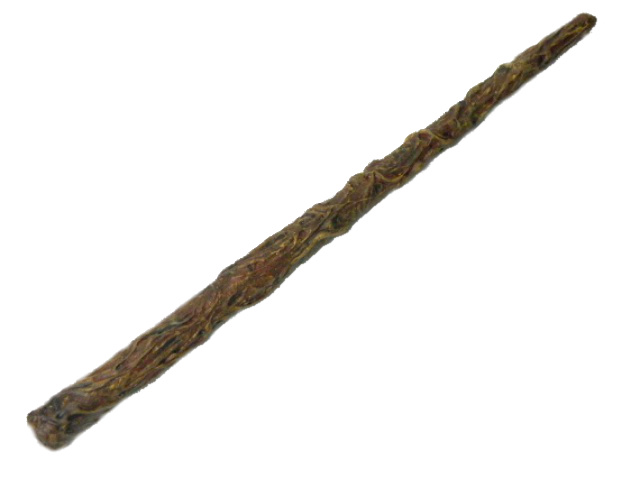
\includegraphics[width=.48\linewidth]{images/Gameplay/batonBoisSimple.jpg}}
	\hspace*{.04\linewidth}
	\subfloat[\label{subfig:batonBoisRune}Bâton de bois avec des runes décoratives et deux totems]{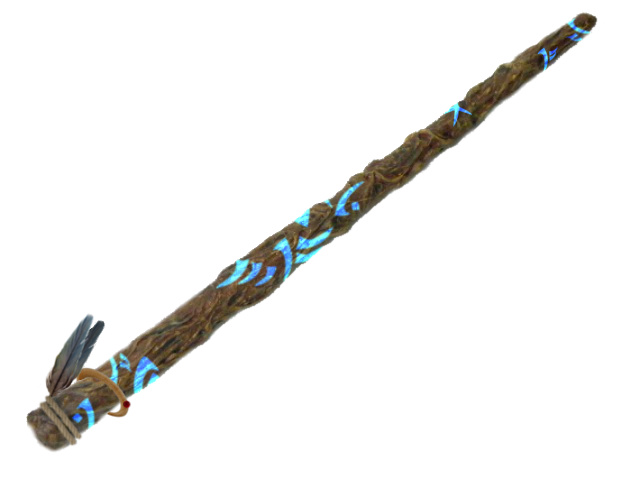
\includegraphics[width=.48\linewidth]{images/Gameplay/batonBoisRune.jpg}}
	
	\caption{Esquisse du bâton de bois {\cite{Baguettemagique_}}\label{fig:batonBois}}
\end{figureWithNotes}

\subsection{Sarbacane}
La sarbacane est un objet qui permet de tirer au loin de petites fléchettes. Cela ajoute une nouvelle distance, plus éloignée, au gameplay. Les fléchettes et leur éventuel contenu doivent être créés par le joueur. Il doit ainsi trouver le bois nécessaire aux dards (disponible en grande quantité, là ne réside pas le problème) mais surtout les recettes et ingrédients pour fabriquer les poisons à insérer dans les projectiles. À ce moment, le joueur peut créer des mixtures mortelles, soporifiques, empoisonnées, etc. L'idée derrière cet objet, le deuxième plus important du jeu, est de permettre au joueur de choisir entre une résolution de conflit \enquote{pacifique} ou meurtrière.

Pour le joueur, les recettes de poison sont de nouvelles récompenses et les ingrédients, éparpillés dans l'univers, devront être collectionnés (\anglicisme{item collecting}) afin de pouvoir finalement réaliser la potion désirée.




\chapter[Scénario et level design]{Scénario\\et level design}

\printMiniToc


\normalInfo{Level design}{Le \anglicisme{level design} est l'art de créer des niveaux bien équilibrés, fun à jouer et variés. C'est l'art de bien disposer les obstacles, récompenses et bâtiments pour que la difficulté soit adaptée. La carte doit présenter suffisamment de challenges pour motiver les joueurs, sans être excessivement difficile ce qui les empêcherait d'avoir une bonne expérience du jeu.}

\warningInfo{Niveaux déjà préparés}{Seul le premier acte du jeu est défini de manière détaillée. Le reste du jeu est brièvement décrit à la fin de ce chapitre.}

\section{Premier acte}
\label{sec:premierActe}

\subsection[Niveau 1 --- Course-poursuite avec la garde]{Premier niveau --- Course-poursuite avec la garde}
\label{sec:coursepoursuiteGarde}
\warningInfo{Un niveau d'importance}{Le premier niveau est crucial, c'est à la fois la scène d'exposition, l'opportunité de découvrir l'univers du jeu et l'apprentissage nécessaire des contrôles. S'il est bien réussi et fluide, le joueur pourra prendre plaisir à jouer et s'attacher à son personnage.}

Dans le premier niveau d'\nomJeu\ qui se déroule dans Redel, le joueur incarne Kida, l'héroïne. Elle est accompagnée par Lenaï, sa grande s\oe ur. Les premiers instants servent à l'apprentissage des commandes: se déplacer, courir, s'accroupir, sauter, etc. C'est la prise en main.

Puis vient l'élément déclencheur: deux gardes qui passent par l'avenue marchande, oublient négligemment un petit coffre au bord de l'étalage où ils viennent d'acheter de quoi manger. Kida ne peut s'empêcher de s'approcher pour observer la boîte mystérieuse. Tentée, elle la saisit sans avoir vraiment l'intention de la rendre. Mais au moment de commettre son délit, les gardes, ayant noté leur inadvertance, se retournent. À la vue des deux s\oe urs, ils leur hurlent d'arrêter; ces dernières prennent leurs jambes à leur cou et une course-poursuite s'engage.

Pour réussir le niveau, le joueur doit passer à temps les obstacles qui lui sont présentés afin de pouvoir s'enfuir. Ces empêchements ne doivent présenter qu'une faible difficulté pour permettre au joueur à la fois de s'habituer aux commandes et d'avoir une première impression aussi bonne que possible du jeu.

À la fin du niveau, Kida réussit à s'enfuir avec le coffre mais Lenaï est capturée et emmenée par la garde. Cet élément sera la cause des multiples péripéties qui s'ensuivront.

\normalInfo{Niveau de type \anglicisme{alley}}{Ce niveau est dit de type \anglicisme{alley}: à savoir, le joueur n'est pas libre de se balader selon sa propre volonté. À l'inverse, pour réussir le niveau, il doit suivre avec succès un chemin prédéfini.}

\subsection[Niveau 2 --- À la recherche de Lenaï]{Deuxième niveau --- À la recherche de Lenaï}
\label{sec:rechercheLenai}
\warningInfo{Objets à débloquer dans ce niveau}{\begin{itemize}
		\item Bâton de bois
		\item Trois sorts majeurs
		\item Tyrolienne
		\item Sarbacane
		\item Une recette de poison
	\end{itemize}
Si le nombre d'objets à débloquer est aussi important dans ce niveau, c'est que cela permet de lancer immédiatement le joueur au c\oe ur de l'action; dès le début du jeu, il possède des moyens pour interagir avec le monde virtuel qui l'entoure.
}

Le deuxième niveau débute le jour suivant. Kida part à la recherche de sa s\oe ur. Cette quête va cependant être entravée par le fait que la garde a bouclé les sorties du quartier pour retrouver le coffre volé; tout le monde est fouillé. Ainsi, l'héroïne se retrouve bloquée dans Redel. Faute de mieux, elle cherche à ouvrir le coffre volé, qui semble avoir nettement plus de valeur que ce qui aurait pu être supposé dans un premier temps.

La première tâche du joueur sera d'ouvrir le coffre. Il devra pour cela s'introduire par les toits dans la boutique du serrurier absent et utiliser ses machines pour créer une clé adaptée (puzzle\definition). Lorsque le coffre s'ouvre, un étrange animal en bondit. C'est la première rencontre avec un esprit de la Nature: Tia, l'écureuil vif et sauvage. La créature dit à Kida d'aller voir Maïnin, le vieux sage, puis s'enfuit en courant.

Le vieil homme, qui est en fait le gardien de l'accès au sanctuaire, y introduit la jeune fille (puzzle\definition\ pour activer le passage). Kida y rencontre Tia, qui lui explique les bases du fonctionnement de l'énergie verte, lui confie les trois premiers totems et le bâton de bois (voir les sections sur le \nameref{chap:gameplay}). L'esprit lui parle également d'un passage secret au c\oe ur du quartier naturel. Il donne accès à la rivière, puis à la tour de Gaamon dans laquelle Lenaï est sûrement enfermée.

Pour accéder à ce nouveau quartier, il faut résoudre toute une série de quêtes et de sous-quêtes pour finalement débloquer le passage indiqué par un \enquote{?} sur la maison mitoyenne de celle du cordonnier.

Au court du début de ce niveau, le joueur doit tirer profit des chemins sur les toits pour accéder aux endroits difficiles, pénétrer dans les maisons fermées et avancer dans l'histoire. Une carte des toits de Redel est donnée à la figure \ref{fig:carteQuartierPauvre}. Cet élément du Gameplay ajoute une dimension supplémentaire au jeu; le joueur doit utiliser le \enquote{z-axis} (que l'on pourrait traduire en français par la dimension verticale). Les passages par les toits ajoutent de plus un côté fun au jeu de même que les tyroliennes sur les rues, les passages secrets et les récompenses à débloquer par le joueur. Ils permettent de diversifier la façon de jouer.

Une fois le passage ouvert, un nouveau lieu est débloqué: le quartier naturel caché de Redel. Le joueur se voit alors confier par les Naturels une sarbacane, quelques dards et une première recette de poison. Si le joueur a déjà collectionné suffisamment d'ingrédients, il peut confectionner des dards supplémentaires. Les habitants du quartier ouvrent ensuite le passage situé sous la statue de Gaamon, au milieu de la place. L'héroïne peut ainsi accéder à la rivière et par extension, à la Tour.

\normalInfo{Niveau de type \anglicisme{island}}{Ce niveau, à l'inverse du précédent, représente un niveau de type \anglicisme{island}. Cela signifie que le joueur est libre de ses mouvements et peut aller où bon lui semble. Un autre terme pour décrire ce type de niveau serait semi open-world\definition.}

\begin{figure}[ph!]
	\centering	
	\subfloat[Plan du quartier pauvre]{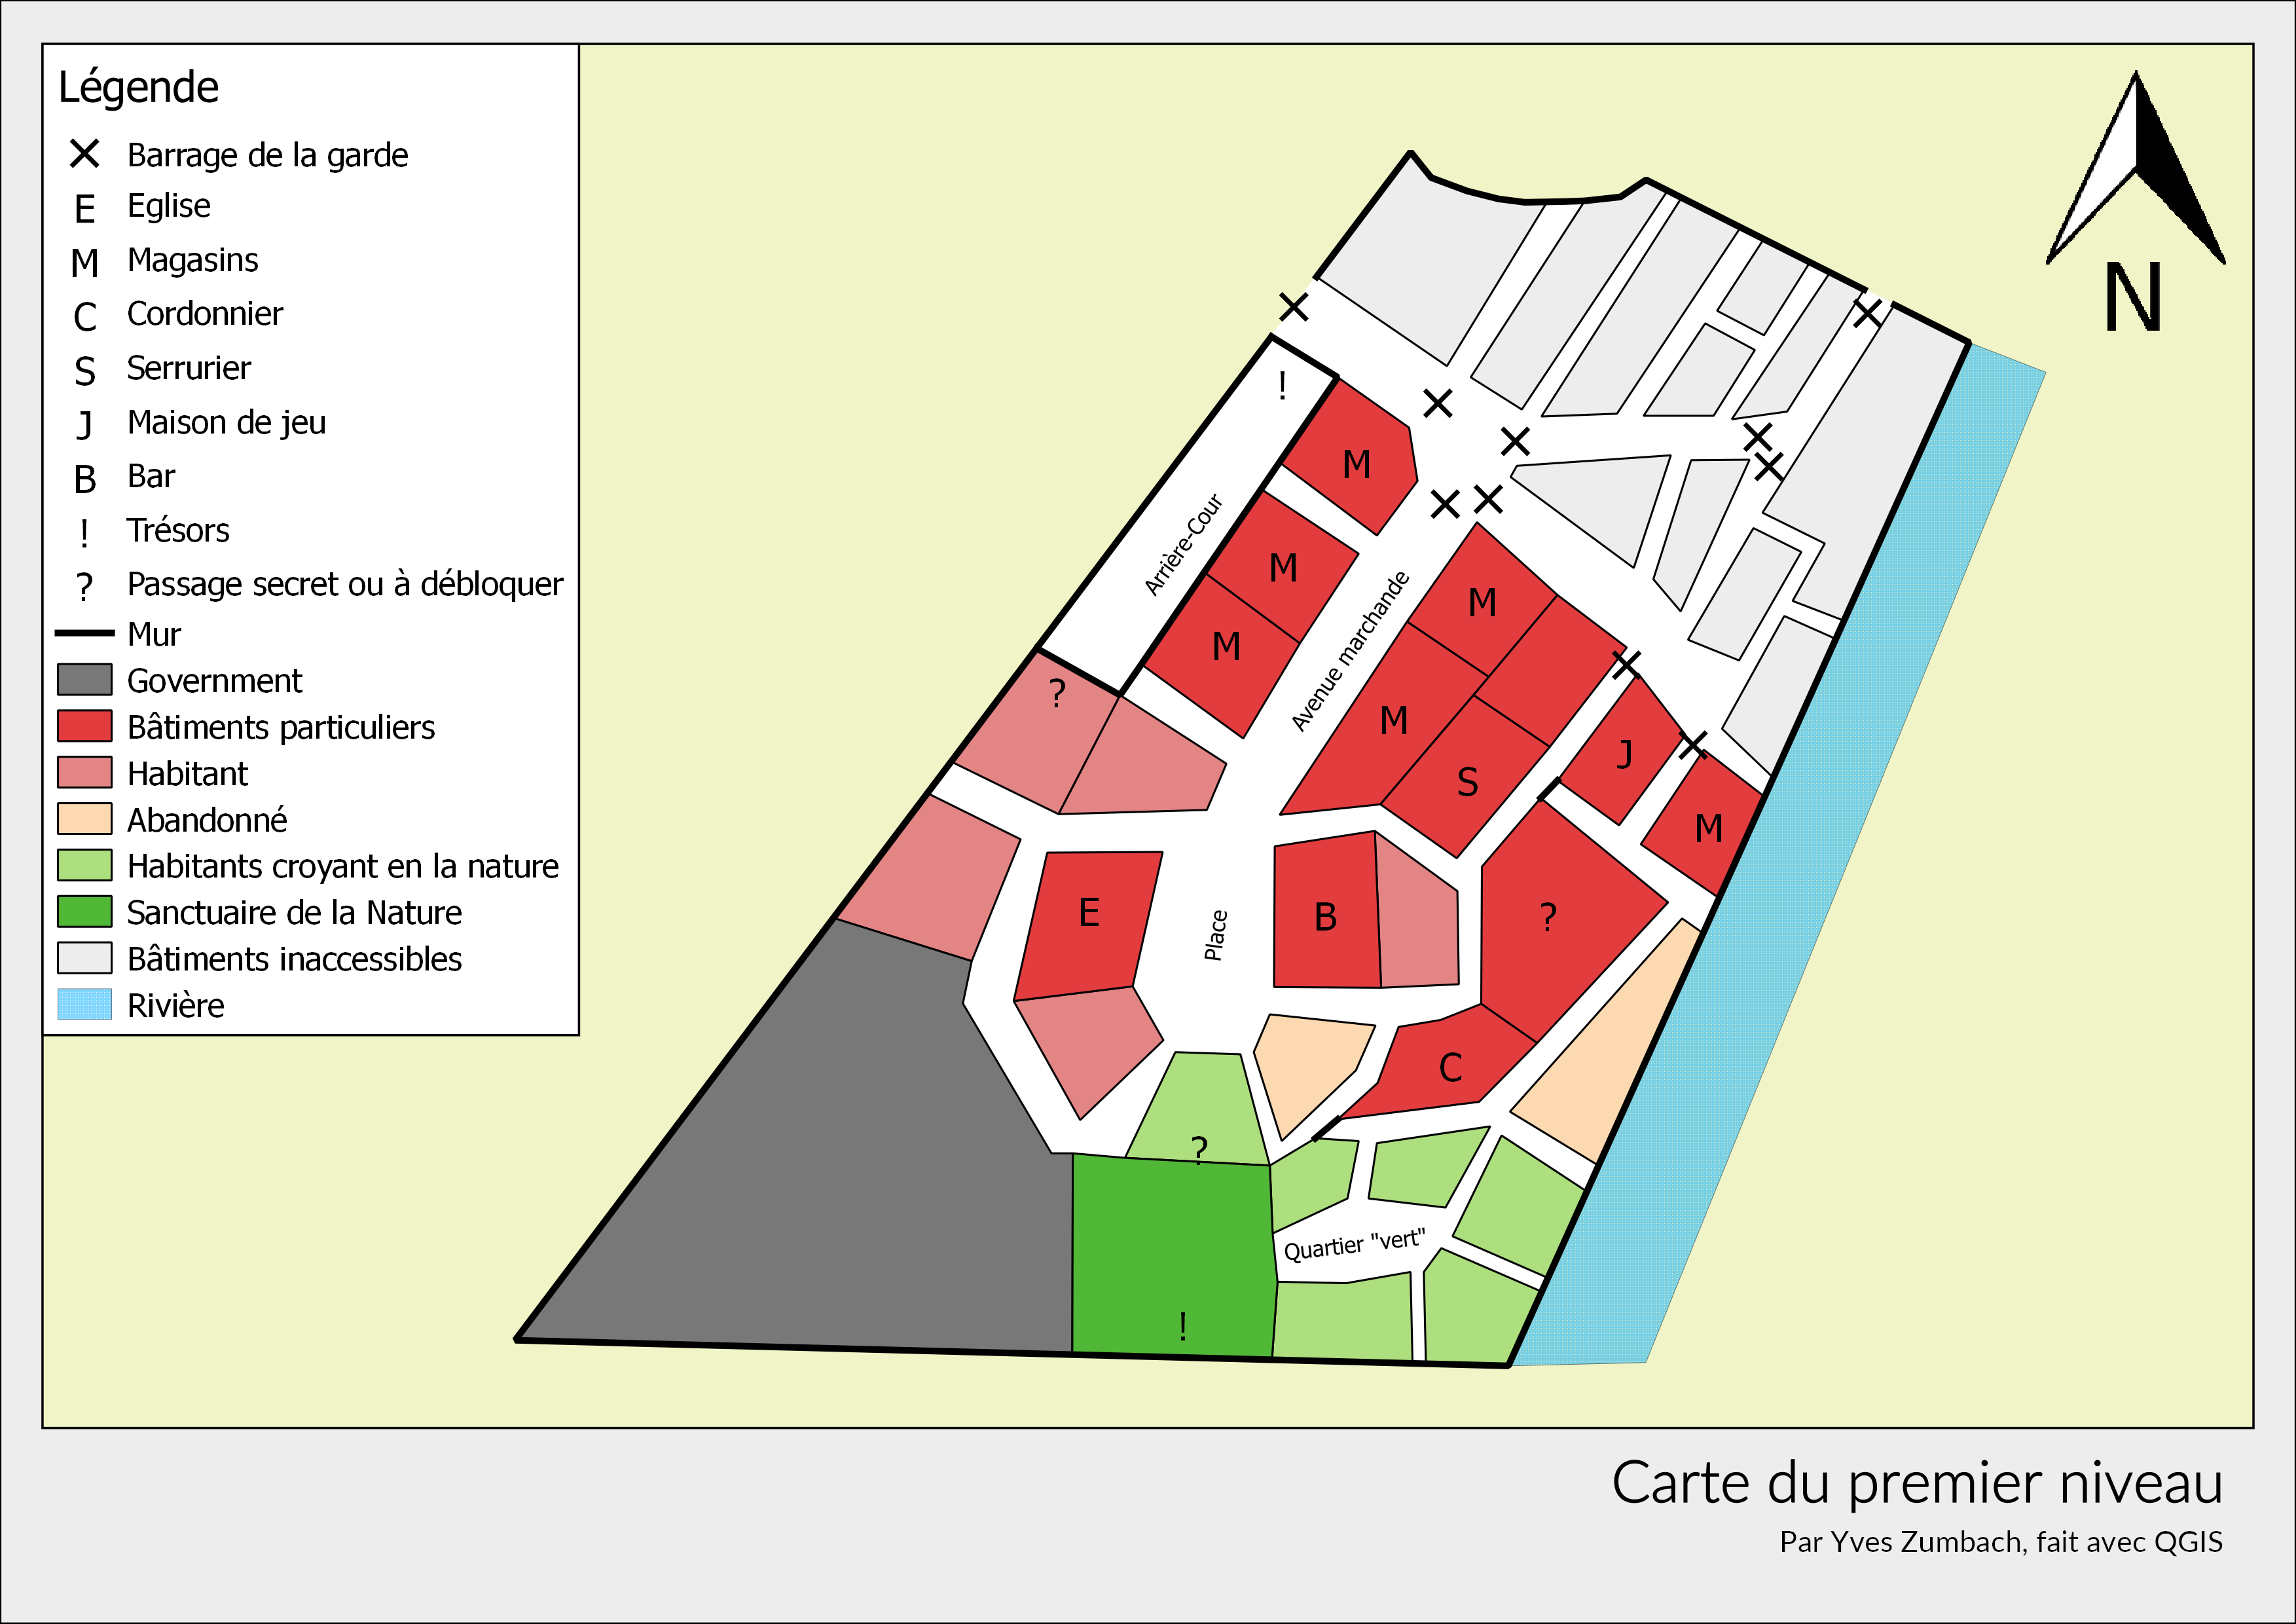
\includegraphics[width=\textwidth]{images/LevelDesign/cartePremierNiveauIndicationsGameplay.png}}
	
	\subfloat[Plan des toits]{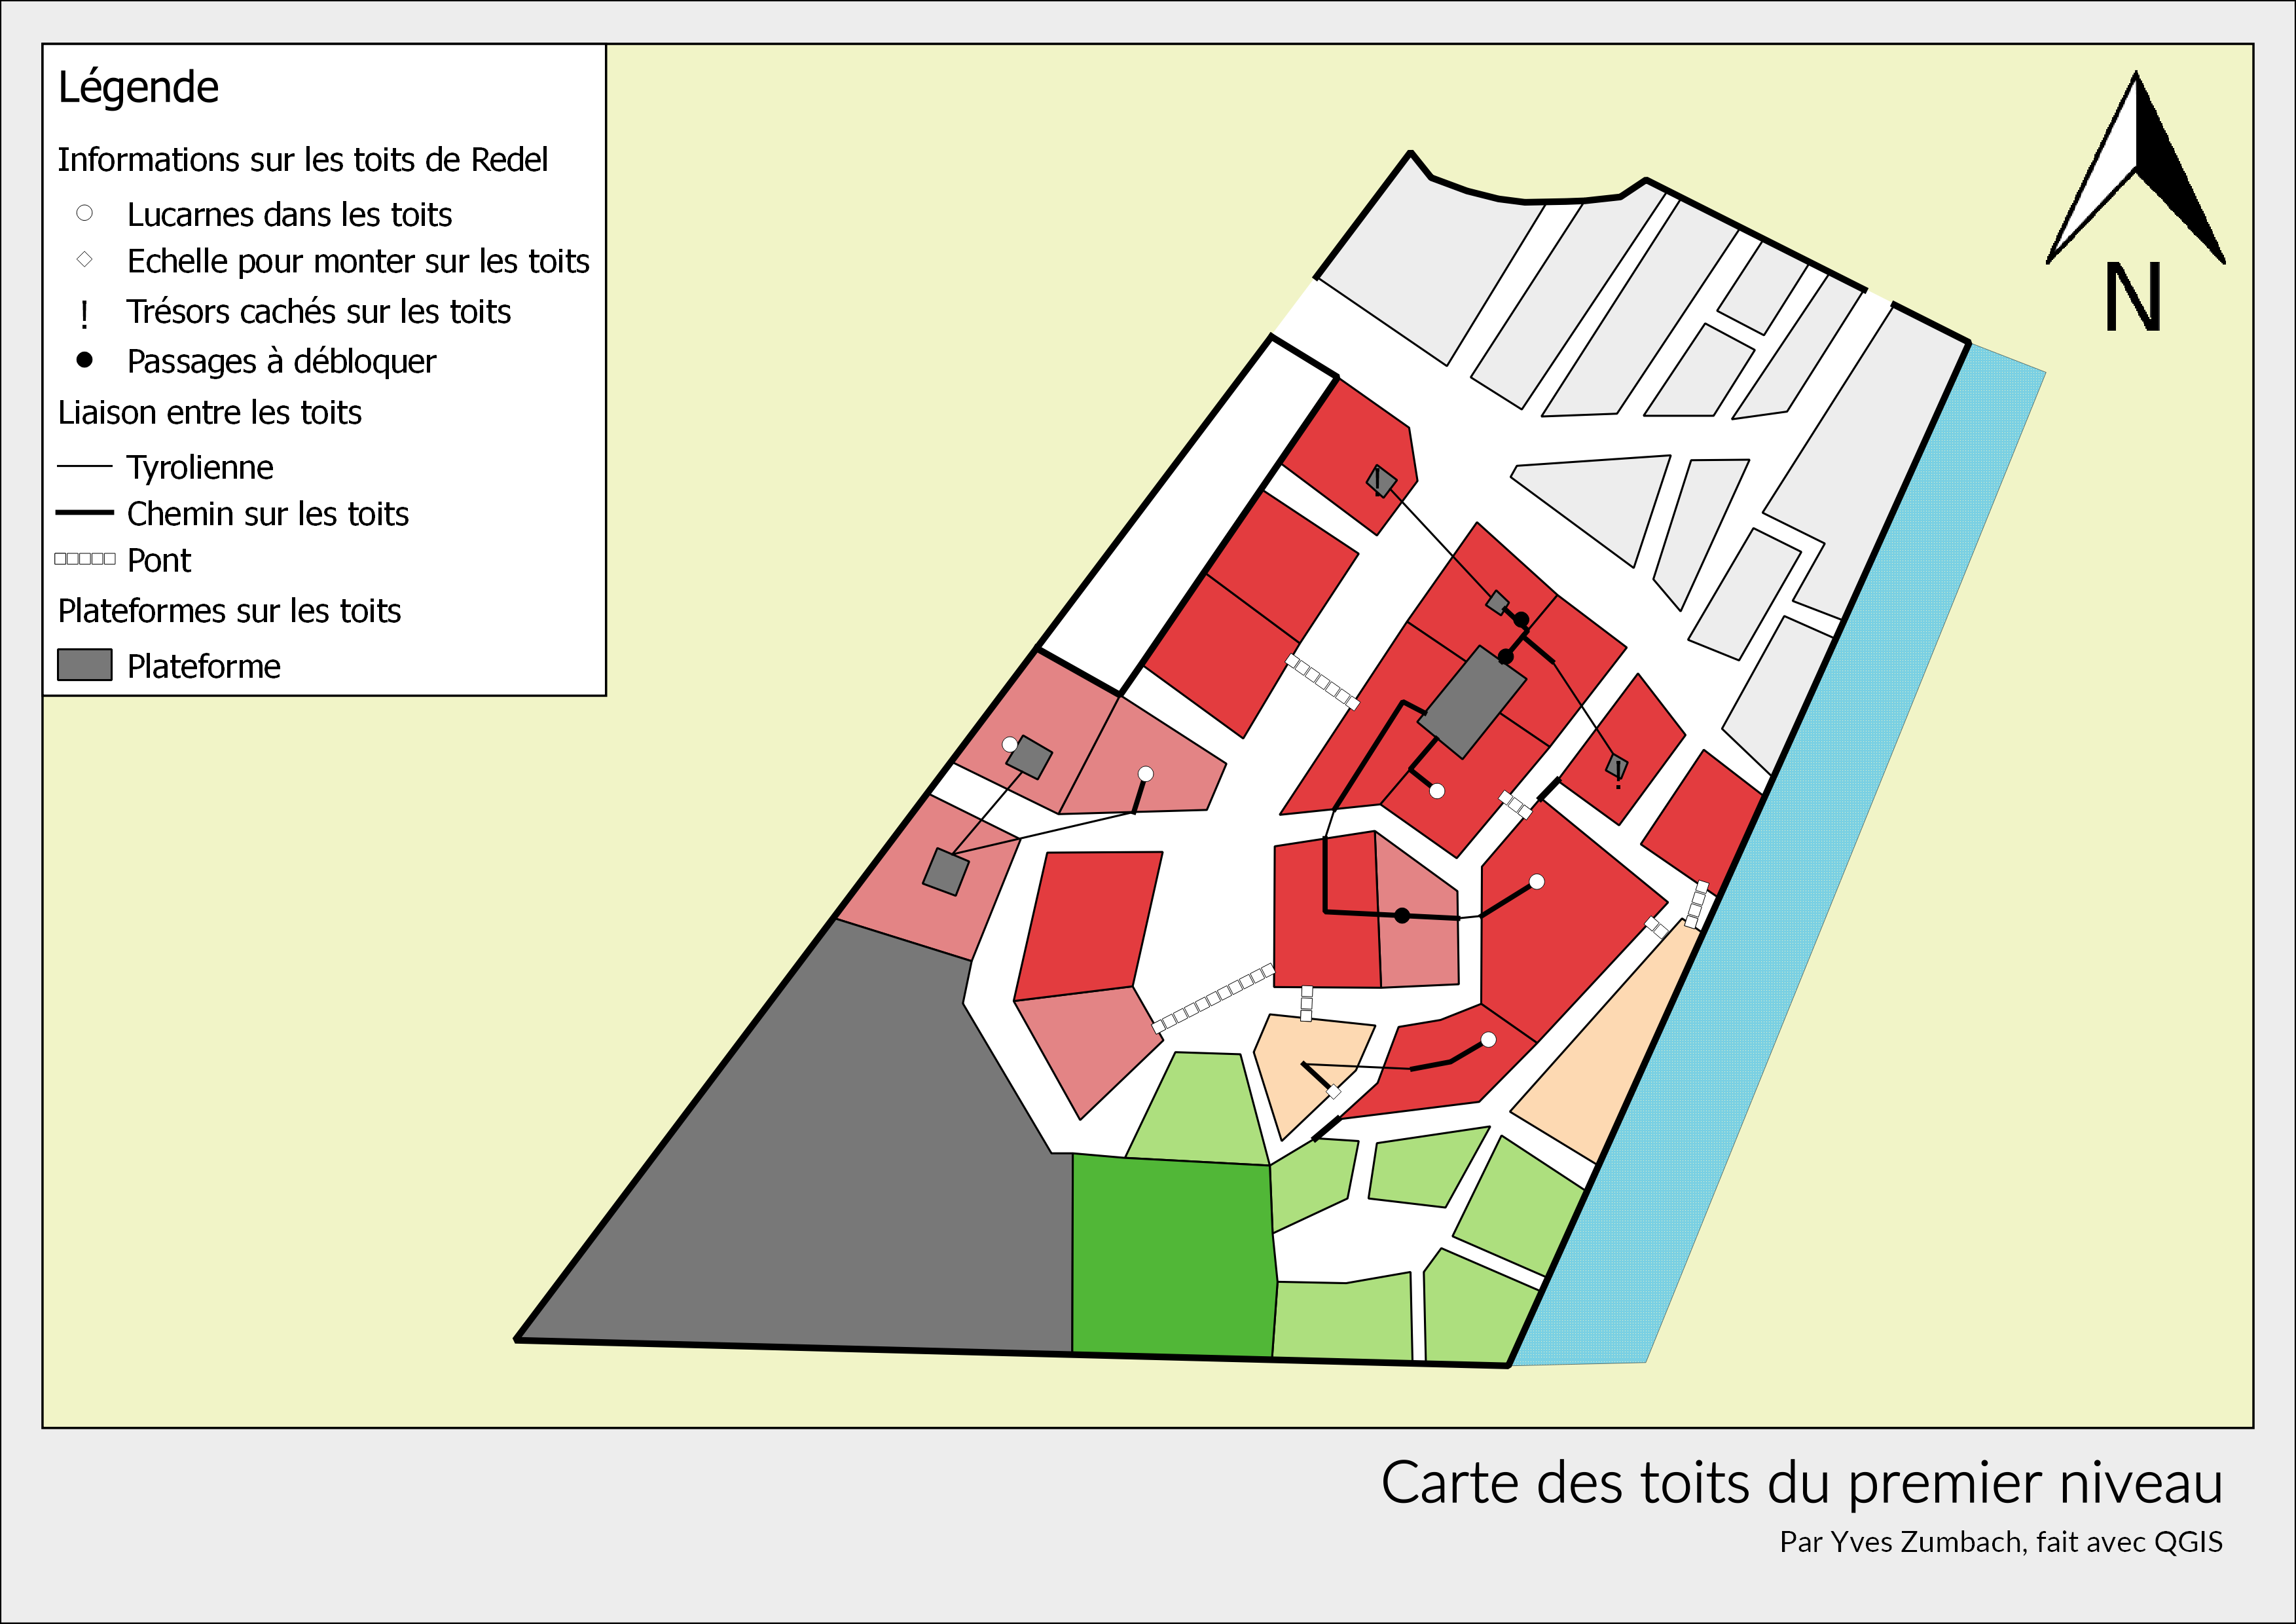
\includegraphics[width=\textwidth]{images/LevelDesign/carteToitsPremierNiveau.png}}
	
	\caption{\label{fig:carteQuartierPauvre}Cartes de Redel (réalisé à l'aide du programme Quantum GIS)}
\end{figure}


\subsection[Niveau 3 --- Dans l'antre du démon]{Troisième niveau --- Dans l'antre du démon}
\label{sec:entreDemon}
Kida pénètre dans le château de Gaamon par les souterrains. Ce niveau est un temple\definition. Il s'agira de trouver les cachots où Lenaï pourrait être enfermée. Le joueur le fera en résolvant des puzzles\definition\ pour accéder aux pièces suivantes (portes bloquées ou fermées) et éviter les ennemis (se référer à la partie \enquote{\nameref{chap:gameplay}} pour plus de détails).

Les objectifs intermédiaires du niveau seront de trouver la carte de la Tour, collecter des objets et des clés afin de pouvoir ouvrir les portes vers les salles suivantes.

Finalement, en arrivant aux cachots, Kida ne trouvera que des cellules vides... Aucune trace de Lenaï. C'est à ce moment que le boss\definition\ apparaît sous la forme d'une grande femme en armure. Le combat s'engage immédiatement. Kida se défend du mieux qu'elle peut, mais elle ne peut résister face à son adversaire parfaitement équipé pour le combat, aux armes aiguisées et techniques évoluées. Le joueur devra cependant survivre un certain temps au combat pour pouvoir avancer dans l'histoire. Il finit par se faire renverser et atterrit durement sur le sol, désarmé (cet élément pourrait être narré avec une cinématique). L'antagoniste lève son arme afin de porter le coup de grâce. Mais l'espace d'un instant, un éclair de doute traverse les yeux de la guerrière. Au même instant, Kida reconnait sa grande s\oe ur sous le masque terrifiant qu'elle porte: c'est contre Lenaï qu'elle s'est battue! L'hésitation à porter le coup fatal suffit à Kida qui profite de l'ouverture pour s'échapper, se précipiter vers la fenêtre la plus proche et sauter droit dans les douves... à l'extérieur de la ville.

\criticalInfoDarkRed{Importance du troisième niveau}{Le troisième niveau est véritablement la clé de voûte de l'histoire. On y découvre que Lenaï est passée du côté de Gaamon. Cet élément capital sera la cause des multiples péripéties de l'histoire d'\nomJeu.

Ce retournement étrange s'explique par le fait que Gaamon, le père de Lenaï, accueille, à son arrivée dans la Tour, sa fille disparue comme jamais la jeune femme n'avait été traitée. Il demande à la garde de la libérer de ses liens et l'emmène au c\oe ur de la Tour. Là, il se comporte comme le père qui a toujours manqué à Lenaï. Il lui apporte l'attention, l'affection et l'amour dont elle avait toujours rêvé, et qui lui faisait cruellement défaut depuis la mort de leur mère. Lenaï se réfugie dans ce havre de paix et de bonheur que son père crée autour d'elle. C'est pour défendre cette relation, qu'elle accepte de commettre certains actes parmi les plus répréhensibles. Son père l'aime et la protège mais, implicitement, elle sait que pour conserver son amour, il lui faut accepter de devenir celle que Gaamon veut qu'elle soit: son bras armé, la générale de ses troupes. Le revirement est donc brutal et Lenaï commet de nombreux crimes afin de conserver sa situation.
}

\section{Jouer Lenaï}
La plupart des niveaux sont joués avec Kida. Cependant, certains utiliseront Lenaï comme personnage. Cela apporte un énorme avantage technique: la réutilisation des niveaux et contenus déjà réalisés. En même temps, cette façon de faire offre des points de vue diversifiés à l'histoire, ce qui la rend plus intéressante. Mieux encore, cela permet au joueur d'avoir un aperçu de la vie de Lenaï. C'est ce dernier point qui a le plus de valeur pour moi. Il permet d'approfondir le personnage de Lenaï, de Gaamon et le gameplay: lorsqu'on joue Lenaï, on est forcé d'exécuter les ordres de Gaamon, il faut donc compléter les missions données par le grand ennemi du jeu.

C'est premièrement une façon de découvrir Gaamon, ainsi que sa base. Cela permet au joueur d'obtenir un aperçu des forces ennemies, et de fonctionner comme un espion dans l'antre ennemi. Ces niveaux seront aussi l'occasion d'explorer la relation entre Lenaï et Gaamon, à la fois paternelle et ambivalente car Lenaï, bien qu'elle soit \enquote{ensorcelée}, perçoit bien que ce qu'elle fait est immoral et injuste.

Enfin, le tyran commandant à ses subordonnés des missions à l'éthique hautement critiquable comme collecter des impôts énormes chez les paysans autour de la ville, aller éradiquer la Nature sur une surface toujours grandissante autour de la cité, etc, ces missions seront l'occasion de proposer un choix au joueur quant à leur résolution. Par exemple pour la collecte des impôts, le joueur pourra mettre à sac les maisons des habitants incapables de payer pour trouver jusqu'à la dernière pièce, une solution simple et efficace, ou alors faire l'effort de  trouver lui-même des pièces (la possibilité lui en sera donné) pour aider les personnes les plus en difficulté.



\section{Deuxième acte}
\label{sec:deuxiemeActe}
Kida se retrouve hors des murs pour la première fois de sa vie. Elle doit s'habituer à un nouveau mode de vie plus rural, plus sauvage et découvrir les populations environnant \nomVille. Ces personnes sont pour la plupart des renégats ou des paysans ayant fui lors de la création de la ville. La vie est très dure. Gaamon, s'il tolère ces personnes, ne les épargne pas pour autant. Elles se font voler par la garde, les impôts prélevés sont ridiculement élevés, parfois même, Gaamon envoie ses machines détruire une ou deux maisons afin de tester leur efficacité. Ces gens ont donc appris à se cacher et savent détecter l'arrivée des soldats. Beaucoup parmi eux seraient même près à se battre mais la supériorité militaire de Gaamon est indubitablement écrasante. Ils se tiennent prêts au combat mais attendent l'occasion opportune et survivent en attendant.

Kida y apprend la légende fantastique du peuple des \nomNaturels s, un peuple technologiquement extrêmement avancé, beau, raffiné et puissant. C'est ce mythe qui fait espérer encore les exclus; pour eux, il existe encore une chance. C'est ce mythe aussi qui va décider Kida. Pour sauver sa s\oe ur, elle se met à la recherche de ce peuple fantastique, convaincue que si elle arrive à bâtir un monde meilleur avec l'aide de ces gens, son aînée verra l'absurdité de ses actions et qu'elle la rejoindra.

Piste après piste, bribe après bribe d'information, son chemin la conduira finalement à découvrir, caché au fond d'une forêt sombre et majestueuse, un très ancien temple à l'architecture gracieusement étrange, sortie tout droit d'un autre âge: un temple teluran. C'est en haut de ce dernier qu'elle trouve un engin volant qui, une fois réveillé, la conduit automatiquement sur les hauts-plateaux, où le peuple persécuté a trouvé refuge. Kida vient de trouver un des derniers moyens de retrouver les Telurans que ces personnes éclairées avaient laissé aux Hommes.

\section{Troisième acte}
\label{sec:troisiemeActe}
Une fois arrivée chez les Telurans, Kida découvre que le peuple magnifique en lequel elle espérait n'est plus que l'ombre de lui-même. Les persécutions incessantes de Gaamon ont fini d'achever les dernières merveilles de ce peuple: le palais royal tombe en ruine, l'art qui en faisait jadis la gloire est maintenant tombé en ruine, oublié, mais surtout, les secrets de l'énergie verte sont tous perdus. La vie est devenue dure. Sans sa source vitale, la glorieuse nation survit à peine; tous les habitants travaillent aux champs ou dans les ateliers et la connaissance, la science, la notion de beau, d'élégant, l'essence même du peuple se perdent inexorablement.

Profondément choquée par cet état pitoyable, que les Telurans ne peuvent rien pour sa s\oe ur, Kida part à la recherche des secrets de l'énergie verte. Après de longues recherches, elle rencontre finalement l'esprit de la Nature Léo dans la forêt de Tylor. Les esprits ne prennent normalement pas part aux affaires du monde et se contentent d'être spectateur des époques et des peuples naissants, arrivant à leur apogée puis déclinants. Cependant, confronté au récit qui lui est fait, Léo, esprit impulsif, décide d'enseigner à Kida les secrets de la grande salle.

Cette connaissance retrouvée et la grande salle remise en marche, la cité telurane retrouve d'elle-même sa gloire passée, les bâtiments renaissent, les animaux reviennent parmi le peuple, l'art et la musique redeviennent ce qu'ils auraient toujours dû être et s'élèvent d'eux-mêmes, la beauté de la vie se mêle à nouveau au chant de la Nature.

\section{Quatrième acte}
\label{sec:quatriemeActe}
À ce point du jeu, le joueur a déjà joué plusieurs niveaux dans la peau de Lenaï. Un ultime niveau de ce type permet de mettre en évidence l'impact que les horreurs de Gaamon ont sur Lenaï. Elles la poussent à se révolter contre l'image paternelle et elle fuit la cité humaine à bord d'un dirigeable blindé vers les hauts-plateaux où elle retrouve les Telurans et Kida. Cette dernière apprend ainsi l'identité de son géniteur, elle n'est autre que la fille de son pire ennemi. Et si tout le monde se montre méfiant d'abord à l'égard de Lenaï, les informations alarmantes qu'elle apporte dissipent rapidement les soupçons: Gaamon a atteint la phase finale de son plan; il a prévu la destruction totale de toute Nature... et des Telurans. 

Il a constitué une immense armée de machines, amassées devant les murailles de Murtos, qu'il s'apprête à lancer sur toutes les forêts d'Éluria. Kida, aidée de sa s\oe ur, doit donc retrouver les derniers secrets manquants de l'énergie verte afin de donner aux Telurans suffisamment de puissance pour affronter et démanteler les troupes mécaniques. Et ce sont les mystères des machines volantes teluranes qu'il faut retrouver pour accomplir un tel miracle.

On peut ensuite imaginer un immense combat aérien entre les machines volantes et légères des Telurans et les dirigeables blindés des factions humaines. Les humains prenant l'avantage, Kida comprend que le seul moyen de remporter la victoire est de tuer son père. Kida et Lenaï, côte-à-côte à bord d'un aéronef propulsé à l'énergie verte, se jettent alors sur la tour de verre depuis laquelle leur père contrôle ses forces. Le combat final entre Gaamon, utilisant toutes ses machines, et les deux s\oe urs dévoile le dernier secret du monstre: il a remplacé la plupart des parties de son corps par des membres robotisés. Finalement le tyran est défait. Son armée tombe alors immédiatement en pièce: Gaamon était la clé qui maintenait l'univers des Hommes debout.

Kida et Lenaï pénètrent dans le c\oe ur sacro-saint de la Tour, la seule pièce que Gaamon avait toujours interdite à Lenaï. Elles y découvrent une salle aux couleurs chatoyantes; un magnifique portrait de Miya est accroché glorieusement au milieu du mur faisant face à la porte d'entrée. Sous ce dernier sont couchées de fraîches et belles fleurs orange. L'histoire se termine avec la découverte d'un vieux livre, sous les fleurs, narrant le conte tant affectionné de Miya et Gaamon dont ils ont tiré le nom de leur première fille Lenaï.



%\chapter{Musique maestro!}
%\printMiniToc

Sans la musique, la vie serait une erreur.
Friedrich Nietzsche

\section{La musique dans les jeux vidéos}
La bande son d'un jeu vidéo est un élément tellement important qu'elle permet à elle seule de reconnaître certains jeux. Tous ceux qui auront joué à \textit{The Legend of Zelda: The Minish Cap} reconnaîtront le thème des champs d'Hyrule, par exemple. Elle est la clé de voute d'une ambiance réussie et permet de changer le ton d'une scène à elle seule.

\section{Deux types de sons dans un jeu vidéo}
Les jeux vidéos son composés de deux types de sons: le thème et les effets sonores. Le premier désigne la musique de fond qui déterminera l'ambiance globale. Les effets sonores, quant à eux, sont tous les petits bruits qui sont déclenchés par les actions dans le jeu: ouverture d'une porte, déclenchement d'une attaque, pas sur le sol, etc. À chacun correspond un type de fichier différent et une gestion spécifique.

Inclure du son dans le pdf?

\chapter{Réalisation technique}

\printMiniToc

%\textit{Ce chapitre se concentre sur différents aspects de la réalisation technique: outils utilisés, techniques bien pratiques dans l'univers des jeux vidéo, etc. Je décris ici aussi les problèmes techniques les plus importants que j'ai rencontré.}

\section[Workflow]{\anglicisme{Workflow}*}
La création d'un jeu passe par deux étapes principales:
\begin{itemize}
	\item La modélisation des objets présents dans le jeu.
	\item Leur intégration dans un moteur de jeu\definition\ au moyen d'un langage informatique.
\end{itemize}
\vspace{\baselineskip}

\begin{figure}[ht!]
	\begin{center}
		\begin{tikzpicture}
			\node[auto, rectangle, thick, draw = black, text width=2.5cm, text centered, minimum height=4em, rounded corners=2pt] (modelisation) {Modélisation des contenus};
			\node[right of=modelisation, thick, draw=black, node distance = 4.5cm, auto, rectangle, text width=3.1cm, text centered, minimum height=4em, rounded corners=2pt] (moteur) {Intégration dans un moteur de jeu};
			\node[right of=moteur, thick, draw=black, node distance = 4cm, auto, rectangle, text width=1.7cm, text centered, minimum height=4em, rounded corners=2pt] (jeu) {Jeu vidéo\\};
			
			\path [ultra thick, draw, -latex', >=latex] (modelisation) -- (moteur);
			\path [ultra thick, draw, -latex', >=latex] (moteur) -- (jeu);
			
			\node [fit=(modelisation) (moteur)] (fit) {}; 
			\node [fit=(jeu)] (fit2) {};
			\draw [decorate, decoration={brace,amplitude=10pt, mirror},line width=1pt] (fit.south west) -- (fit.south east) node [black,midway,yshift=-0.6cm]  {Processus};
			\draw [decorate, decoration={brace,amplitude=10pt, mirror},line width=1pt] (fit2.south west) -- (fit2.south east) node [black,midway,yshift=-.6cm]  {Résultat};
			
			%\node [above right = of moteur, xshift=-2mm, yshift=-3mm] (dashedTop) {};
			%\node [below right = of moteur, xshift=-2mm] (dashedBottom) {};
			%\draw [dashed, thick] (dashedTop) -- (dashedBottom);
		\end{tikzpicture}
	\caption{Workflow de la création d'un jeu vidéo}
	\end{center}
\end{figure}

Un objet désigne n'importe quel élément visible. C'est ainsi une entité qui possède une géométrie; cela inclut, par exemple, les bâtiments, les meubles, la nourriture ou encore les véhicules. Tous les contenus d'un jeu vidéo, qu'ils soient en 2 ou 3 dimensions, doivent être créés de façon informatique. Dans le cas d'un jeu à 2 dimensions, des logiciels comme Gimp --- ou Photoshop, son équivalent propriétaire --- seraient utilisés pour créer des images qui seraient animées directement dans le moteur de jeu. L'ajout d'une nouvelle dimension complique cependant passablement le processus de création: il faut utiliser des programmes spécialisés, plus complexes, pour modéliser des objets dans l'espace. Les animations doivent, elles aussi, être créées dans ces programmes, car les fonctionnalités d'un moteur de jeu ne permettent en majorité pas de les réaliser. Seul le contrôle (et non pas la réalisation) des animations est effectué depuis le moteur de jeu.

Une fois créés, il est nécessaire de mettre tous les objets ensemble pour qu'ils forment un tout cohérent --- un niveau. Il faut programmer les actions du joueur, vérifier que le jeu suit bien le scénario, gérer le son et travailler sur l'ambiance du jeu. Tout cela est réalisé dans le moteur de jeu par programmation.


\subsection[Workflow des programmes]{\anglicisme{Workflow} des programmes}
La figure \ref{fig:workflowProgrammes} illustre le \anglicisme{Workflow} des programmes principaux utilisés dans le cadre de ce Travail de Maturité. %De plus amples détails sur les programmes sont donnés à la section \ref{sec:programmes}.

\begin{figure}[ht!]
	\center
	\begin{tikzpicture}	
		\node[node distance=4.45cm, auto, rectangle, thick, draw = black, text width=2.5cm, text centered, minimum height=4em, rounded corners=2pt] (skp) {Sketchup};
		
		\node[above of=skp, node distance=2cm, auto, rectangle, thick, draw = black, text width=2.5cm, text centered, minimum height=4em, rounded corners=2pt] (gimp) {GIMP};
		
		\node[below of=skp, node distance=2cm, auto, rectangle, thick, draw = black, text width=2.5cm, text centered, minimum height=4em, rounded corners=2pt] (mh) {MakeHuman};
		
		\node[right of=skp, node distance=5cm, auto, rectangle, thick, draw = black, text width=2.5cm, text centered, minimum height=4em, rounded corners=2pt] (blend) {Blender};
		
		\node[above of=blend, node distance=2cm] (aboveBlend) {};
		
		\node[below of=blend, node distance=2cm] (underBlender) {};
		
		\node[right of=blend, node distance=4.45cm, auto, rectangle, thick, draw = black, text width=2.5cm, text centered, minimum height=4em, rounded corners=2pt] (gd) {Godot};
		
		\node[below of=gd, node distance=2cm, auto, rectangle, thick, draw = black, text width=2.5cm, text centered, minimum height=4em, rounded corners=2pt] (auda) {Audacity\\(Son)};
		
		\path [ultra thick, draw, -latex', >=latex] (skp) -- (blend) node [midway, text width = 1.8cm] {Kerkythea \\ et jkt2obj};
		\path [ultra thick, draw, -latex', >=latex] (gimp) -- (blend);
		\path [ultra thick, draw, -latex', >=latex] (mh) -- (blend);
		\path [ultra thick, draw, -latex', >=latex] (auda) -- (gd);
		\path [ultra thick, draw, -latex', >=latex] (blend) -- (gd);
	\end{tikzpicture}
	\caption{Les programmes utilisés pour la réalisation de ce Travail de Maturité \label{fig:workflowProgrammes}}
\end{figure}


\section{Programmes}
\label{sec:programmes}
\subsection{Modélisation 3D}
\label{sec:modelisationContenu3D}
J'utilise Blender pour la modélisation des contenus 3D de mon jeu. C'est un programme gratuit, open source et soutenu par une grande communauté. Très complet, il rivalise avec les plus grands logiciels propriétaires. Il permet de créer des objets, de leur donner couleurs et textures (\textit{cf.} section \ref{sec:textures}), de les animer et bien plus encore. Initialement prévu pour faire des films d'animation, il est tout à fait recommandé de l'utiliser dans le cadre de la création de jeux vidéo.

\begin{center}

\includegraphics[width=.5\textwidth]{./images/Technique/blender-plain.png}
\\[-4mm]\hspace*{5mm}\url{www.blender.org}
\end{center}

Les films officiels de la Blender Foundation, disponibles sur Youtube, donnent un bon aperçu des capacités du programme: \textit{Elephant dream} (2006), \textit{Big Buck Bunny} (2008), \textit{Sintel} (2010) ou encore \textit{Tears of steel} (2013).

J'utilise également Google Sketchup. Ce programme de modélisation --- bien moins puissant et développé que Blender --- est cependant nettement plus simple à utiliser et possède l'avantage d'être lié à la 3D Warehouse de Google (littéralement \enquote{entrepôt 3D}): un site web recensant des milliers d'objets réalisés avec ce logiciel.

La réalisation des contenus d'un jeu vidéo est une étape très longue et demande des connaissances poussées de modélisation, design et programmation. C'est une tâche dont s'occupe en général une équipe complète. La réalisation de \textit{Grand Theft Auto V} a par exemple nécessité la collaboration de plus de 1000 personnes \cite{RockstarMorethan1000peoplemadeGTAV_}. Étant seul, je me servirai de la 3D Warehouse pour trouver la plupart des modèles que j'utiliserai, afin de tenter de finir une version de démonstration du jeu dans un temps raisonnable. Il est cependant à noter que, bien que la 3D Warehouse soit une ressource énorme, les contenus qu'elle propose ne correspondent pas toujours aux besoins du jeu. Il faut donc modifier la plupart de ces éléments afin qu'ils soient adaptés.


\subsubsection{Problème de format d'objet 3D}

\begin{figure}[ht!]
	\center
	\begin{tikzpicture}
	\node[auto, rectangle, thick, draw = black, text width=2.5cm, text centered, minimum height=4em, rounded corners=2pt] (skp) {.skp\\(Sketchup)};
	
%	\node[left of=skp, node distance= 2cm, auto, text width=2.5cm, text centered, minimum height=4em] (par1) {\Huge(};
	
	\node[right of=skp, node distance=3.7cm, auto, rectangle, thick, draw = black, text width=2.5cm, text centered, minimum height=4em, rounded corners=2pt] (xml) {.xml\\(Kerkythea)};
	
	\node[right of=xml, node distance=3.7cm, auto, rectangle, thick, draw = black, text width=2.5cm, text centered, minimum height=4em, rounded corners=2pt] (obj) {.obj\\(jkt2obj)};
	
%	\node[right of=obj, node distance= 2cm, auto, text width=2.5cm, text centered, minimum height=4em] (par2) {\Huge)};
	
	\node[below of=obj, node distance=2.5cm, auto, rectangle, thick, draw = black, text width=2.5cm, text centered, minimum height=4em, rounded corners=2pt] (blend) {.blend\\(Blender)};
	
	\node[left of=blend, node distance=3.7cm, auto, rectangle, thick, draw = black, text width=2.5cm, text centered, minimum height=4em, rounded corners=2pt] (dae) {.dae\\(Blender exporter)};
	
	\node[left of=dae, node distance=3.7cm, auto, rectangle, thick, draw = black, text width=2.5cm, text centered, minimum height=4em, rounded corners=2pt] (scn) {.scn\\(Godot)};
	
	\path [ultra thick, draw, -latex', >=latex] (skp) -- (xml);
	\path [ultra thick, draw, -latex', >=latex] (xml) -- (obj);
	\path [ultra thick, draw, -latex', >=latex] (obj) -- (blend);
	\path [ultra thick, draw, -latex', >=latex] (blend) -- (dae);
	\path [ultra thick, draw, -latex', >=latex] (dae) -- (scn);
	\end{tikzpicture}
	\caption{Les différents formats 3D utilisés durant ce TM \label{fig:formats3D}}
\end{figure}

Certains domaines de l'informatique existent depuis relativement longtemps et bénéficient à ce titre de normes bien établies. C'est le cas, par exemple, de la gestion/création/modification d'image. Les formats .png et .jpg sont connus de tous. Au même titre, la bureautique dispose d'outils matures comme Libre Office ou Word et les formats correspondants (.odt et .doc) sont maintenant supportés très largement.

Il n'en est pas de même pour l'univers de la 3\textsuperscript{e} dimension. Les logiciels implémentant de telles fonctionnalités ont chacun créé leur propre format; il n'existe malheureusement pas de consensus à ce niveau. L'utilisation conjointe de la 3D Warehouse, Blender et Godot a donc posé des problèmes de compatibilité.

La transition de la 3D Warehouse à Blender et finalement à Godot n'est de loin pas transparente et nécessite un certain nombre de manipulations. Les fichiers provenant d'internet sont donc ouverts avec Google Sketchup puis exportés avec un petit add-on nommé Kerkythea vers le format .xml. Ce dernier est ensuite converti grâce à jkt2obj en un fichier .obj que Blender peut importer, bien que ce ne soit pas son format natif. Le résultat de la conversion n'est jamais certain au vu de sa complexité. Il n'est d'ailleurs pas rare qu'à leur arrivée dans Blender, les objets possèdent des défauts: sommets dupliqués, faces mal connectées, problèmes de texture, etc.

C'est dans Blender que toutes les modifications sur les objets sont effectuées. Ces derniers sont ensuite exportés au format .dae (pour les scènes complètes) ou .obj (pour les objets sans animation) vers Godot qui les stocke finalement au format .scn. Un diagramme montrant ce \enquote{\anglicisme{Workflow} des formats 3D} est donné à la figure \ref{fig:formats3D}.



\subsubsection{Un ordre d'idée: modélisation d'une maison}

\begin{figure}[ht!]
	\center
	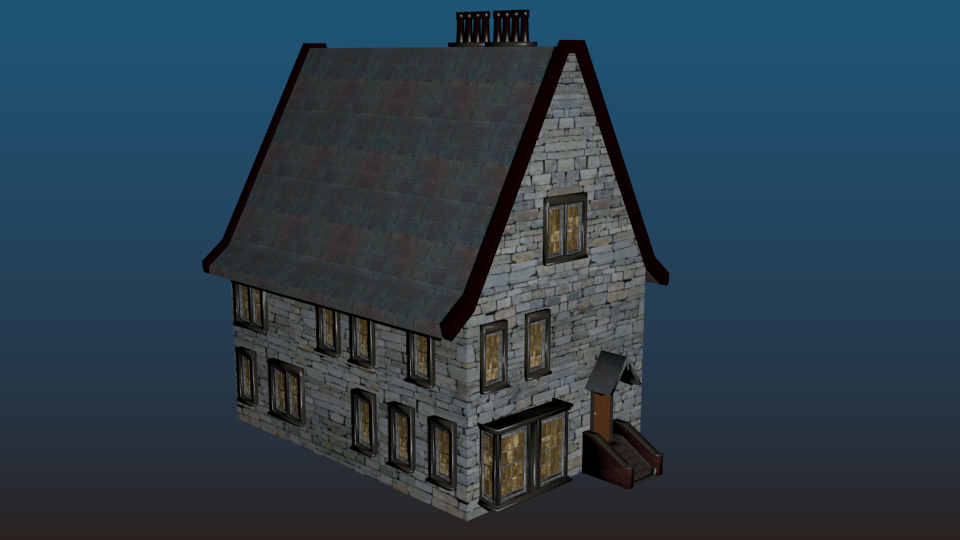
\includegraphics[width=\textwidth]{images/Technique/modelisationMaison.png}
	\caption{\label{fig:modelisationMaison}Une maison réalisée dans Blender}
\end{figure}

Voilà les éléments qui ont été nécessaires pour modéliser la maison qu'on peut voir à la figure \ref{fig:modelisationMaison}:
\begin{itemize}
	\item Le toit: Modélisé à la main; la texture qui permet de simuler les tuiles vient de la 3D Warehouse.
	\item La bordure du toit: Modélisée à la main; cet objet n'a pas de texture mais un seulement un matériau\footnote{Un matériau est un moyen de donner de la couleur à un objet. À l'inverse des textures qui sont des images souvent complexes, les matériaux sont des couleurs unies. On en configure certaines caractéristiques: réflexion, transparence, diffraction de la lumière, etc.} réalisé dans Blender.
	\item Mur de la maison: La géométrie a été réalisée à la main. La texture de mur en pierre provient d'Internet.
	\item La porte: Modélisée à la main, c'est en fait un amalgame de trois objets: le cadre de la porte, la porte et la poignée de la porte. Chacune des parties a son propre matériau.
	\item Les fenêtres simples (9x), doubles (3x) et doubles proéminentes, les cheminées (2x), l'avant-toit et les escaliers proviennent de la 3D Warehouse. Les géométries ont été simplifiées dans Blender; les textures viennent de la 3D Warehouse et d'Internet; elles ont majoritairement été refaites avec Gimp (augmentation des contrastes, assombrissement). Chacun de ces objets est constitué de plusieurs sous-objets eux-mêmes texturés.
\end{itemize}

%Deux objets supplémentaires ont été créés pour ajouter des collisions à la maison. L'un des deux s'applique à la maison entière (pour que le joueur ne puisse pas traverser les murs), l'autre à la porte afin que cette dernière puisse être détectée par \anglicisme{raycast} (\textit{cf.} section \ref{sec:collisions}).

En tout, cette maison comporte:
\begin{itemize}
	\item 9'757 sommets
	\item 11'714 faces
\end{itemize}
À titre de comparaison, un cube simple est formé de 8 sommets et 6 faces.

Anecdote \enquote{amusante}, cette maison, trop lourde à traiter, n'a put être intégrée dans le jeu vidéo final... L'ordinateur ne pouvait supporter une telle quantité de calculs sans surchauffer. De fait, presque aucun des objets retravaillés (fenêtres simples, doubles et doubles proéminentes et les cheminées) n'ont pu être réutilisés.



\subsection{Le retour de la 2D: Textures et images}
\begin{center}
	
\includegraphics[width=.2\textwidth]{images/Technique/gimp.png}
	\\\url{www.gimp.org}
\end{center}

Un jeu 3D ne peut pas se passer d'images! Elles donnent vie aux objets en remplissant la fonction de textures\definition (\textit{cf.} section\ref{sec:textures}). Les interfaces du jeu, comme les menus ou le HUD\definition, sont faites exclusivement à partir d'images. Il faut donc un programme de création/édition d'image. Pour cela, j'utiliserai GIMP (\textit{GNU Image Manipulation Program}). C'est un programme open source, activement soutenu par une grande communauté, ayant atteint un stade de maturité avancé et pour lequel une multitude de tutoriels existent.



\subsection{Réalisation des personnages}
\begin{center}
	
\includegraphics[width=.5\textwidth]{images/Technique/makeHuman.png}
	\\\url{www.makehuman.org}
\end{center}

Un des éléments vitaux pour ce jeu est la création des personnages et de leurs animations. Il existe un outil libre permettant de faire cela: MakeHuman. C'est donc ce dernier que j'ai utilisé pour modéliser tous les personnages présents dans le jeu. Les add-ons\definition\ pour Blender MakeWalk et MakeCloth auront respectivement servi à animer et habiller les personnages.



\subsection{Moteur de jeu}
Godot, le moteur de jeu utilisé, est un programme open source et gratuit, distribué sous la licence MIT, une licence parmi les plus permissives. Il présente un avantage notable: sa compatibilité avec Blender. En effet, l'auteur voulait permettre aux utilisateurs du moteur d'utiliser des outils libres du début à la fin. Il est relativement simple à utiliser comparé à d'autres comme UDK ou UE4 (ces programmes sont d'une complexité extrêmement élevée) et le langage de script qu'il utilise est un dérivé de Python dont la syntaxe est très simple et très lisible. La contrepartie d'une telle caractéristique est que l'implémentation de fonctionnalités avancées prend beaucoup de temps et peut présenter des défis majeurs (alors que, dans les moteurs UDK et UE4 par exemple, de nombreux outils sont à disposition).

\begin{center}
	
\includegraphics[width=.5\textwidth]{./images/Technique/godot_icone.png}
	\\[-1mm]\url{www.godotengine.com}
\end{center}

Le moteur est toujours en développement, il n'est donc pas totalement mature, comporte encore des erreurs et toutes les fonctionnalités ne sont pas disponibles. Le projet étant jeune, la communauté supportant ce projet n'est pas aussi importante que ce que l'on pourrait souhaiter et surtout, la documentation n'est pas complètement écrite. Ce dernier point est le plus critique: il implique de devoir tester au hasard les options non-documentées jusqu'à en comprendre le fonctionnement, ce qui est coûteux en temps et en énergie.

\warningInfo{Configuration des axes dans Godot}{Godot définit les axes de la façon suivante:
	\begin{itemize}
		\item $X$: droite, gauche
		\item $Y$: haut, bas
		\item $Z$: devant, derrière
	\end{itemize}
	À peu près tous les moteurs font pareil. La raison est que, ainsi défini, les axes $X$ et $Y$ représentent les mêmes directions en 2 et en 3 dimensions, ce qui permet une plus grande compatibilité.
	
	Cette convention est utilisée implicitement dans le reste du document.}



\section{Quelques bases pour survivre dans l'univers des jeux vidéo}
\warningInfo{Important}{Les bases données dans les sections suivantes sont très importantes pour la compréhension de la suite de ce travail. Elles sont ensuite utilisées implicitement dans la plupart des explications.}


\subsection{Sommets, arêtes et faces}
Les jeux en trois dimensions sont constitués principalement d'objets, appelés \anglicisme{meshes} en anglais. Ces objets sont, pour leur quasi-totalité, formés exclusivement de faces, d'arêtes et de sommets (\anglicisme{mesh} signifie \enquote{maille}, \enquote{réseau} ou encore \enquote{filet}). Les programmes comme Blender sont spécialisés dans l'édition de tels objets (\textit{cf.} section \ref{sec:modelisationContenu3D}). D'autres types d'objets existent; ils peuvent, par exemple, être formés à partir de courbes. Ces derniers, même s'ils sont utilisés dans les films d'animation, sont en général évités dans les jeux vidéo pour des raisons de performance (\textit{cf.} section \ref{sec:highpolyVersLowpoly}).


\subsection{Calcul des coordonnées}
\subsubsection{Référentiels}
\label{sec:referentiels}
\begin{figure}[th!]
	\center
	\begin{tikzpicture}[x={(\xx cm,\xy cm)}, y={(\yx cm,\yy cm)}, z={(\zx cm,\zy cm)}]
	\draw[thick,->] (0,0,0) -- (5,0,0) node[anchor=north east]{$X$};
	\draw[thick,->] (0,0,0) -- (0,5,0) node[anchor=north west]{$Y$};
	\draw[thick,->] (0,0,0) -- (0,0,5) node[anchor=south]{$Z$};
	\draw(0,0,0) node[anchor=east]{coordonnées globales} node[anchor=south west]{$(0,0,0)$};
	
	\draw[thin, red, dashed](3,0,0) -- (3,0,1);
	\draw[thin, red, dashed](0,0,1) -- (3,0,1);
	\draw[thin, red, dashed](3,0,1) -- (3,4,1) node[anchor=south east, black]{coordonnées locales};
	\draw[->](3,4,1) -- (5,4,1)node[anchor=north east]{$X'$};
	\draw[->](3,4,1) -- (3,6,1)node[anchor=north west]{$Y'$};
	\draw[->](3,4,1) -- (3,4,3)node[anchor=south]{$Z'$};
	
	\draw[thin, blue, dashed] (4,4,1) -- (4,4,2);
	\draw[thin, blue, dashed] (3,4,2) -- (4,4,2);
	\draw[thin, blue, dashed] (4,4,2) -- (4,5,2);
	\draw (4,5,2) -- (4,5,3) -- (5,5,3) -- (5,5,2) -- (4,5,2);
	\draw (4,6,2) -- (4,6,3) -- (5,6,3) -- (5,6,2) -- (4,6,2);
	\draw (4,5,2) -- (4,6,2);
	\draw (4,5,3) -- (4,6,3);
	\draw (5,5,2) -- (5,6,2);
	\draw (5,5,3) -- (5,6,3);
	\end{tikzpicture}	
	\caption{\label{fig:systemeDeCoord}Référentiels et systèmes de coordonnées}
\end{figure}


Dès qu'on parle d'univers en 3 dimensions, la notion de référentiels prend une grande importance. Un référentiel est défini par quatre informations: une origine (le point $(0, 0, 0)$) et la direction des trois axes orthonormés $X$, $Y$ et $Z$. Ils permettent de décrire un point dans l'espace grâce à trois coordonnées: $x$, $y$ et $z$, indiquant une distance depuis l'origine de ces mêmes axes (\textit{cf.} figure \ref{fig:systemeDeCoord}).

Dans le \enquote{référentiel global}, aussi nommé \enquote{monde}, on peut définir des \enquote{sous-référentiels} ou \enquote{référentiels locaux}. Pour définir une telle entité, il faut un point qui donnera l'origine locale (renseignée dans le référentiel global) et trois vecteurs qui renseigneront l'orientation et l'échelle des axes $X'$, $Y'$ et $Z'$. Ces vecteurs donneront l'unité de base des axes dans le référentiel global (ils sont d'ailleurs nommés \enquote{vecteurs-unité}). Cette décomposition permet une grande flexibilité; pour modifier la position, l'orientation ou la taille d'un objet dont les coordonnées sont renseignées localement, il suffit de modifier les vecteurs-unité des axes locaux (rotation et dilatation) ou l'origine (translation).

La figure \ref{fig:systemeDeCoord} donne une idée de ce fonctionnement:
\begin{itemize}
	\item Le référentiel local, défini par les axes $X'$, $Y'$ et $Z'$, a son origine au point global $(6, 8, 2)$. Les traits rouges indiquent les coordonnées de cette position.
	\item Les axes $X'$, $Y'$ et $Z'$ sont définis respectivement le long des axes $X$, $Y$ et $Z$. Leur norme --- ou longueur --- équivaut à $1$.
	\item L'objet \enquote{cube} est défini dans le référentiel local. Les coordonnées d'un des points du cube sont données par les traits bleus.
\end{itemize}
Il suffit maintenant de changer l'origine du référentiel local pour que le cube soit translaté ou de modifier les vecteurs-unité des axes $X'$, $Y'$ et $Z'$ pour que ce cube pivote ou change d'échelle.

\textbf{Exemple}\quad Imaginons un instant qu'on fasse pivoter le référentiel local autour de l'axe $Z'$ de 90°. L'axe $Y'$ sera orienté horizontalement vers la gauche et $X'$ pointera vers le haut. Les coordonnées du cube sont données dans le référentiel local, cela implique que, si localement cela ne change rien, dans l'espace global, le cube pivote en même temps que ses axes.

Tous les programmes de modélisation ainsi que les moteurs de jeu utilisent cette méthode: \textit{chaque} objet est défini dans son référentiel local.

\subsubsection{Calcul matriciel}
\label{section:calculMatriciel}
\vspace*{-\baselineskip}
\begin{figure}[ht!]
	\center
	\begin{tikzpicture}[x={(\xx cm,\xy cm)},y={(\yx cm,\yy cm)},z={(\zx cm,\zy cm)},]
		% rectangle ecran
		\draw (-2,1,-5) -- (-2,-1,-5) -- (2,-1,-5) -- (2,1,-5) -- (-2,1,-5);
		%traits point de vue ecran
		\draw (0,0,0) -- (-2,1,-5);
		\draw (0,0,0) -- (-2,-1,-5);
		\draw (0,0,0) -- (2,1,-5);
		\draw (0,0,0) -- (2,-1,-5);
		%traits tilles
		\draw [dashed] (-2,1,-5) -- (-3,1.5,-7.5);
		\draw [dashed] (-2,-1,-5) -- (-3,-1.5,-7.5);
		\draw [dashed] (2,1,-5) -- (3,1.5,-7.5);
		\draw [dashed] (2,-1,-5) -- (3,-1.5,-7.5);
		%texte
		\draw (0,0,0) node [below] {point de vue};
		\draw (0,1,-5) node[above] {écran};
		%cube
		\draw (0,0,-12) -- (0,1,-12) -- (1,1,-12) -- (1,0,-12) -- (0,0,-12);
		\draw (1,0,-12) -- (1,0,-13);
		\draw (0,1,-12) -- (0,1,-13);
		\draw (1,1,-12) -- (1,1,-13);
		\draw (1,0,-13) -- (1,1,-13) -- (0,1,-13);
		\draw (0,0,-12) node[below, left]{monde 3D};
	\end{tikzpicture}
	\caption{Projection du monde 3D sur un écran\label{fig:projectionMonde3D}}
\end{figure}

L'ordinateur dispose maintenant d'un univers en 3 dimensions dans lequel se trouvent les objets du jeu. Mais cela ne permet pas d'obtenir une image à l'écran; la machine doit encore convertir l'environnement 3D en une image 2D. Pour cela, deux opérations sont nécessaires. Premièrement, toutes les coordonnées doivent être obtenues dans le référentiel global, on parle ici de changement de référentiel. Deuxièmement, il faut choisir un point de vue puis projeter sur un écran ce qu'on peut voir du monde depuis ce point de vue. Cela revient à projeter tous les objets 3D en 2D, en tenant compte des parties cachées. Godot se charge seul de ces deux opérations qui sont effectuées à l'aide de matrices. Voir la figure \ref{fig:projectionMonde3D} pour une illustration du processus de projection.

Cependant, toutes les modifications que l'informaticien voudrait apporter à un objet depuis le code doivent être apportées au moyen d'une multiplication matricielle. Les transformations géométriques sont donc un élément important à comprendre. Par exemple, toutes les translations, rotations ou encore tous les changements d'échelle décrits plus haut sont appliqués en utilisant du calcul vectoriel ou matriciel. De telles notions n'étant pas enseignées à notre niveau, j'ai dû compléter mes connaissances mathématiques.



\subsection{Normales}
\label{sec:normales}
Les normales sont des vecteurs utilisés pour décrire l'orientation d'une face dans l'espace. Elles permettent de savoir sur quel plan se situe une face. Ce sont des vecteurs normalisés (de longueur $1$), perpendiculaires en tout point à la face. Dans les moteurs graphiques comme Godot, elles indiquent aussi dans quelle direction pointe la face (elle a un \enquote{haut} et un \enquote{bas}).


\newpage
\subsection{Introduction à GDScript}
\criticalInfoDarkRed{Confusion sur le sens du mot \enquote{objet}}{Le mot \enquote{objet} peut prendre deux sens extrêmement distincts selon le contexte dans lequel il est utilisé. Lorsqu'on parle de modélisation, un objet représente une forme en trois dimensions avec des textures, qui est intégrée dans le jeu. En programmation, il désigne un concept fondamental des langages informatiques modernes: une structure qui peut contenir des fonctions et des variables. La programmation orientée objet est un élément vital dans les logiciels modernes et les jeux vidéos ne font pas exception à cette règle.}

GDScript est le langage utilisé dans Godot. Sa syntaxe est très proche de Python et très lisible. Voilà les quelques bases à connaître pour pouvoir comprendre les extraits de code présentés ici.\cite{godotenginegodot_}

Le mot-clé \lstinline|var| sert à déclarer une variable, à savoir une entité qui peut contenir n'importe quel type d'objet: un entier, un nombre à virgule, un tableau, un dictionnaire\footnote{En programmation, un dictionnaire est un tableau particulier qui fait correspondre des clés (souvent des chaines de caractères) à des valeurs (tout comme un dictionnaire fait correspondre un mot à une définition).}, etc.

Le mot-clé \lstinline|func| permet de définir une fonction. Il est immédiatement suivi par le nom de la fonction définie ainsi que d'une paire de parenthèses qui peut éventuellement contenir des arguments.

Tout ce qui suit un \lstinline|#| et qui est sur la même ligne est un commentaire. En programmation, cette notion désigne du texte qui n'est pas considéré comme du code et est ainsi ignoré par l'ordinateur. Ces caractères sont destinés uniquement aux utilisateurs qui liront le programme afin de faciliter la compréhension du code. Tous les codes présentés dans ce texte sont largement commentés.

Le langage GDScript utilise le niveau d'indentation pour délimiter les blocs logiques. Le nombre de \enquote{tabulations\footnote{La touche nommée \enquote{tab} sur le clavier permet d'ajouter des caractères de tabulation. Ces derniers ajoutent un espace blanc plus grand que l'espace habituel (souvent équivalent à 3 espaces)}} au début d'une ligne donne son niveau d'indentation. Un bloc logique est composé de lignes à la suite les unes des autres et possédant le même niveau d'indentation, et éventuellement de sous-blocs logiques.


\renewcommand{\codeTitle}{Les bases de GDScript}
\begin{lstlisting}[caption=basics.gd]
var nombreDeGardes = 4 #déclaration d'une variable
nombreDeGardes = plusDeux(nombreDeGardes) #appel d'une fonction avec la variable nombreDeGardes passée en paramètre

func maFonction(): #cette ligne déclare une nouvelle fonction nommée maFonction
	var variable1 = 7 #nouvelle variable dont la valeur est 7
	variable2 = ['un', 'deux', 'trois'] #variable assignée à un tableau contenant trois chaines de caractères

func plusDeux(argument1):
	return argument1 + 2
\end{lstlisting}

% #On constate bien que le niveau d'indentation à une signification importante: les lignes 1 et 2 sont du code normal exécuté immédiatement; les lignes 5 et 6 appartiennent à la ligne 4 et forment un groupe logique qui définit une fonction.



\section{Techniques utilisées dans {\fontspec{Great Vibes}Eluria's Chronicles}}
\subsection{Textures}
\label{sec:textures}
Les textures sont des images appliquées sur un objet pour lui donner de la couleur, ajouter des détails à la géométrie (\textit{cf.} section \ref{sec:highpolyVersLowpoly} sur les \anglicisme{normal map} et  \anglicisme{bump map}), modifier la quantité ou la couleur des reflets, définir les zones qui émettent de la lumière et leur couleur (\anglicisme{glow map}), etc. Elles sont très largement utilisées dans les jeux vidéos ainsi que les films d'animation car peu coûteuses en matière de calcul.

Pour appliquer une image en 2 dimensions sur un objet en 3 dimensions, la technique la plus souvent utilisée est appelé \anglicisme{UV unwrapping}\footnote{UV fait référence aux axes U et V de la texture. En effet, pour ne pas confondre les coordonnées de la texture avec d'autres, les axes ont été nommés différemment. Attention à ne pas confondre UV avec Ultra-Violets.}. L'idée est de \enquote{découper} un objet afin de le déplier et de le poser \enquote{à plat} (\textit{cf.} figure \ref{fig:uvUnwrap}). Une fois cette opération effectuée, il devient simple d'appliquer la texture sur l'objet. Cette méthode a cependant le désavantage de distordre les textures une fois appliquées aux faces d'objets compliqués.

\begin{figure}[th!]
	\center
	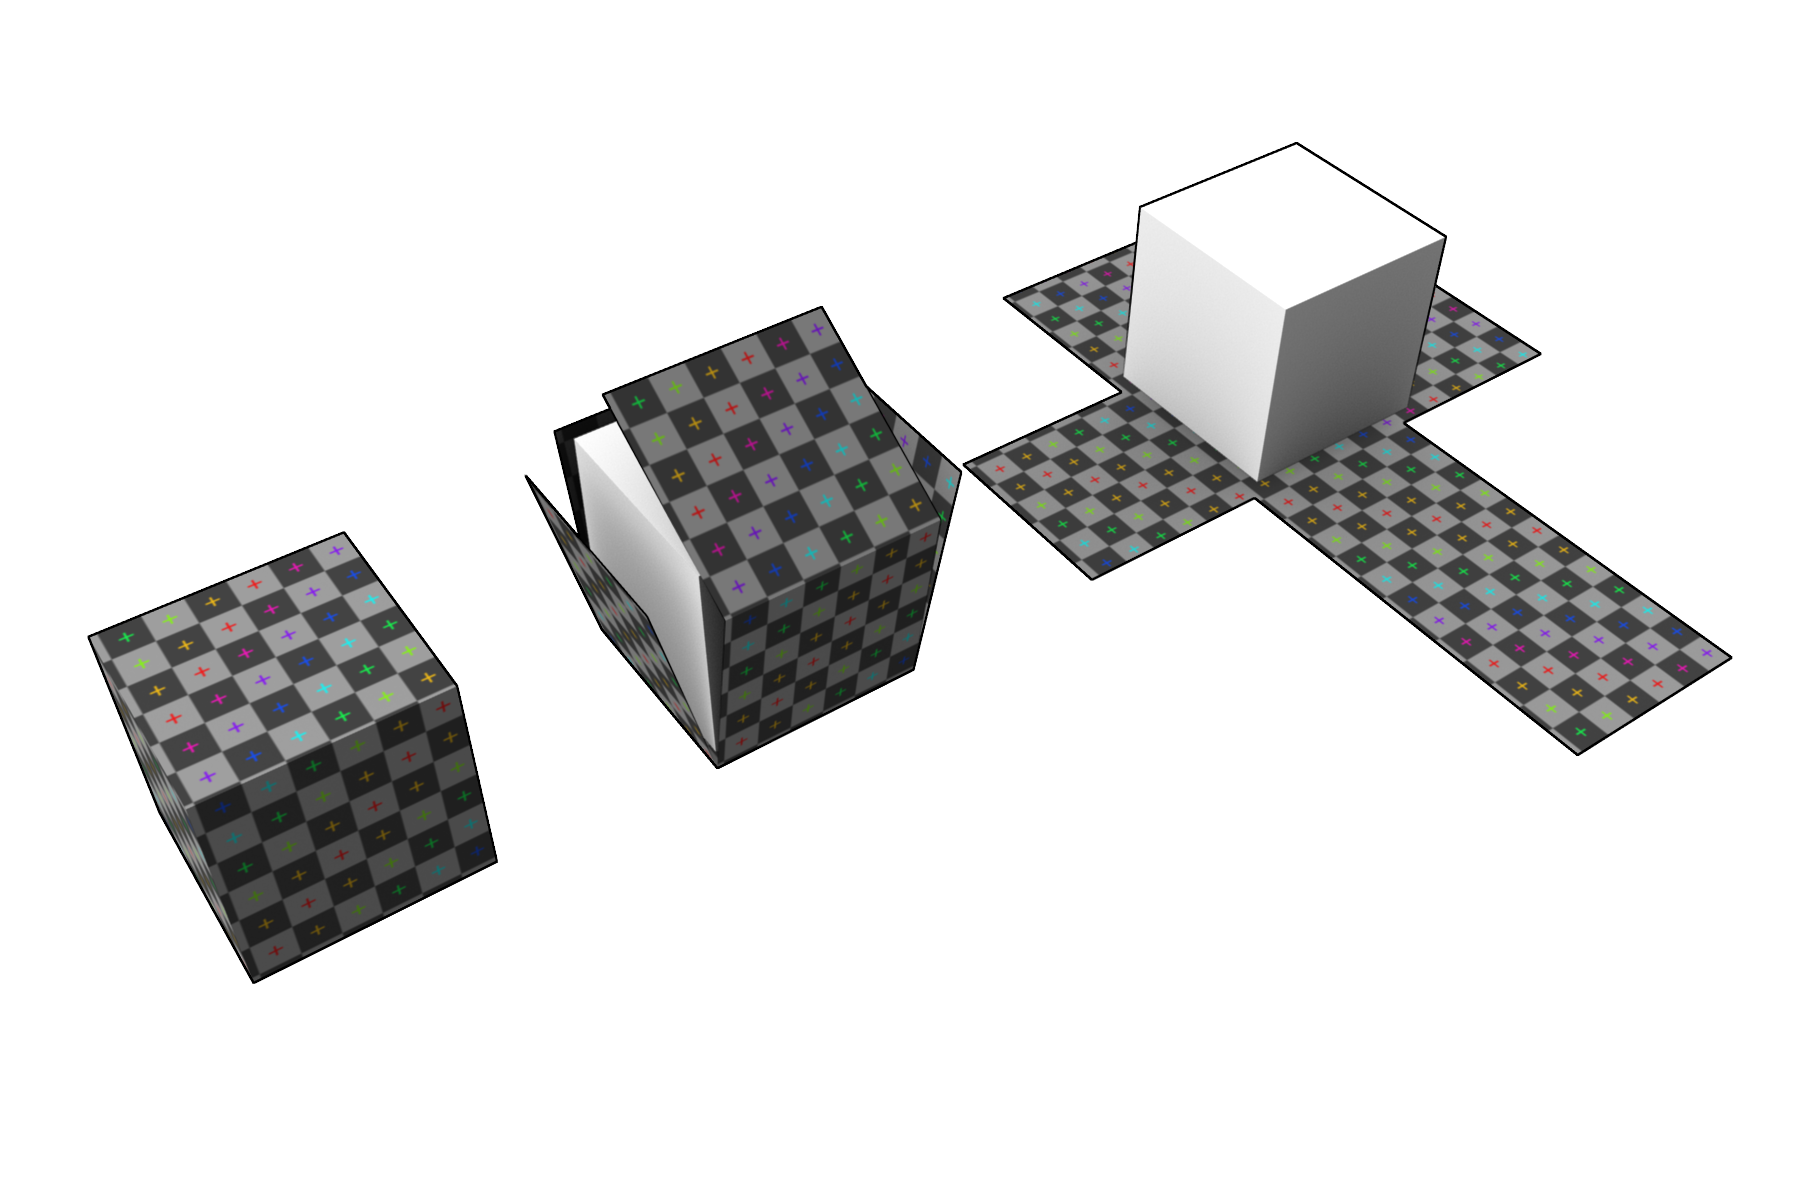
\includegraphics[width=.5\textwidth]{images/Technique/uvUnwrap.png}
	\caption{\label{fig:uvUnwrap}UV Unwrapping d'un cube {\cite{CubeRepresentativeUVUnwrapping_}}}
\end{figure}

Dans \nomJeu, tous les objets dont la couleur n'est pas simplement unie utilisent une texture de couleur. De même, les objets qui émettent de la lumière comme les enseignes lumineuses utilisent des \enquote{textures de rougeoiement} (\anglicisme{glow texture}). Les images sont créées dans GIMP, appliquées dans Blender par \anglicisme{UV unwrapping} et finalement exportées dans le moteur de jeu pour le rendu final.



\subsection{Highpoly vers Lowpoly}
\label{sec:highpolyVersLowpoly}
Le temps de calcul par image est un aspect très important lors de la réalisation d'un jeu vidéo. Trop élevé, il empêchera l'ordinateur d'afficher suffisamment d'images à la seconde pour rendre le flux vidéo fluide. Parmi les facteurs qui influent sur cette valeur critique, on notera principalement le nombre de sommets et de faces dans la scène. En effet, il faut calculer pour chaque face la position à l'écran des sommets (\textit{cf.} section \ref{section:calculMatriciel}), la quantité de couleur émise, les reflets, le z-index ou indice de profondeur\footnote{Le z-index décrit quelle est la face la plus proche de la caméra afin de n'afficher que cette dernière. Sans lui, ce serait la dernière face calculée qui serait affichée...}, etc.

Les objets utilisés doivent donc être les plus économes possible en matière de géométrie. Une technique très couramment utilisée pour diminuer le nombre de sommets avec un minimum de perte de qualité est celle du \anglicisme{normal mapping}.

On commence par réaliser un modèle très simplifié de l'objet. Ce dernier ne fera que rarement plus de 500 faces dans le cas d'un objet non-animé --- c'est le Lowpoly (\anglicisme{low}, bas ou peu; et \anglicisme{poly} pour polygone). On le duplique ensuite pour ajouter à la copie tous les détails désirés. Ce deuxième modèle peut posséder des millions de faces. Une fois cette opération terminée, on \enquote{cuit} (traduction littérale du terme anglais \anglicisme{bake} qui désigne cette manipulation) les différences de hauteur entre les deux objets sur une texture (\textit{cf.} section \ref{sec:textures}). Autrement dit, les différences de hauteur se trouvent renseignées sur une image 2D, codées en couleurs.

Il est possible de générer plusieurs types de texture: des \anglicisme{normal map} (pas vraiment de traduction) ou des \anglicisme{bump map} (\enquote{placage de relief} en français). Les premières sont codées en trois couleurs --- Rouge, Vert, Bleu --- soit trois informations qui représentent les translations sur les axes $X$, $Y$ et $Z$ de chaque point. La deuxième, plus simple, est une image en niveau de gris, soit à une seule dimension (le degré de noirceur) qui déterminera la translation de chaque point le long de la normale (\textit{cf.} section \ref{sec:normales}) de la face.

Ces textures sont appliquées sur l'objet Lowpoly. L'ordinateur calcule ensuite les ombres et certains détails comme si les sommets s'étaient réellement déplacés, donnant l'impression d'un niveau de détail très élevé bien que la géométrie de l'objet n'ait pas changé. Ceci permet, sans trop de perte de qualité, de faire passer le nombre de sommets par objet de plusieurs millions à quelques centaines seulement. Cette technique est très utilisée et on la retrouve dans tous les jeux vidéos modernes. Voir la figure \ref{fig:normalMapping} pour une illustration graphique du processus.

\begin{figure}[th!]
	\center
	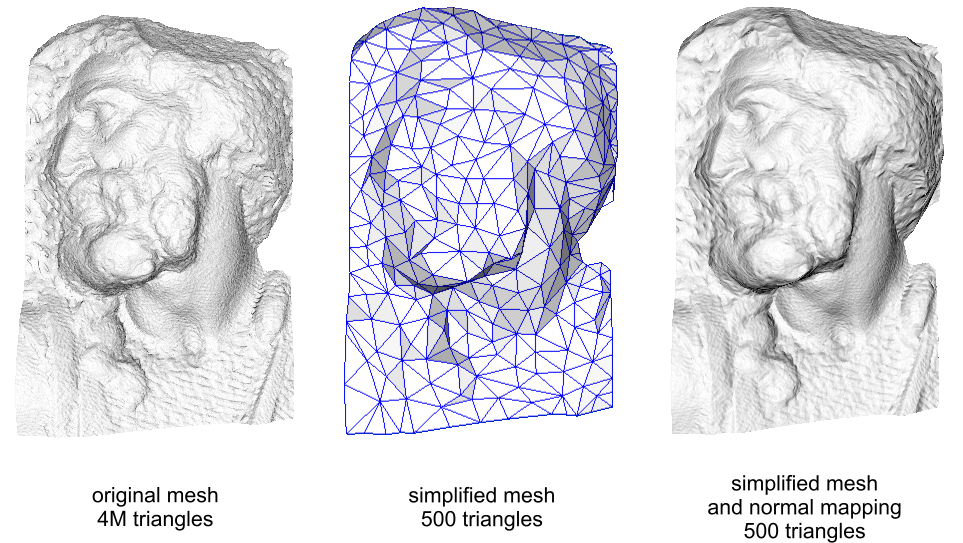
\includegraphics[width=.8\textwidth]{images/Technique/Normal_map_example.png}
	\caption{Exemple de \anglicisme{normal mapping\label{fig:normalMapping}} {\cite{Normalmappingusedtoredetailsimplifiedmeshes_}}}
\end{figure}


\subsection{Collision et \anglicisme{Raycast}}
\label{sec:collisions}
Si nous avons tous une perception intuitive des collisions avec la matière et de leurs effets dans la réalité, l'ordinateur n'a pas cette connaissance. Pour que l'univers virtuel devienne tangible, solide, il faut que l'ordinateur calcule les chocs et les conséquences qu'ils ont dans le jeu. Il faut donc ajouter pour chaque objet des \enquote{collisions}, soit une géométrie supplémentaire qui exécute du code lorsqu'un autre objet vient à la chevaucher. Il existe différents types de réponses possibles: l'objet peut ne pas bouger du tout, ricocher, faire ricocher l'autre, etc.

Une grande partie de ces calculs compliqués est prise en charge par le moteur physique de Godot. Il peut s'occuper de certains comportements par défaut comme les objets statiques ou ceux effectuant des mouvements simples. Mais les collisions d'un joueur, par exemple, sont nettement plus complexes à gérer: il faut qu'il puisse sauter, ce qui implique de la gravité (ajoutée par programmation); s'il y a des combats dans le jeu, le joueur doit pouvoir être touché et les dégâts éventuellement calculés en fonction du lieu d'impact, etc. Tout cela doit être codé à la main.

Le \anglicisme{Raycast} également nécessite des collisions pour pouvoir fonctionner. Cette technique permet de tirer un rayon\footnote{Aucun rayon n'est jamais tiré, c'est simplement une métaphore qui représente, dans la réalité, des calculs mathématiques.} depuis un objet ou l'écran et de voir quelle est la première géométrie de collision rencontrée. Cela permet de déterminer beaucoup de choses utiles: quel objet se trouve sous le curseur du joueur, l'ennemi peut-il détecter le joueur ou un mur bloque-t-il son champ de vision, etc.



\section{Code d'exemple --- Gestion de la caméra}

Dans un jeu vidéo à la première personne\footnote{Un jeu vidéo à la première personne est un jeu vidéo dans lequel le joueur est  le héros et voit par ses yeux. À l'inverse, dans un jeu vidéo à la troisième personne, le joueur voit le personnage qu'il contrôle; il est à l'extérieur du corps du personnage.}, l'orientation de la caméra est toujours gérée par l'utilisateur. Pour les jeux d'ordinateur, la souris est généralement affectée à cette tâche.

Il faut donc convertir les mouvements de la souris (translations 2D) en mouvements de caméra (rotations 3D). Les coordonnées $x$ de la souris détermineront les rotations horizontales (autour de l'axe $Y$) et les coordonnées $y$, celles verticales (autour de l'axe $X$). Toutes ces opérations doivent se faire sur le référentiel local de la caméra. Une implémentation simple est de coupler les déplacements de la souris sur les axes $X$ et $Y$ avec une rotation de la caméra autour des axes $Y$ et $X$:
\begin{align*}
		\delta x \cdot \kappa &= rotation_Y\\
		\delta y \cdot \kappa &= rotation_X
\end{align*}

Avec $\kappa$, le coefficient qui contrôle la vitesse de rotation de la caméra, et $\delta x$ et $\delta y$, les mouvements de la souris (considérés comme des angles en radians).

Cette implémentation est cependant incorrecte. On peut le voir avec l'exemple suivant:
\begin{enumerate}
	\item On fait une rotation verticale (selon l'axe local $X$) pour que la caméra regarde vers le haut avec un angle de 45°
	\item On fait pivoter la caméra horizontalement (selon l'axe local $Y$)
\end{enumerate}

L'étape numéro 2 va poser problème. En effet l'axe vertical local ($Y$) de la caméra a pivoté lors de l'étape 1 et fait un angle de 45°. Une rotation autour de cet axe aura pour conséquence de faire tourner la caméra \enquote{de biais}, donnant l'impression que la caméra tombe de son pivot. Un tel effet n'est évidemment pas désiré.

Il faut donc trouver une autre formule pour convertir les mouvements de la souris en rotation de caméra. Une bonne méthode consiste à les coupler aux angles polaires $\theta$ et $\varphi$ puis à utiliser la formule de conversion entre coordonnées sphériques et cartésiennes\cite{Coordonneesspheriques_}.

Les coordonnées sphériques servent à représenter des points dans l'espace (\textit{cf.} figure \ref{fig:coordonneesSpheriques}). Elles sont très souvent utilisées en cartographie. Les trois coordonnées sont données par:
\begin{itemize}
	\item Le rayon $\rho$ de la sphère sur laquelle se situe le point $P$ (soit la distance origine--point).
	\item Un angle horizontal, compris entre 0 et 2$\pi$, noté $\theta$
	\item Un angle vertical, compris entre 0 et $\pi$, noté $\varphi$
\end{itemize}
Ces coordonnées fonctionnent donc à l'aide de deux angles, exactement ce que les mouvements de la souris fournissent.

\begin{figure}[th!]
	\center
	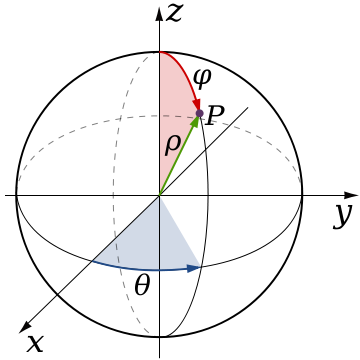
\includegraphics[width=5cm]{images/Technique/coordonneesSpheriques.png}
	\caption{\label{fig:coordonneesSpheriques}Coordonnées sphériques{\cite{Adiagramofsphericalcoordinatesdefiningapointbycolatitudelongitudeandradius_Wikipedia}}}
\end{figure}

Les coordonnées cartésiennes sont celles dont nous avons l'habitude, avec trois composantes: $x$, $y$ et $z$. La formule de conversion entre les deux systèmes est la suivante:
\begin{equation}
	\left\{
	\begin{array}{ll}
		x &= \rho \cos \theta\\
		y &= \rho \sin \theta \cos \varphi\\
		z &= \rho \sin \theta \sin \varphi
	\end{array}	
	\right.
	\label{eqn:coordonneesSpheriquesVersCartesiennes}
\end{equation}
Nous pouvons maintenant transformer les mouvements de la souris sur les axes $X$ et $Y$, en les couplant respectivement à $\theta$ et $\varphi$. Mais comment faire pivoter la caméra de la bonne façon avec de telles données?

Godot fournit une fonction --- \lstinline{Transform.looking_at(Vector3 point, Vector3 haut)} --- qui s'applique à un objet de type \lstinline{Transform} (qui représente un référentiel, \textit{cf.} section \ref{sec:referentiels}) et retourne une copie de ce référentiel mais pivoté de manière à ce qu'il regarde en direction de \lstinline{point}. Il ne reste plus qu'à calculer les coordonnées de \lstinline{point}. Pour ce faire, il faut ajouter aux coordonnées globales de la caméra le vecteur normalisé obtenu grâce à la formule \ref{eqn:coordonneesSpheriquesVersCartesiennes}. \lstinline{Point} se trouvera ainsi toujours dans une sphère de rayon 1 autour de la caméra qui le \enquote{suivra des yeux}.

\normalInfo{\lstinline{get_transform} et \lstinline{set_transform}}{Les méthodes \lstinline{get_transform} et \lstinline{set_transform} permettent respectivement d'obtenir et de définir le système de coordonnées locales d'un objet (orientation et position). C'est donc ces dernières qui sont utilisées pour faire pivoter la caméra.}

\renewcommand{\codeTitle}{Code de la caméra}
\begin{lstlisting}[caption=cameraControls.gd]
var view_sensitivity = 0.1
var angleHorizontal = 0 #angle horizontal de départ
var angleVertical = 90 #angle vertical de départ (droit devant)

func _ready(): #exécuté une fois au début
	set_transform(get_transform().looking_at(Vector3(0, 0, 1) + get_transform().origin, Vector3(0, 1, 0))) # définit le premier angle de la camera	
	
	Input.set_mouse_mode(2) #souris invisible, fixée au centre
	set_process_input(true) #la fonction _input sera exécutée à chaque fois que la caméra reçoit des inputs (dont les mouvements de souris)

func _input(ev): #cette fonction est exécutée à chaque fois que la souris bouge et gère la rotation de la caméra en fonction des mouvements de la souris
	if ev.type==InputEvent.MOUSE_MOTION:
		angleHorizontal = fmod(angleHorizontal + ev.relative_x * view_sensitivity, 360) #cette ligne ajoute à angleHorizontal le déplacement de la souris sur l'axe x multiplié par la sensibilité de la caméra puis retourne le reste de la division entière de angleHorizontal par 360 afin que cette variable ait toujours une valeur entre 0 et 360
		angleVertical = angleVertical + ev.relative_y * view_sensitivity #on ajoute à angleVertical le déplacement de la souris sur l'axe y multiplié par la sensibilité de la caméra
		
		#les quatre lignes suivantes empêchent angleVertical d'avoir une valeur supérieure à 180 ou inférieure à 0
		if angleVertical>180:
			angleVertical = 180
		if angleVertical<0:
			angleVertical = 0
		
		set_transform(get_transform().looking_at(where_to_look_at(angleHorizontal, angleVertical) + get_transform().origin, Vector3(0, 1, 0))) #cette ligne est très importante, elle change l'orientation de la caméra pour qu'elle pointe vers le point obtenu en ajoutant l'origine de la caméra au résultat de where_to_look_at

func where_to_look_at(theta_degré, phi_degré):
	var theta = deg2rad(theta_degré)
	var phi = deg2rad(phi_degré)
	var sin_theta = sin(theta)
	var sin_phi = sin(phi)
	
	return Vector3(sin_theta*sin_phi, cos(theta), -1 * sin_theta * cos(phi))
#c'est cette fonction qui fait la conversion entre coordonnées sphériques et cartésiennes C'est le coeur de l'algorithme. On remarquera d'ailleurs que la formule utilisée est la même que celle décrite juste au dessus
# (phi: 0°=regarde droit devant, positif a droite, negatif a gauche)
# (theta: 90°=regarde à l'horizontale, 0°=regarde en haut, 180=regarde en bas)
# Les angles doivent être compris entre -360 et 360 pour horizontal, entre 0 et 180 pour vertical
\end{lstlisting}


\section{Quelques problèmes rencontrés}

\begin{note}
	Cette section détaille quelques problèmes sur lesquels je suis tombé et donne des informations utiles pour mieux envisager le travail dans sa globalité. Elle ne se veut pas une liste exhaustive de tous les problèmes rencontrés, ce serait trop long.
\end{note}

\subsection{Les normales, de Sketchup à Blender}
La normale d'une face pointe normalement vers l'extérieure de cette dernière. Ainsi, un objet dont les normales seraient visibles ressemblerait à un hérisson (toutes les normales pointant vers l'extérieur de l'objet).

Afin de réaliser le moins de calculs possible, certains moteurs de jeu n'affichent que les faces qui pointent vers la caméra; à savoir, uniquement les faces dont la normale est orientée dans sa direction. Ceci permet, théoriquement, de diviser par deux le nombre de faces dont il faut faire le rendu et ainsi le temps de calcul pour une image. Bien que les cartes graphiques qui font ces calculs soient de plus en plus puissantes, beaucoup de moteurs de jeu utilisent ce procédé.

Godot n'est pas une exception. Il est également possible d'afficher toutes les faces, quelles que soient leur direction, mais cela n'est pas recommandé. En effet, pour que le jeu reste fluide, il faut au minimum 24 images par seconde (ou fps pour \anglicisme{Frame Per Second}) mais 60 est la norme recommandée pour que le joueur ne soit jamais dérangé par des images \enquote{sautantes}.

Cette spécificité des jeux vidéos ne pose généralement pas de problème. Par exemple, dans le cas d'objets modélisés dans Blender, étant donné que tout s'y fait à partir de formes primitives (cubes, cylindres, etc.) dont les faces sont bien orientées, la transition vers un moteur de jeu se fait sans problème. Mais prenons maintenant le cas d'objets importés de la 3D Warehouse de Google (\textit{cf.} section \ref{sec:modelisationContenu3D}) puis convertis pour Blender. Le programme utilisé par défaut pour le visionnement et l'édition des fichiers de la librairie en ligne, Google SketchUp, n'est pas (ou peu) sensible à l'orientation des faces. Ainsi, certains modèles arrivent dans Blender avec une partie de leurs normales mal orientées... Mais Blender n'est pas touché par ce problème: tout comme Google SketchUp, il affiche toutes les faces, quelle que soit leur disposition. C'est au moment de passer l'objet dans le moteur de jeu que la moitié des faces disparaissent, car ce programme, lui,  est sensible à la direction des normales!

Un objet, dans cet état, est inutilisable dans le moteur de jeu. Deux solutions s'offrent alors: inverser à la main ou de façon semi-automatisée les faces dans Blender, ce qui représente un travail long et fastidieux. Ou alors, changer carrément d'objet, par exemple en le modélisant à la main. Heureusement, tous les fichiers ne présentent pas ce genre de difficultés. Mais ceux qui en souffrent  sont souvent irrécupérables et font perdre un temps précieux. De plus, ce problème, lorsqu'il est rencontré pour la première fois surprend beaucoup (et peut causer un certain énervement).


\subsection{Importation des textures dans Godot}
Blender dispose d'une interface très puissante pour créer des matériaux. Il est possible d'en inventer une grande quantité, pouvant ressembler à n'importe quelle matière réelle. Le nombre d'options configurables est tout simplement affolant. Pas étonnant que les matériaux soient une des difficultés majeures de ce programme qui effraie encore et toujours les novices (moi compris).

Godot est écrit de façon à être compatible avec Blender. Cependant, n'ayant pas encore atteint un niveau élevé de maturité, nombreux sont encore les bugs concernant l'importation de textures. De fait, ces dernières devraient normalement être créées directement dans le moteur de jeu pour éviter tout problème. Il est cependant impossible de remplir une telle exigence dès que l'on désire utiliser des textures de couleurs ou des normales map (par opposition aux \enquote{textures procédurales}), l'\anglicisme{UV unwrapping} devant se faire avec Blender. De plus, la plupart des objets provenant de la 3D Warehouse sont déjà texturés. N'oublions pas non plus que les multiples conversions de format entre Google Sketchup et Blender puis entre Blender et Godot ne facilitent pas la transition.

À de multiples reprises, les objets sont arrivés gris (couleur par défaut $\rightarrow$ texture non importée) dans le moteur de jeu. Il m'aura fallu beaucoup de temps pour comprendre la source du problème (pour être plus exact, \textit{les} sources du problème).

Utilisant de multiples répétitions du même objet dans Blender, j'ai créé des références vers ces objets dans mes scènes, plutôt que de copier chaque objet dont j'avais besoin. De cette façon, si je modifiais l'objet, il changeait également dans toutes les scènes où il était référencé. C'est une façon de dire à Blender \enquote{Mets l'objet \textit{x} à cet endroit dans la scène. Pour trouver les données de cet objet, ouvre le fichier \textit{xxx.blend}.} Si l'idée paraissait excellente, il s'est avéré que l'exporteur ne supporte pas cette option et retourne une erreur relative aux textures.

Ce premier problème me causa beaucoup de soucis conjointement avec un autre. En effet, une fois la question de l'importateur réglée et l'objet importé, les textures apparaissaient grises. Elles n'avaient donc pas été importées. Cela provenait du fait que Godot stocke dans le cache (garde en mémoire) les textures qu'il a déjà copié à l'importation précédente. Modifier ces textures, à moins de réimporter l'objet complètement, n'a donc pas d'effet dans le moteur de jeu.

La combinaison déroutante de ces deux bugs me coûta plusieurs heures avant d'être résolu correctement (enfin je crois... J'ai, de fait, toujours des problèmes avec cette importation).

\subsection{Animation des personnages}
Modéliser un humain représente un véritable casse-tête. La complexité du corps est telle qu'il est impossible d'obtenir un résultat satisfaisant sans passer des jours derrière l'écran. Ainsi, j'ai décidé d'utiliser MakeHuman, un logiciel libre et gratuit, pour créer mes personnages. Ce programme propose une interface très complète pour créer des êtres humains de toutes sortes, toutes les couleurs de peau, toutes les corpulences, etc. Un modèle spécial jeu vidéo est proposé, contenant beaucoup moins de sommets afin de soulager le processeur d'une surcharge de calculs. Enfin l'importation dans Blender est quasiment transparente et pose généralement peu de difficultés.

Celles-ci se présentent au moment d'animer le personnage. Les techniques d'animation modernes requièrent un studio, des acteurs, des caméras 3D et une grosse puissance de calcul (les mouvements des acteurs sont immédiatement appliqués aux personnages en 3 dimensions). Cette technique était bien sûr exclue d'office pour moi. Autre possibilité, tout modéliser à la main. Mais, une fois de plus, l'univers de l'animation est très particulier et pour arriver à un résultat convaincant, des centaines d'heures sont probablement nécessaires. Une cinématique \enquote{aussi simple} que la marche est très difficile à modéliser pour paraître réaliste et fluide.

La solution était donc de trouver sur internet des fichiers contenant déjà la digitalisation d'animations capturées avec les méthodes professionnelles. Et de tels fichiers existent. Ils sont même relativement répandus.

Mais les vrais ennuis arrivent au moment d'appliquer ces animations aux personnages. Les fichiers contiennent les modifications à appliquer à chaque os de l'armature contrôlant la géométrie du personnage\footnote{Les géométries compliquées, pour simplifier leur animation, sont contrôlées grâce à des \enquote{os}. Ce sont des entités auxquelles sont attribués certains sommets de la géométrie de l'objet. Ainsi en faisant bouger un os, tous les sommets qui lui sont liés bougent simultanément.} sur chacun des axes à chaque image. On voit immédiatement les multiples complications qui peuvent apparaître: comment faire si le nombre d'images par seconde dans le fichier n'est pas le même que dans Blender? Les animations se dérouleront au ralenti ou en accéléré. Et que faire si l'armature utilisée dans le fichier d'animation n'est pas la même que celle de l'objet à animer?

Pour cela, l'addon MakeWalk de Blender est simplement impressionnant. Il est capable de modifier la vitesse de l'animation seul, mais mieux encore, il est capable de comprendre quels os de l'animation représentent quels os du personnage! Cependant, un processus d'une telle complexité ne peut toujours réussir. Ainsi il n'est pas rare d'avoir des problèmes mineurs mais cependant dérangeants dans les animations. Par exemple, l'animation \enquote{marcher}, une fois appliquée, causait aux personnages d'avoir les chevilles et les pieds étrangement orientés vers l'intérieur.

Il a donc fallu jouer avec les options de configuration de MakeWalk, comprendre les possibilités qu'il offre, etc.


%\chapter{Diffuser un jeu libre}
%\printMiniToc


\chapter{Pour conclure}
\printMiniToc

\section{Diffusion}
Si \nomJeu\ vient un jour à être distribué, ce sera gratuitement et librement, bien sûr! Chacun pourra télécharger le jeu et l'essayer sans payer. Mais plus encore, chacun sera libre de télécharger et modifier son contenu puis de le redistribuer (sous la même licence). Il pourrait même être envisageable de rendre le jeu public avant qu'il ne soit achevé et demander de l'aide à la communauté pour le terminer mais cela implique beaucoup de coordination et une certaine perte de contrôle sur la version \textit{officielle} du jeu.


\section{Réaliser un jeu vidéo libre?}
Pour la réalisation de ce jeu, je m'étais fixé comme condition de n'utiliser que des logiciels gratuits. Atteindre cet objectif fut relativement simple. Il existe, de par le Net, une multitude de programmes gratuits et c'est sans difficulté que j'ai trouvé les outils qui m'étaient nécessaires.

Pour ce qui est du deuxième objectif, à savoir utiliser le plus possible de logiciels libres, je fus agréablement surpris de constater qu'ils sont également nombreux et divers. En effet, il existe, pour la plupart des tâches que nécessite la création d'un jeu, des outils open source. Un seul programme a fait exception à la règle pour \nomJeu: Sketchup. J'avais besoin de ce dernier pour convertir les modèles téléchargés d'Internet vers des formats plus aisément éditables. Impossible de s'en passer donc et impossible de trouver une alternative. Mais ce n'est qu'une goutte au milieu de l'océan.

À mon avis, les objectifs fixés au début de ce document concernant l'aspect technique sont atteints. C'est pour moi la preuve qu'Internet pourrait apporter une révolution dans notre mode de fonctionner: un monde où \textit{la communauté} revêtirait une importance toute particulière, où l'information serait libre et gratuite et où les outils seraient disponibles pour tous ceux qui en auraient besoin.


\section{Réaliser un jeu vidéo seul?}
La création d'un jeu vidéo se déroule principalement en deux étapes que la structure de ce TM  reflète: la préparation sur le papier du design, du scénario, des personnages, etc. puis la réalisation technique avec ses contraintes et problèmes. Commencer un jeu sans idée claire de la direction qu'il va prendre est la meilleure façon de faire beaucoup de travail inutile et de ne jamais aboutir à rien.

Mon scénario n'est bien sûr pas terminé. Cependant, je pense qu'il est suffisamment détaillé pour permettre la création des premiers niveaux. Il pose en tout cas les bases du gameplay, des personnages et dans une moindre mesure l'apparence d'Éluria. Il m'aura fallu pas mal de temps pour en arriver là: le scénario n'a vraiment pris forme que durant l'été. Mais cette réflexion m'a été très utile pour arriver à un tout cohérent et conforme aux buts que je voulais donner à mon jeu. Par exemple, éliminer l'aspect violent peut se révéler être très difficile.

L'expérience fut moins concluante du point de vue de la réalisation technique. S'il était évident que je ne pouvais finir un jeu complet en moins d'une année, j'aurais aimé mener ce projet plus loin, dans le temps imparti. Certaines tâches qui me semblaient aisées de prime abord m'ont parfois demandé des heures de recherches et certains \anglicisme{bugs} m'ont coûté un temps important et précieux. Mais plus encore, je remarque que certaines tâches très chronophages de ce travail, tel l'apprentissage des règles et du langage de Godot n'apparaissent pas dans le résultat final. C'est, d'une certaine façon, la partie immergée de l'iceberg, et ces nécessités représentent la part ingrate de ce travail car rares sont les personnes qui mesurent l'engagement nécessaire pour accomplir ces tâches.

Je rends donc un scénario conforme à mes espérances mais une esquisse du jeu moins avancée que ce que j'espérais. Cependant, les bases sont posées. Le scénario est défini dans les grandes lignes et le code de base du jeu est écrit. Mon Travail de Maturité se termine, ce n'est pas le cas du projet \nomJeu. Mon intention est de continuer ce jeu et qui sait, dans quelques années, de le publier si j'arrive un jour à le terminer.


\section{Bilan personnel}
Ce Travail de Maturité fut pour le moins riche en expériences, certaines très positives, d'autres moins. Pour être honnête, il fut pour moi source de stress; j'aurais voulu porter la réalisation du jeu plus loin, ajouter plus de détails, de fonctionnalités. S'engager dans un travail d'une telle ampleur avec la volonté de le mener à bout peut causer des tensions considérables, surtout au vu des difficultés qu'a pu représenter cet objectif.

Évidemment, l'informatique ne serait pas une si belle science sans la part d'énervement qui vient avec. Au cours de cet exercice, combien de fois n'ai-je pas pesté contre les circuits de cette machine tellement complexe qu'est l'ordinateur. Parfois très frustrantes, les contrariétés qui formèrent tout de même la plus grande partie de ce travail furent d'incessantes sources d'irritation.

Il m'a parfois fallu faire de gros efforts pour rester motivé. Apprendre le fonctionnement de Godot (vous trouverez, pour vous faire une idée de sa taille, la documentation du moteur de jeu à l'adresse \url{https://github.com/okamstudio/godot/wiki}) fut probablement un premier obstacle. Mais je suppose que le pire fut la modélisation. Les nombreux problèmes, souvent peu ou mal documentés, rencontrés durant cette étape furent autant de sources de démotivation: bugs de textures, sommets dupliqués, difficultés à trouver des convertisseurs entre Sketchup et Blender, problèmes avec les formats de fichier à l'exportation de Blender vers Godot, objets trop lourds faisant surchauffer le moteur de jeu, création et exportation des animations des personnages; la liste est encore longue.

Mais il est évident que ce travail m'a aussi beaucoup apporté. J'ai dû persévérer malgré les difficultés et l'énervement. Ce fut aussi l'occasion d'acquérir toutes sortes de connaissances techniques. Dans l'univers de l'informatique et de la création 3D bien sûr, mais aussi dans d'autres domaines plus variés comme l'édition de son et la création de cartes géographiques (et toutes les mathématiques associées à ce dernier thème).

Cet écrit représenta une opportunité pour moi d'exercer une autre de mes passions, la typographie. Réalisé avec \XeLaTeX, un langage de description très puissant, la mise en page de ce document fut une sorte de laboratoire d'essai, l'occasion d'en découvrir (beaucoup) plus sur ce programme fantastique, développé dans les années 80 et pourtant si actuel dans l'univers rapidement changeant de la technologie, qu'est \TeX\ (\XeLaTeX\ étant une sur-couche de \LaTeX\ (développé par Leslie Lamport), lui-même une sur-couche de \TeX\ (développé par Donald Knuth)). J'ai pris beaucoup de plaisir à faire des recherches à ce sujet, choisir des fontes adaptées, créer des tableaux, de même qu'une configuration de page très particulière et des débuts de chapitre un peu fous.

J'ai aussi découvert l'univers du game designer, je suis en quelque sorte passé de l'autre côté du miroir. De joueur, je suis devenu créateur et je n'en apprécie que plus les jeux réussis tant graphiquement que du point de vue du scénario. Ce fut aussi l'occasion de mieux envisager la dichotomie du processus de création d'un jeu: l'aspect purement créatif et ses idées folles souvent peu réalisables, et le point de vue technique de l'informaticien, qui tous deux furent mes réalités à différents moments.

La création d'un univers, outre son aspect fortement divertissant, m'a permis d'en apprendre plus sur mes propres processus créatifs. Mais peut-être plus important encore, ce premier aperçu de la création d'un univers, cet exercice d'imagination m'a donné la chance d'apprendre à me connaître. Les sujets importants pour moi, les personnages que j'ai créés, l'histoire telle que je l'ai conçue; tous ces éléments, finalement, sont des reflets de mes valeurs et me permettent de me découvrir.





\appendices
\renewcommand{\thecontentspage}{Annexe}
\startcontents[chapters]
\chapter{Glossaire}

\newpage

\label{chap:vocabulaire}
\begin{center}
	\begin{longtabu} to \textwidth {l >{\bfseries}X[r, 1] X[4] l}
		\rowfont{\bfseries\sffamily\leavevmode\color{white}}
		\rowcolor{mainColor}
		& Mot & Définition & \\
		\endhead
		\endfoot
		%
		& Add-on & Un add-on, ou plug-in, est un morceau de code qui est ajouté à un programme afin de lui ajouter une ou plusieurs fonctionnalités spécifiques qui ne sont pas fournies par défaut. & \\
		%
		& Boss & Anglicisme qui désigne l'ennemi principal du jeu ou du niveau. Il peut y avoir plusieurs boss s'ils sont propres aux niveaux. Ces personnages sont, en général, rencontrés en combat au moins une fois. L'exemple le plus connu est \enquote{Bowser}, un dragon diabolique, qui enlève la belle \enquote{Peach} dans le jeu \enquote{Mario} & \\
		%
		& Démo & Abbréviation de \enquote{version de démonstration}; désigne une version incomplète d'un jeu vidéo. Il peut s'agir d'un nombre diminué de niveaux, de possibilités de jeu bridées ou de toute autre méthode réduisant la version intégrale du jeu. & \\
		%
		& Gameplay & Anglicisme désignant la façon dont le joueur peu interagir avec le jeu, les actions qui lui sont permises, les objets qui sont à sa disposition, les façons de faire permettant de surmonter les défis du jeu, etc. & \\
		%
		& HUD & Acronyme de \textit{Head-Up Display}. C'est toute l'interface 2D présente sur l'écran du joueur alors qu'il est dans le jeu (vraiment en train de jouer, pas les menus). Cela peut comprendre par exemple la barre de vie, l'argent disponible, les armes équipées ou encore la minimap. Ce sont des informations qui apparaissent comme s'il y avait une vitre devant vos yeux sur laquelle on projetait des images. Initialement, cela désignait bien des vitres sur lesquelles étaient projetées des informations de vol... dans les cockpit des avions de chasse. & \\
		%
		& Moteur de jeu & Un moteur de jeu est un programme chargé de centraliser plusieurs aspects de la création de jeu vidéo: importation de contenu (3D ou 2D), calculs pour le rendu des images (dans le cas d'un univers en 3D: projection de cet environnement sur un espace 2D -- l'écran), gestion du son, programmation des actions ou des personnages (ou scripting), exportation vers diverses plateformes, etc. & \\
		%
		& Open-world & Anglicisme; littéralement \enquote{monde ouvert}. Désigne un jeu vidéo dans lequel le joueur peut se déplacer librement à travers un univers virtuel très vaste. Il y dispose d'une grande liberté d'action. & \\
		%
		& PNJ & Abréviation tirée du domaine du jeu de rôle, signifiant Personnage Non Joueur, soit n'importe quel personnage qui n'est pas contrôlé par un homme. Ils désignent, dans un jeu vidéo, les protagonistes de l'histoire contrôlés par l'ordinateur. & \\
		%
		& Puzzle & Une énigme, une devinette ou un mini-jeux à résoudre pour pouvoir avancer dans le jeu, débloquer des trésors cachés ou encore compléter des objectifs secondaires. Ils peuvent être de formes très diverses: épreuve de rapidité, d'adresse, de réflexion, etc. Par exemple, dans le jeu \textit{The Legend of Zelda: Spirit Tracks} il faut reproduire un morceau de musique avec un instrument débloqué au fil de l'aventure pour accéder à certains lieux. & \\
		%
		& Screenshot & Anglicisme signifiant \enquote{capture d'écran}; autrement dit, une photo de ce qui s'affiche à l'écran. & \\
		%
		& Semi open-world & De l'anglais, \enquote{monde semi-ouvert}. C'est un niveau ou type de jeu dans lequel le joueur est libre de ses mouvements. Cependant des éléments du décor limitent la taille de l'univers. On trouvera, par exemple, des îles (la mer est l'élément bloquant), des villes fortifiées (les murailles sont les éléments bloquants) ou encore une maison dont on ne peut sortir. Les niveaux de type \anglicisme{alley} désigne exactement la même chose mais semi open-world ou open-world sont des termes que l'on peut entendre en français. Voir également la définition de \enquote{Open-world} & \\
		%
		& Succès & Traduction de \anglicisme{achievement}, ce sont des récompenses honorifiques attribuées au joueur à l'accomplissement d'un tâche donnée, d'objectifs supplémentaires, etc. & \\
		%
		& Story-telling & Anglicisme; décrit l'art de raconter une histoire efficacement. Cela inclut par exemple: le point de vue narratif, l'intrigue, les personnages mais aussi l'intonation, les gestes, etc. Dans le cadre d'un jeu vidéo, cela décrira les techniques narratives, les libertés laissées au joueur, etc. & \\
		%
		& Temple & Un temple fait référence, dans l'univers du jeu vidéo, au dernier niveau d'un chapitre ou acte du jeu. Il se déroule généralement dans l'entre de l'ennemi principal ou tout du moins d'un adversaire de grande importance. Ce type de niveau se conclu généralement par un affrontement entre le joueur et l'ennemi cité avant -- appelé alors boss. On citera ainsi Super Mario Bros dans lequel chaque dernier niveau se déroule dans un château de Bowser ou encore Zelda où chaque temple conclu une partie du jeu et coïncide généralement avec l'obtention d'un nouvel objet. & \\
		%
		& Workflow & Anglicisme, que l'on pourrait traduire par \enquote{flux de travail}. Cela désigne l'ensemble des étapes que vont subir des informations, des documents ou des produits pour passer d'un premier état à un deuxième. & \\
	\end{longtabu}
\end{center}


\chapter{Steampunk}
\newpage

\label{app:steampunk}
\section{Définition}
Selon Wikipédia: \enquote{L'expression steampunk, qui signifie littéralement \enquote{punk à vapeur}, parfois traduite par \enquote{futur à vapeur}, est un terme inventé pour qualifier un genre de littérature né à la fin du XXe siècle, dont l'action se déroule dans l'atmosphère de la société industrielle du XIXe siècle. Le terme fait référence à l'utilisation massive des machines à vapeur au début de la révolution industrielle puis à l'époque victorienne. Aujourd'hui le steampunk est considéré comme un esthétisme pouvant intéresser à la fois des œuvres littéraire fantastique, de fantasy, d'anticipation et certains sous-genres de la science-fiction.}\cite{Steampunk_}

D'autres définissent ce genre comme étant: \enquote{la technologie moderne -- iPads, ordinateurs, robots, avions -- alimentée par la vapeur et insérée dans le 18\textsuperscript{e} siècle}.\cite{Whatissteampunk_}

Le Steampunk est un des univers fantastiques que j'apprécie le plus, il regroupe en même temps science-fiction, fantaisie et caractéristiques rétros. Il possède à la fois un côté technologique et une ambiance sombre qui en font un environnement mystérieusement attirant.

\newpage
\section{Quelques images}
\vspace*{-.5cm}
\begin{minipage}{.49\textwidth}
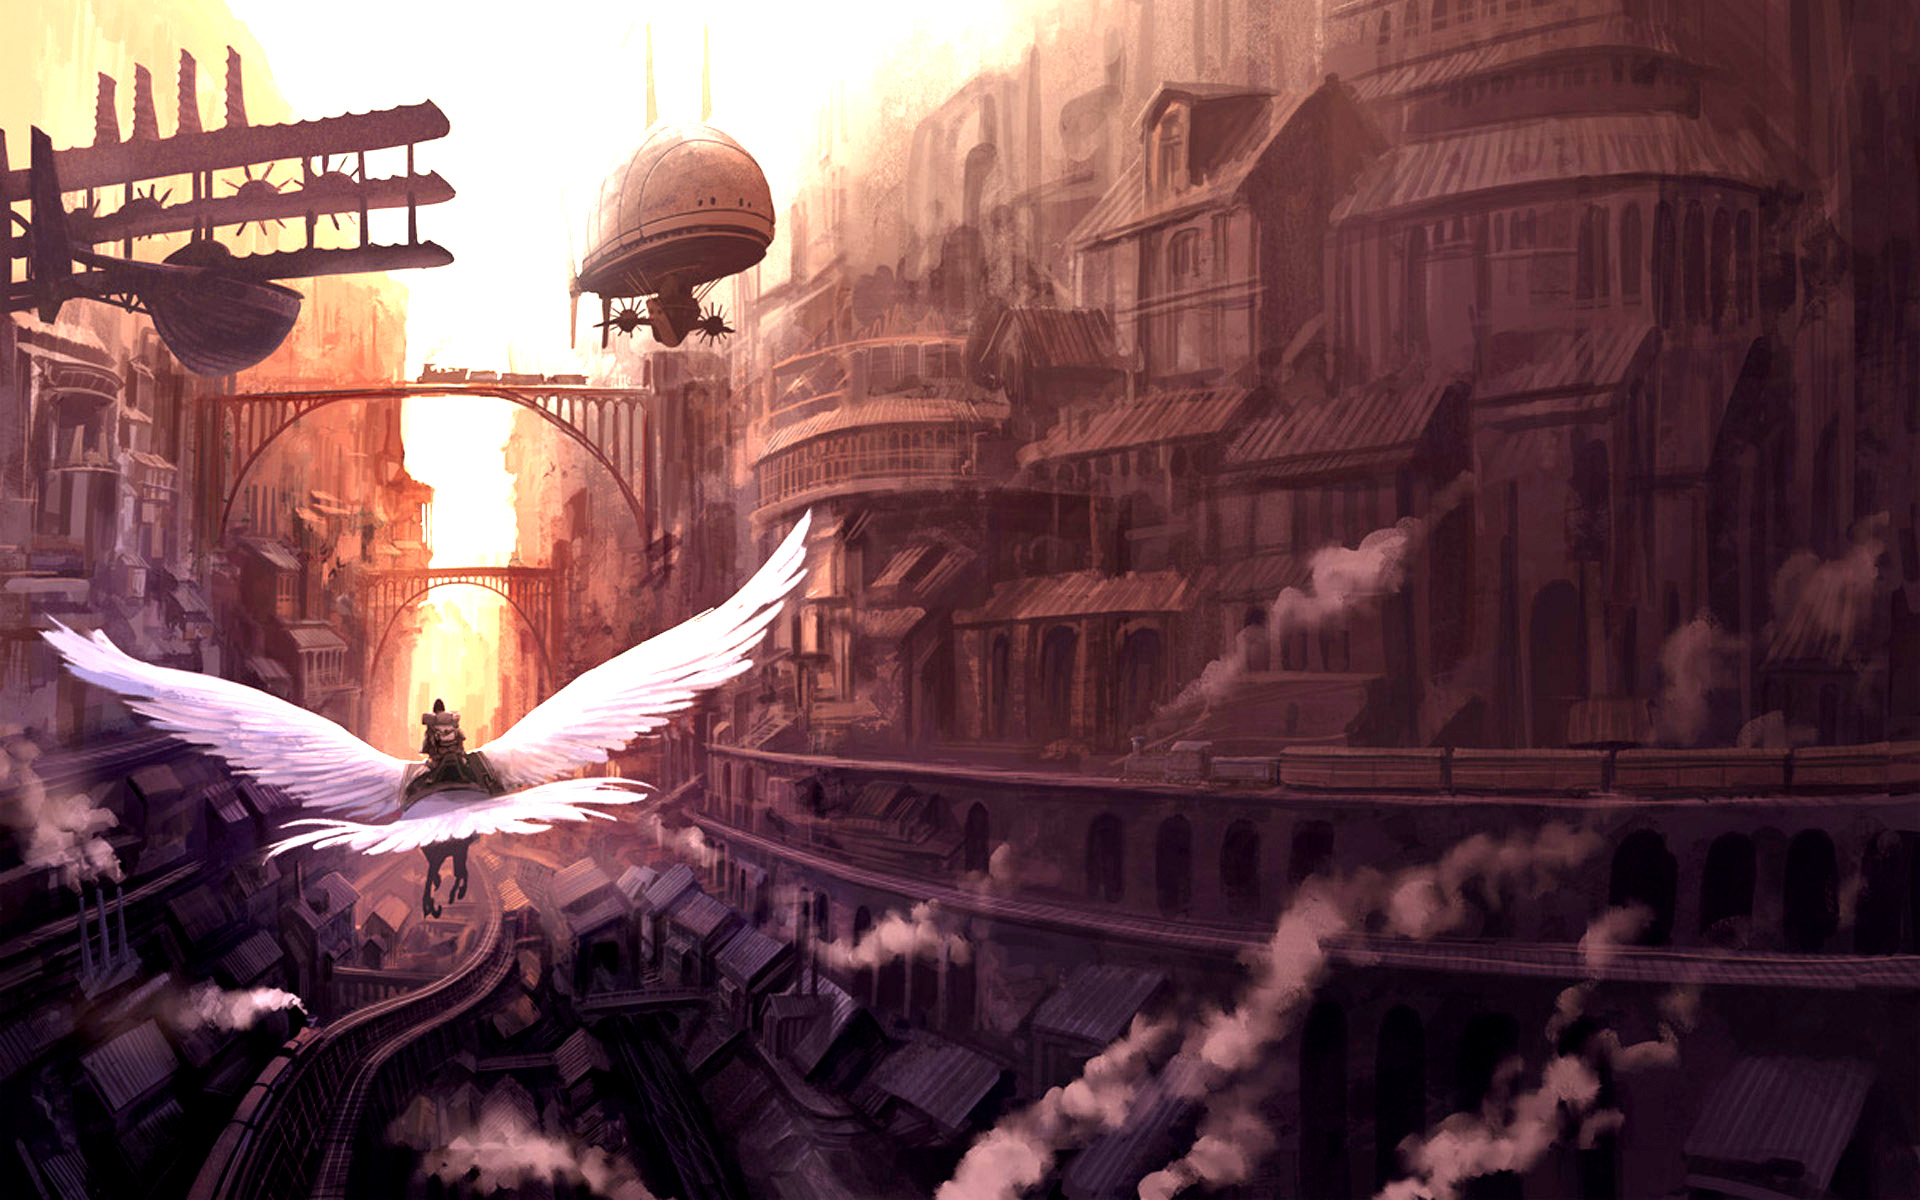
\includegraphics[width=\linewidth]{./images./Annexes/Above-the-city-steampunk-wallpaper.jpg}
\\[-1mm]\citeurl{AboveCityWallpaperSteampunkWallpaper_Matt69ers_sl}
\end{minipage}
\hspace{.02\textwidth}
\begin{minipage}{.49\textwidth}
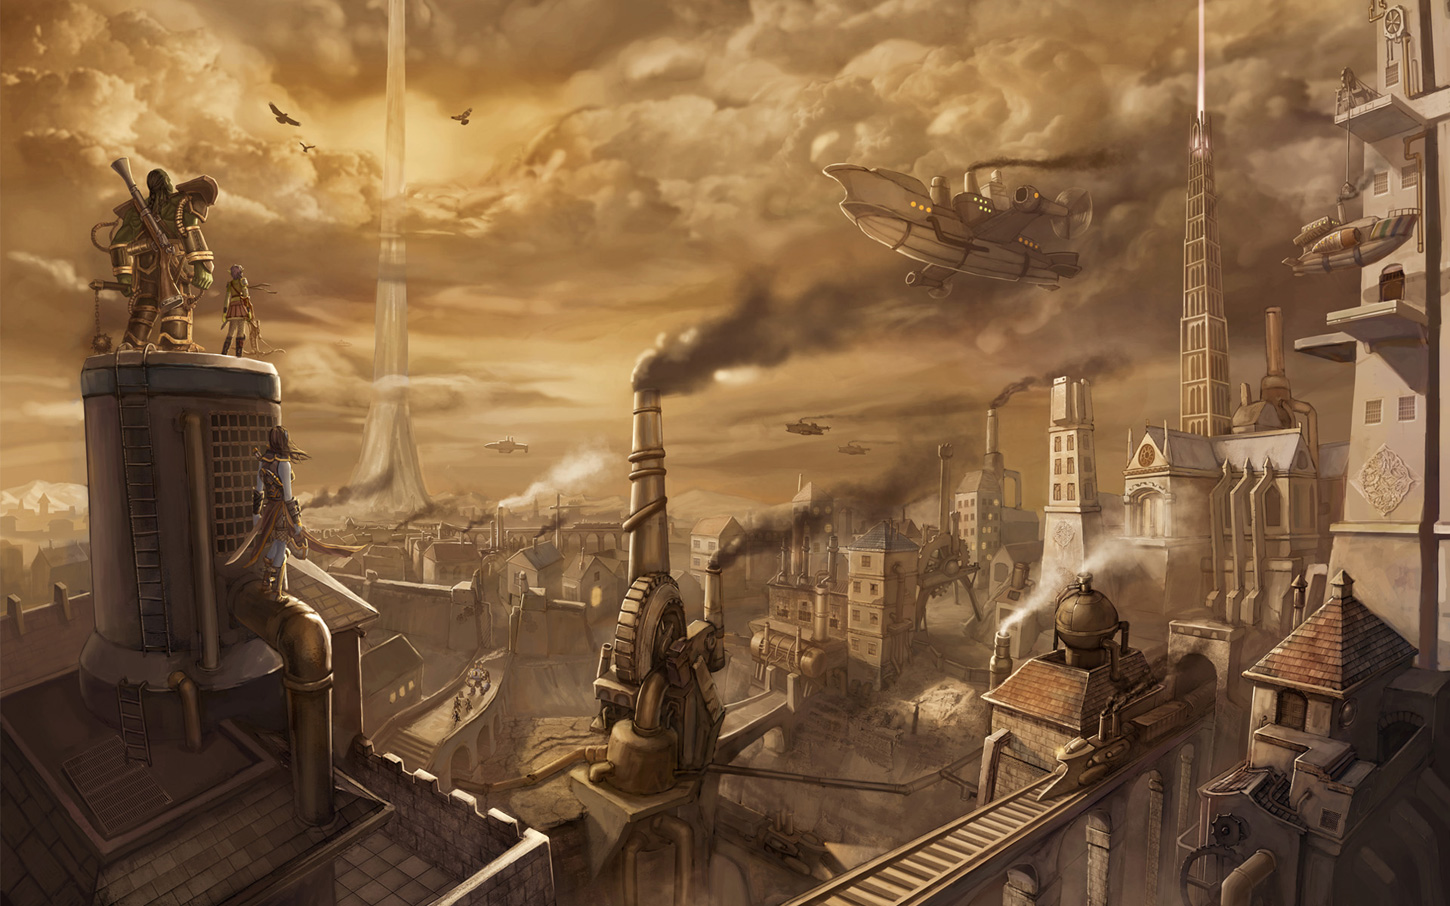
\includegraphics[width=\linewidth]{./images./Annexes/city-of-steam-steampunk.jpg}
\\[-1mm]\citeurl{CityofSteamAcikBetaBasliyor_}
\end{minipage}

\begin{minipage}{.49\textwidth}
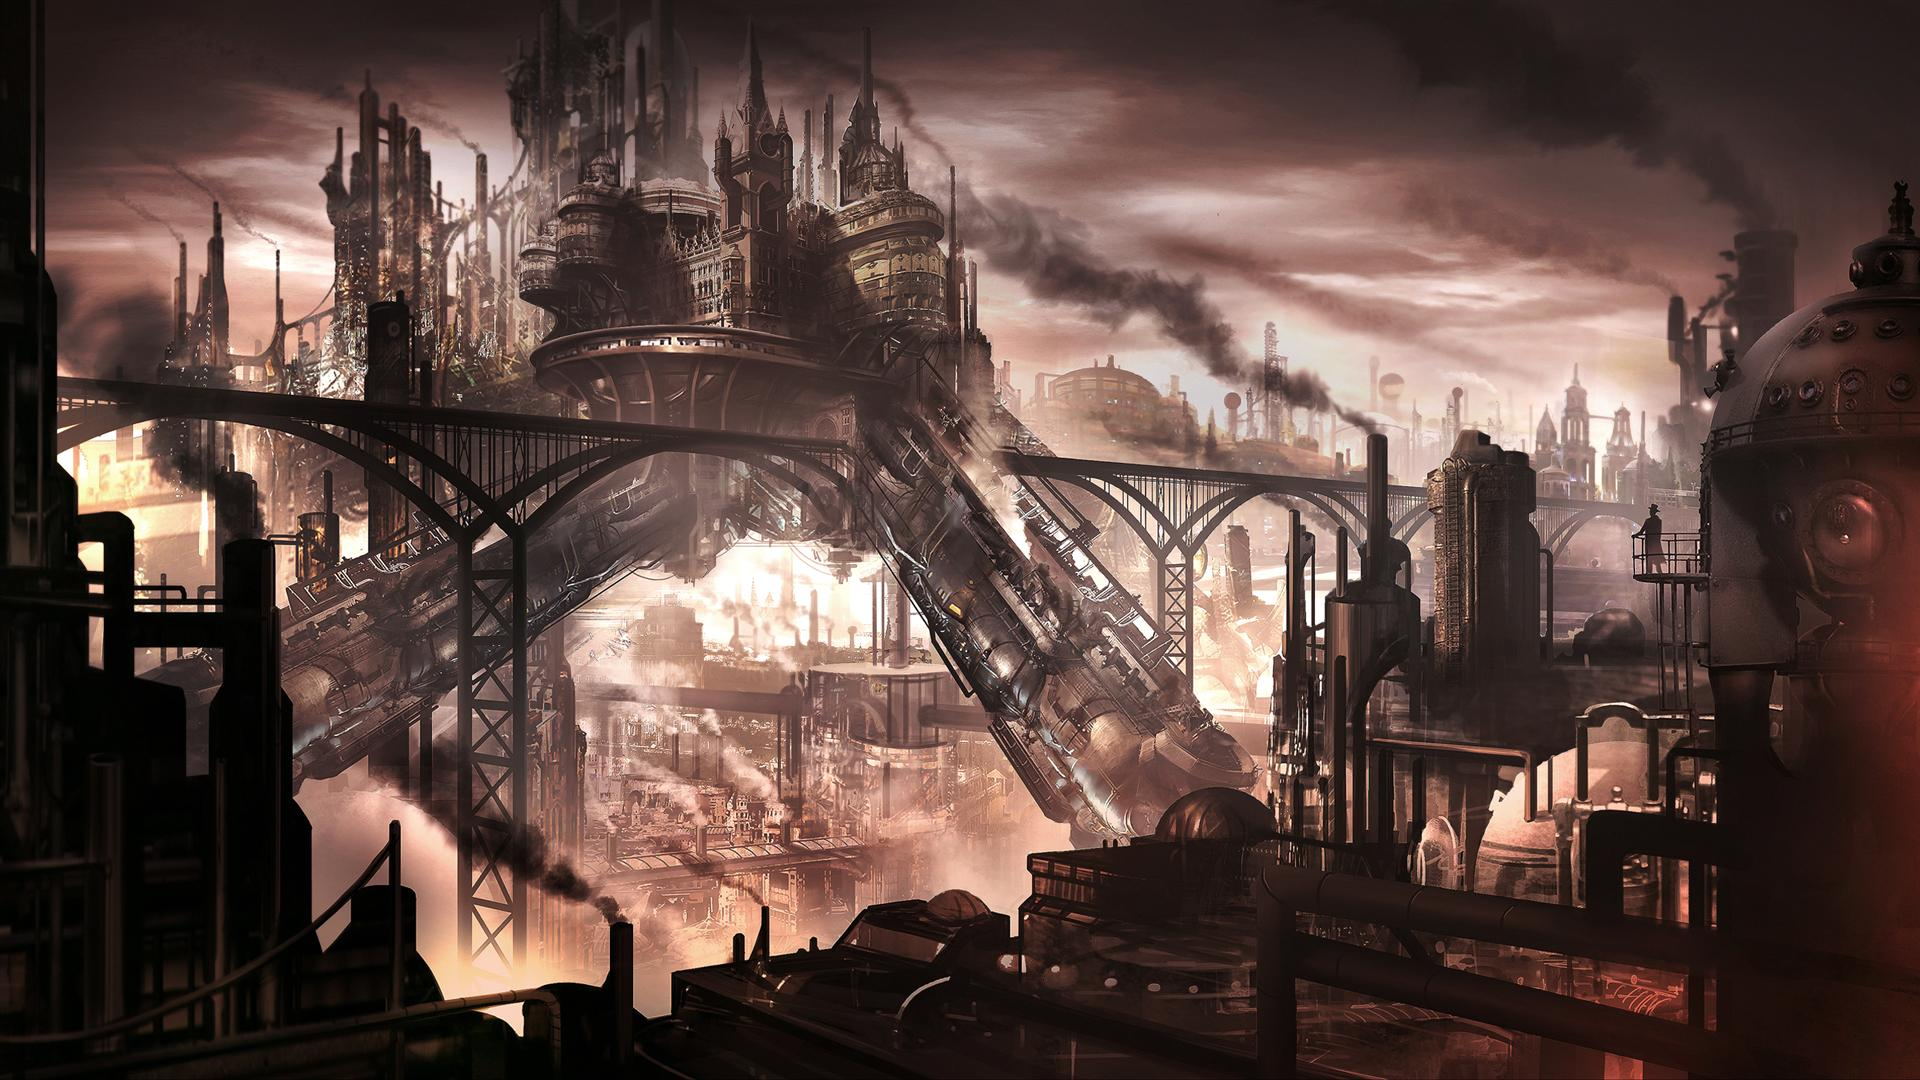
\includegraphics[width=\linewidth]{./images./Annexes/concept_001.jpg}
\\[-1mm]\citeurl{SteampunkTeslapunkonPinterest_}
\end{minipage}
\hspace{.02\textwidth}
\begin{minipage}{.49\textwidth}
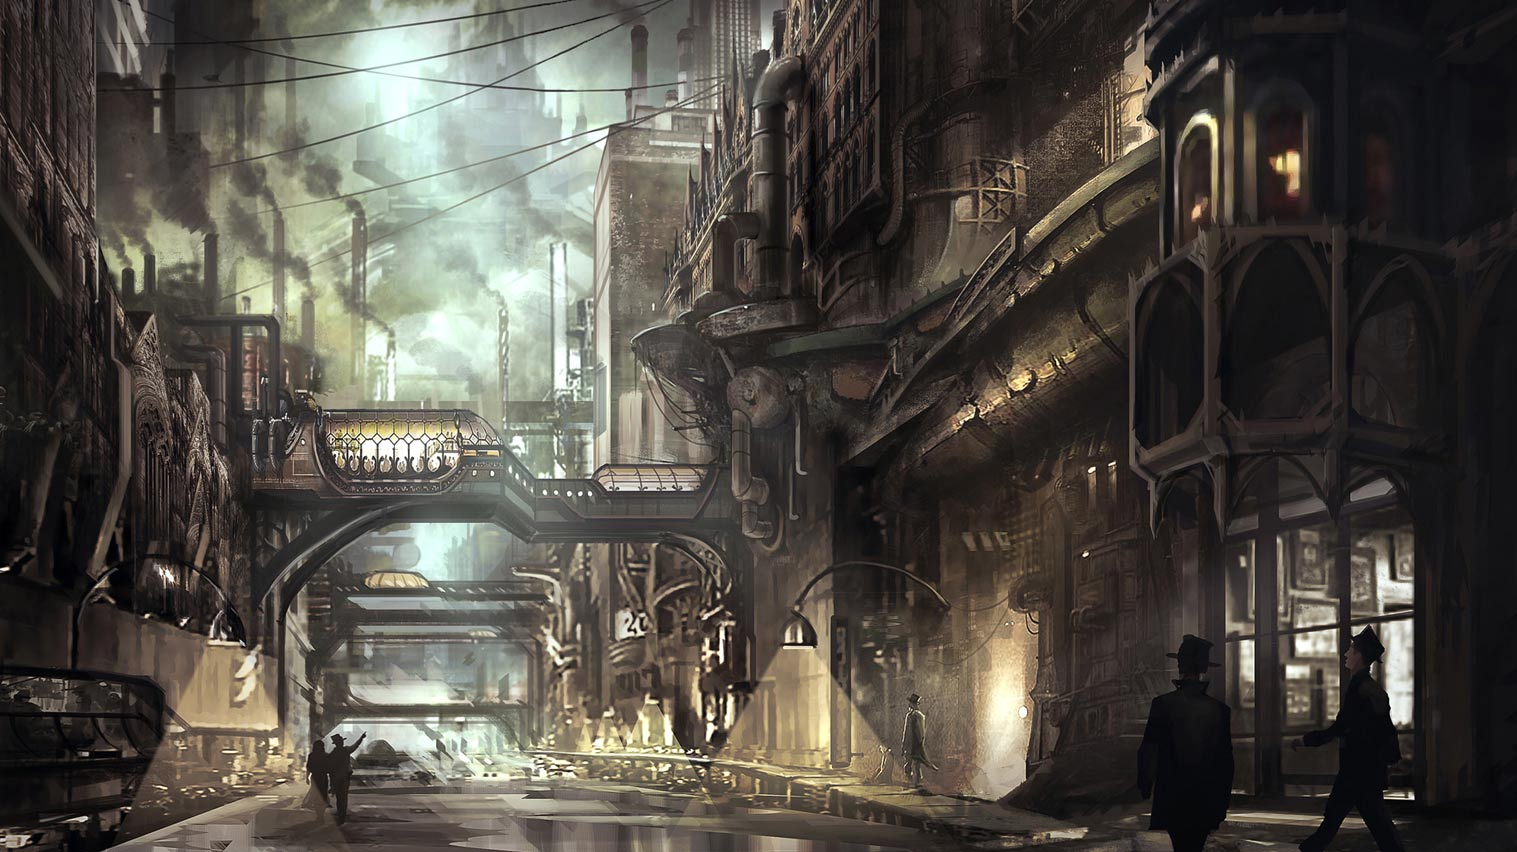
\includegraphics[width=\linewidth]{./images./Annexes/slide-04.jpg}
\\[-1mm]
\url{http://pocketguys.com}
\end{minipage}

\begin{minipage}{\textwidth}
	\begin{minipage}[c]{.49\textwidth}
	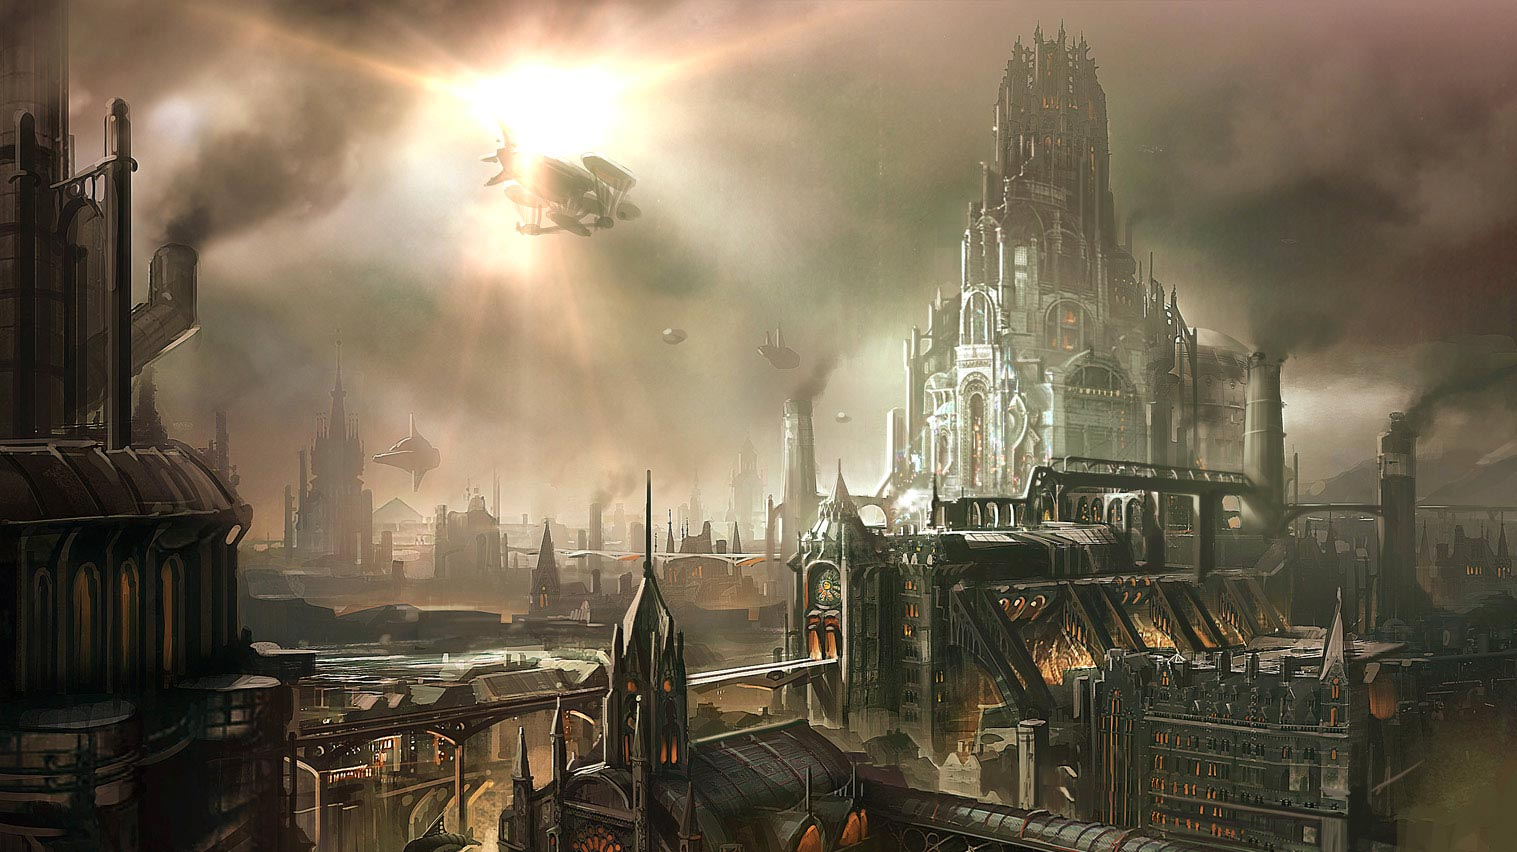
\includegraphics[width=\linewidth, height=4.9cm]{./images./Annexes/slide-02.jpg}
	\\[-1mm]\citeurl{TheScavengers_}
	
	\vspace{2mm}
	
	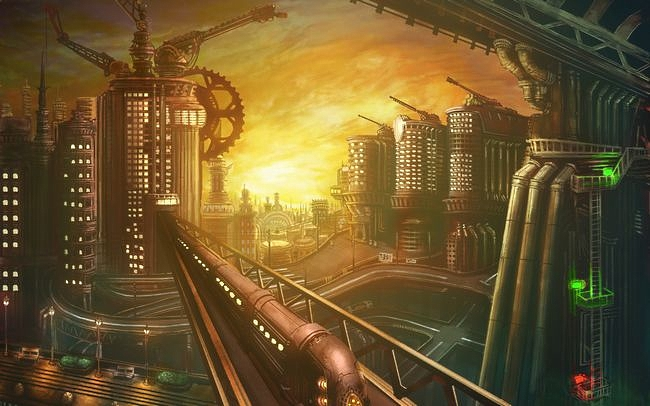
\includegraphics[width=\linewidth, height= 4.9cm]{./images./Annexes/sshot50fd39fccf53c.jpg}
	\\[-1mm]\citeurl{LateAfternoonTrainTravellingThroughaSteampunkCity_}
	\end{minipage}
	\hspace{.02\textwidth}
	\begin{minipage}[c]{.49\textwidth}
	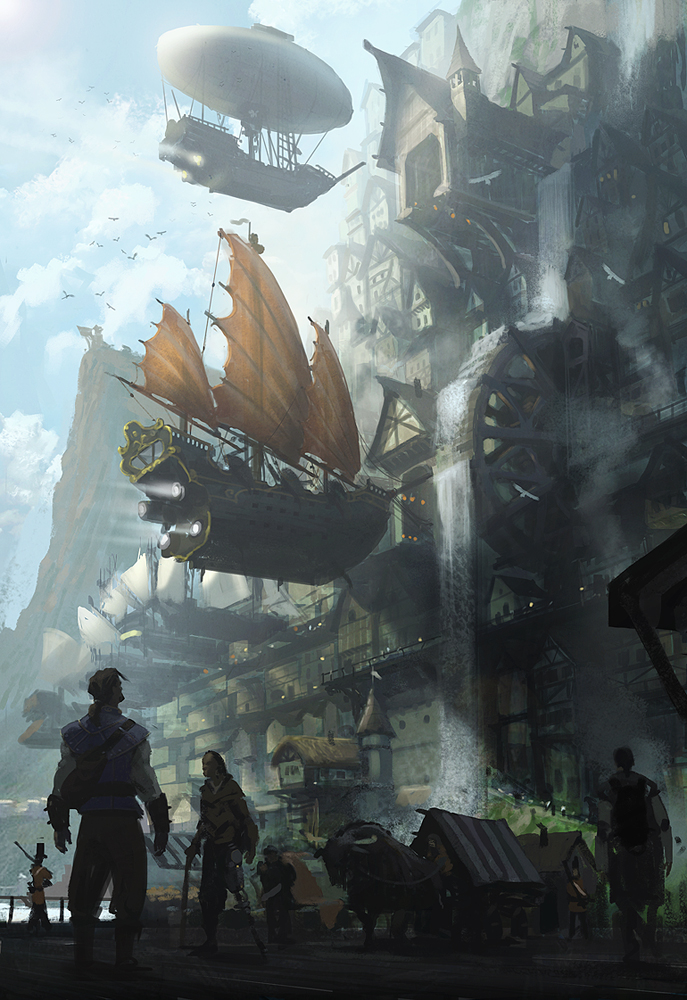
\includegraphics[width=\linewidth]{./images./Annexes/tumblr_mdbq3rCn4e1r4zno6o1_1280.jpg}
	\\[-1mm]\citeurl{SteampunkCityonPinterestSteampunkAirshipSteampunkIllustrationandLadyMechanika_}
	\end{minipage}

\end{minipage}






\titleformat{name=\chapter, numberless}[display]
{}
{}
{0pt}
{
	\fontsize{2cm}{1em}\selectfont\chapterfont
}

\printbibliography[notkeyword=image]

\printbibliography[keyword=image, title={Iconographie}]

%\printindex
%\newpage

\listoffigures

\listoftables

\begingroup
\let\clearpage\relax
\lstlistoflistings
\endgroup
\end{document}


